\documentclass{templateNote}
\usepackage{soul}
\begin{document}

\imagenlogoU{img/LogoElNube.png}
\linklogoU{https://github.com/MarceloPazPezo}
\linkQRDoc{https://github.com/MarceloPazPezo/MyRepo/blob/main/Icinf/Semestre\%207/Administraci\%C3\%B3n\%20y\%20Programaci\%C3\%B3n\%20de\%20Base\%20de\%20Datos/Guia\%20de\%20ejercicios\%20(Guia\%201)/Guia-1.pdf}
\titulo{Guía de ejercicios (Guía 1)}
\asignatura{Administración y Programación de Base de Datos}
\autor{
Marcelo Paz
}
\vDoc{1.2.0}

% Metadatos del PDF
\title{[\asignatura]-\titulo}
\author{
    \autor
}
\portada
\margenes % Crear márgenes
\section{Guía 1}
\begin{itemize}
    \item \textbf{Pregunta 1:} Utilizando RAID 6, para múltiples fallas de disco. Si fallan los siguientes discos, recuperar para dejar estable nuevamente.
    
    \begin{minipage}{0.5\textwidth}
        \begin{center}
            \begin{tabular}{|c|}
                \hline
                \textbf{D1) 11110000} \\
                \hline
                \textbf{D2) 10101010} \\
                \hline
                \textbf{D3) 00111000} \\
                \hline
                \textbf{D4) 01000001} \\
                \hline
            \end{tabular}
        \end{center}
    \end{minipage}
    \hfill
    \begin{minipage}{0.5\textwidth}
        \begin{tabular}{|c|c|c|c|c|c|c|}
            \hline
            1 & 2 & 3 & 4 & 5 & 6 & 7 \\ \hline
            1 & 1 & 1 & 0 & 1 & 0 & 0 \\
            1 & 1 & 0 & 1 & 0 & 1 & 0 \\
            1 & 0 & 1 & 1 & 0 & 0 & 1 \\ \hline
        \end{tabular}
    \end{minipage}
    Si fallan discos:
    \begin{itemize}
        \item 3 y 7.
        \textcolor{red}{
            \begin{align*}
                D3 &= D5 + D1 + D2 \\
                D7 &= D1 + D3 + D4
            \end{align*}
            Es necesario el D5:
            \begin{equation*}
                \begin{array}{ccccccccc}
                    & 1 & 1 & 1 & 1 & 0 & 0 & 0 & 0 \\
                    & 1 & 0 & 1 & 0 & 1 & 0 & 1 & 0 \\
                    & 0 & 0 & 1 & 1 & 1 & 0 & 0 & 0 \\ \hline
                D5: & 0 & 1 & 1 & 0 & 0 & 0 & 1 & 0 \\
                \end{array}
            \end{equation*}
            Luego se calcula D3:
            \begin{equation*}
                \begin{array}{ccccccccc}
                    & 0 & 1 & 1 & 0 & 0 & 0 & 1 & 0 \\
                    & 1 & 1 & 1 & 1 & 0 & 0 & 0 & 0 \\
                    & 1 & 0 & 1 & 0 & 1 & 0 & 1 & 0 \\ \hline
                D3: & 0 & 0 & 1 & 1 & 1 & 0 & 0 & 0 \\
                \end{array}
            \end{equation*}
            Finalmente se calcula D7:
            \begin{equation*}
                \begin{array}{ccccccccc}
                    & 1 & 1 & 1 & 1 & 0 & 0 & 0 & 0 \\
                    & 0 & 0 & 1 & 1 & 1 & 0 & 0 & 0 \\
                    & 0 & 1 & 0 & 0 & 0 & 0 & 0 & 1 \\ \hline
                D7: & 1 & 0 & 0 & 0 & 1 & 0 & 0 & 1 \\
                \end{array}
            \end{equation*}
        }
        \item 1 y 6.
        \textcolor{red}{
            \begin{align*}
                D1 &= D5 + D2 + D3 \\
                D6 &= D1 + D2 + D4
            \end{align*}
            Es necesario el D5:
            \begin{equation*}
                \begin{array}{ccccccccc}
                    & 1 & 1 & 1 & 1 & 0 & 0 & 0 & 0 \\
                    & 1 & 0 & 1 & 0 & 1 & 0 & 1 & 0 \\
                    & 0 & 0 & 1 & 1 & 1 & 0 & 0 & 0 \\ \hline
                D5: & 0 & 1 & 1 & 0 & 0 & 0 & 1 & 0 \\
                \end{array}
            \end{equation*}
            Luego se calcula D1:
            \begin{equation*}
                \begin{array}{ccccccccc}
                    & 0 & 1 & 1 & 0 & 0 & 0 & 1 & 0 \\
                    & 1 & 0 & 1 & 0 & 1 & 0 & 1 & 0 \\
                    & 0 & 0 & 1 & 1 & 1 & 0 & 0 & 0 \\ \hline
                D1: & 1 & 1 & 1 & 1 & 0 & 0 & 0 & 0 \\
                \end{array}
            \end{equation*}
            Finalmente se calcula D6:
            \begin{equation*}
                \begin{array}{ccccccccc}
                    & 1 & 1 & 1 & 1 & 0 & 0 & 0 & 0 \\
                    & 1 & 0 & 1 & 0 & 1 & 0 & 1 & 0 \\
                    & 0 & 1 & 0 & 0 & 0 & 0 & 0 & 1 \\ \hline
                D6: & 0 & 0 & 0 & 1 & 1 & 0 & 1 & 1 \\
                \end{array}
            \end{equation*}
        }
        \item 2 y 6.
        \textcolor{red}{
            \begin{align*}
                D2 &= D5 + D1 + D3 \\
                D6 &= D1 + D2 + D4
            \end{align*}
            Es necesario el D5:
            \begin{equation*}
                \begin{array}{ccccccccc}
                    & 1 & 1 & 1 & 1 & 0 & 0 & 0 & 0 \\
                    & 1 & 0 & 1 & 0 & 1 & 0 & 1 & 0 \\
                    & 0 & 0 & 1 & 1 & 1 & 0 & 0 & 0 \\ \hline
                D5: & 0 & 1 & 1 & 0 & 0 & 0 & 1 & 0 \\
                \end{array}
            \end{equation*}
            Luego se calcula D2:
            \begin{equation*}
                \begin{array}{ccccccccc}
                    & 0 & 1 & 1 & 0 & 0 & 0 & 1 & 0 \\
                    & 1 & 1 & 1 & 1 & 0 & 0 & 0 & 0 \\
                    & 0 & 0 & 1 & 1 & 1 & 0 & 0 & 0 \\ \hline
                D2: & 1 & 0 & 1 & 0 & 1 & 0 & 1 & 0 \\
                \end{array}
            \end{equation*}
            Finalmente se calcula D6:
            \begin{equation*}
                \begin{array}{ccccccccc}
                    & 1 & 1 & 1 & 1 & 0 & 0 & 0 & 0 \\
                    & 1 & 0 & 1 & 0 & 1 & 0 & 1 & 0 \\
                    & 0 & 1 & 0 & 0 & 0 & 0 & 0 & 1 \\ \hline
                D6: & 0 & 0 & 0 & 1 & 1 & 0 & 1 & 1 \\
                \end{array}
            \end{equation*}
        }
        \item 3 y 5.
        \textcolor{red}{
            \begin{align*}
                D3 &= D7 + D1 + D4 \\
                D5 &= D1 + D2 + D3
            \end{align*}
            Es necesario el D7:
            \begin{equation*}
                \begin{array}{ccccccccc}
                    & 1 & 1 & 1 & 1 & 0 & 0 & 0 & 0 \\
                    & 0 & 0 & 1 & 1 & 1 & 0 & 0 & 0 \\
                    & 0 & 1 & 0 & 0 & 0 & 0 & 0 & 1 \\ \hline
                D7: & 1 & 0 & 0 & 0 & 1 & 0 & 0 & 1 \\
                \end{array}
            \end{equation*}
            Luego se calcula D3:
            \begin{equation*}
                \begin{array}{ccccccccc}
                    & 0 & 1 & 1 & 0 & 0 & 0 & 1 & 0 \\
                    & 1 & 1 & 1 & 1 & 0 & 0 & 0 & 0 \\
                    & 0 & 0 & 1 & 1 & 1 & 0 & 0 & 0 \\ \hline
                D3: & 1 & 0 & 1 & 0 & 1 & 0 & 1 & 0 \\
                \end{array}
            \end{equation*}
            Finalmente se calcula D5:
            \begin{equation*}
                \begin{array}{ccccccccc}
                    & 1 & 1 & 1 & 1 & 0 & 0 & 0 & 0 \\
                    & 1 & 0 & 1 & 0 & 1 & 0 & 1 & 0 \\
                    & 0 & 0 & 1 & 1 & 1 & 0 & 0 & 0 \\ \hline
                D5: & 0 & 1 & 1 & 0 & 0 & 0 & 1 & 0 \\
                \end{array}
            \end{equation*}
        }
        \item 4 y 7.
        \textcolor{red}{
            \begin{align*}
                D4 &= D6 + D1 + D2 \\
                D7 &= D1 + D3 + D4
            \end{align*}
            Es necesario el D6:
            \begin{equation*}
                \begin{array}{ccccccccc}
                    & 1 & 1 & 1 & 1 & 0 & 0 & 0 & 0 \\
                    & 1 & 0 & 1 & 0 & 1 & 0 & 1 & 0 \\
                    & 0 & 1 & 0 & 0 & 0 & 0 & 0 & 1 \\ \hline
                D6: & 0 & 0 & 0 & 1 & 1 & 0 & 1 & 1 \\
                \end{array}
            \end{equation*}
            Luego se calcula D4:
            \begin{equation*}
                \begin{array}{ccccccccc}
                    & 0 & 0 & 0 & 1 & 1 & 0 & 1 & 1 \\
                    & 1 & 1 & 1 & 1 & 0 & 0 & 0 & 0 \\
                    & 1 & 0 & 1 & 0 & 1 & 0 & 1 & 0 \\ \hline
                D4: & 0 & 1 & 0 & 0 & 0 & 0 & 0 & 1 \\
                \end{array}
            \end{equation*}
            Finalmente se calcula D7:
            \begin{equation*}
                \begin{array}{ccccccccc}
                    & 1 & 1 & 1 & 1 & 0 & 0 & 0 & 0 \\
                    & 0 & 0 & 1 & 1 & 1 & 0 & 0 & 0 \\
                    & 0 & 1 & 0 & 0 & 0 & 0 & 0 & 1 \\ \hline
                D7: & 1 & 0 & 0 & 0 & 1 & 0 & 0 & 1 \\
                \end{array}
            \end{equation*}
        }
    \end{itemize}

    \item \textbf{Pregunta 2:} Utilizando Hash extensible. Suponer que las llaves son Hash en secuencias de 4 bits. Los bloques pueden contener 3 registros. Si se comienza con una tabla hash con dos bloques vacíos (correspondientes a 0 y 1). Mostrar la organización después de insertar con llaves:
    
    \textbf{Hash inicial:}
    \begin{center}
        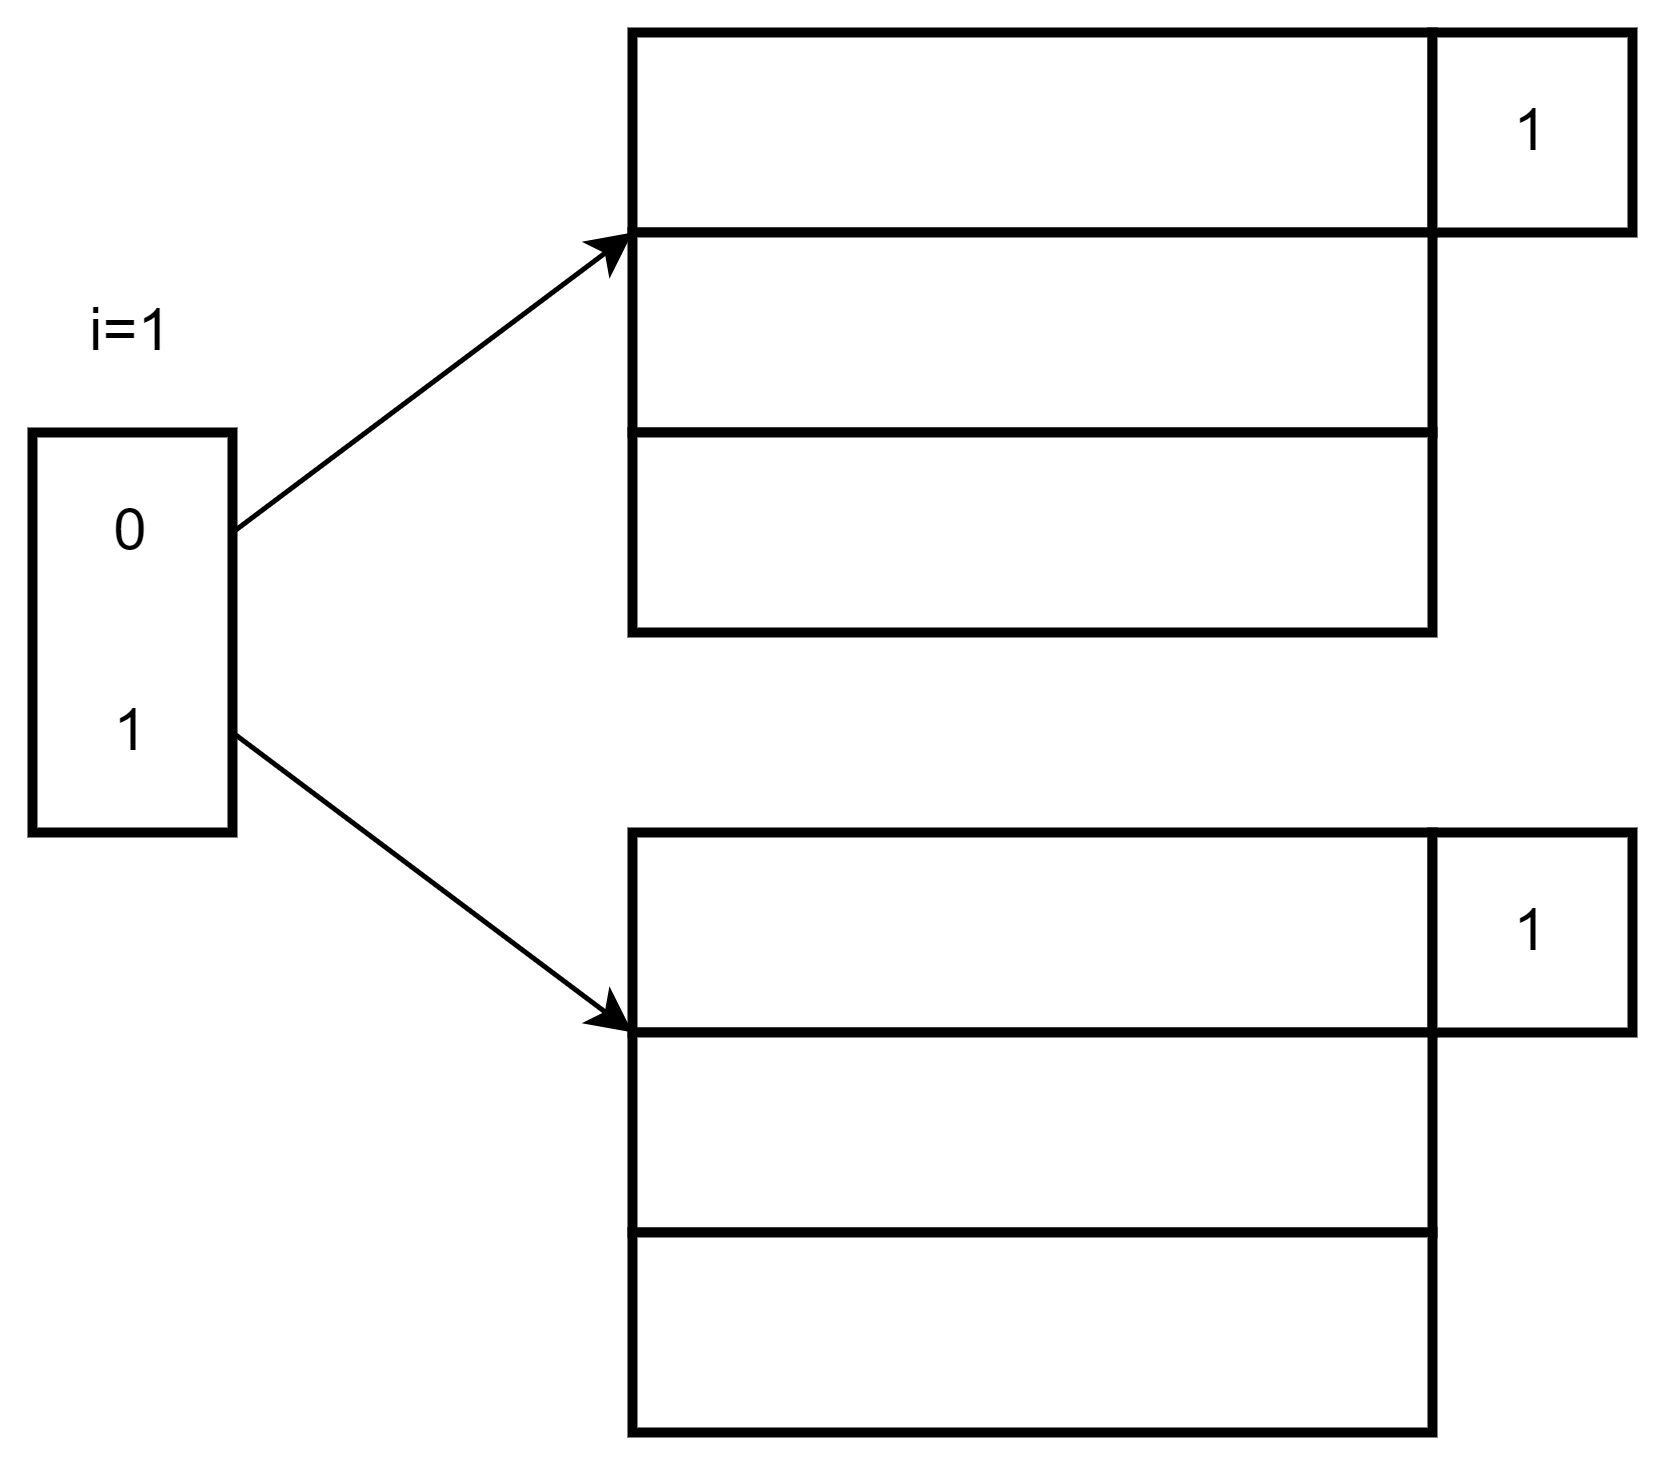
\includegraphics[width=0.4\textwidth]{diagram/Problema2.png}
    \end{center}
    \begin{enumerate}
        \item 1001, 0001, 1100, 1010, 0000, 0111, 1000.
        
        \textcolor{red}{
            Ingresamos 1001:
            \begin{center}
                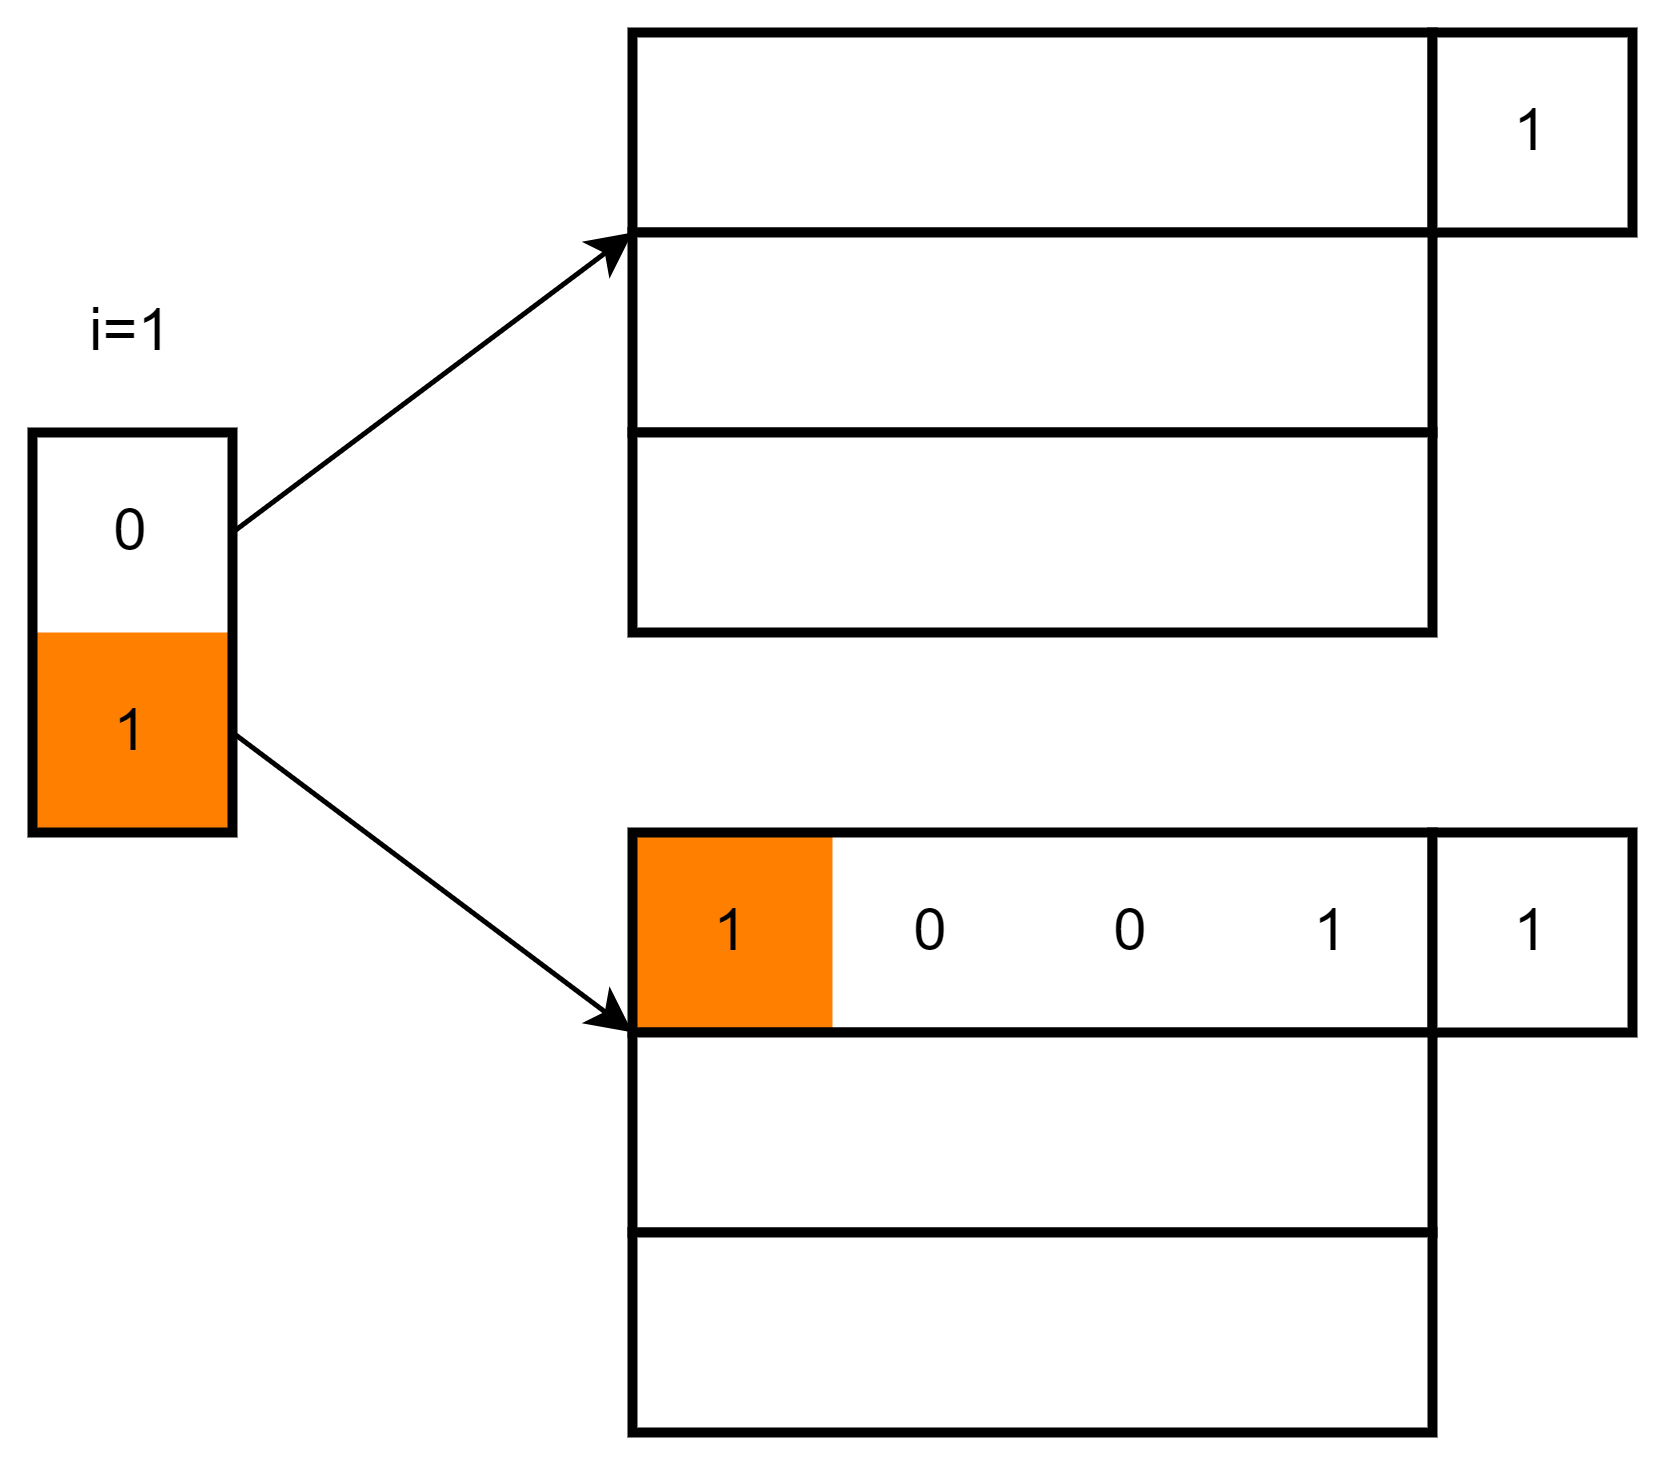
\includegraphics[width=0.4\textwidth]{diagram/Problema2-11.png}
            \end{center}
            Ingresamos 0001:
            \begin{center}
                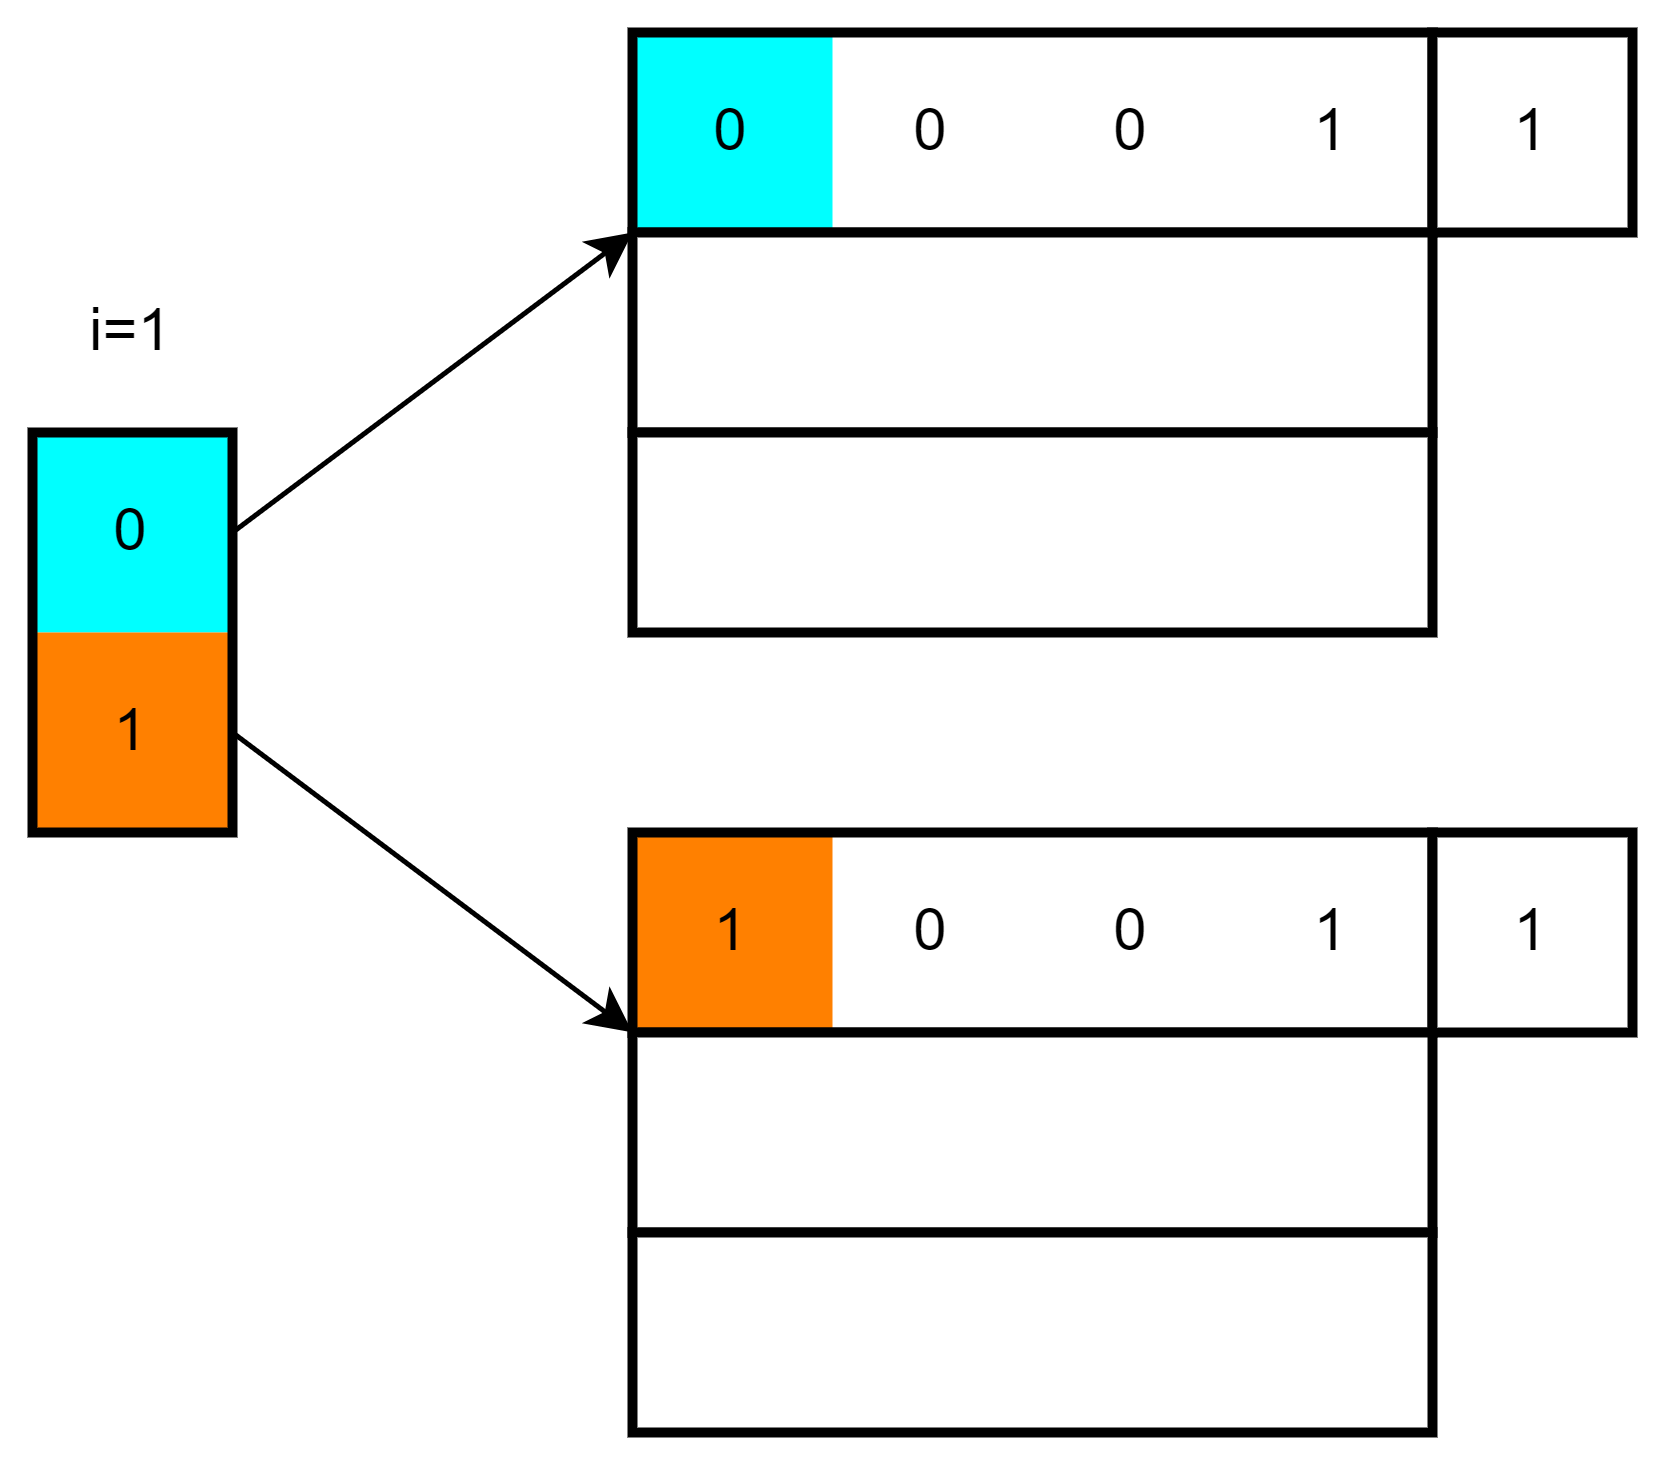
\includegraphics[width=0.4\textwidth]{diagram/Problema2-12.png}
            \end{center}
            \newpage
            Ingresamos 1100:
            \begin{center}
                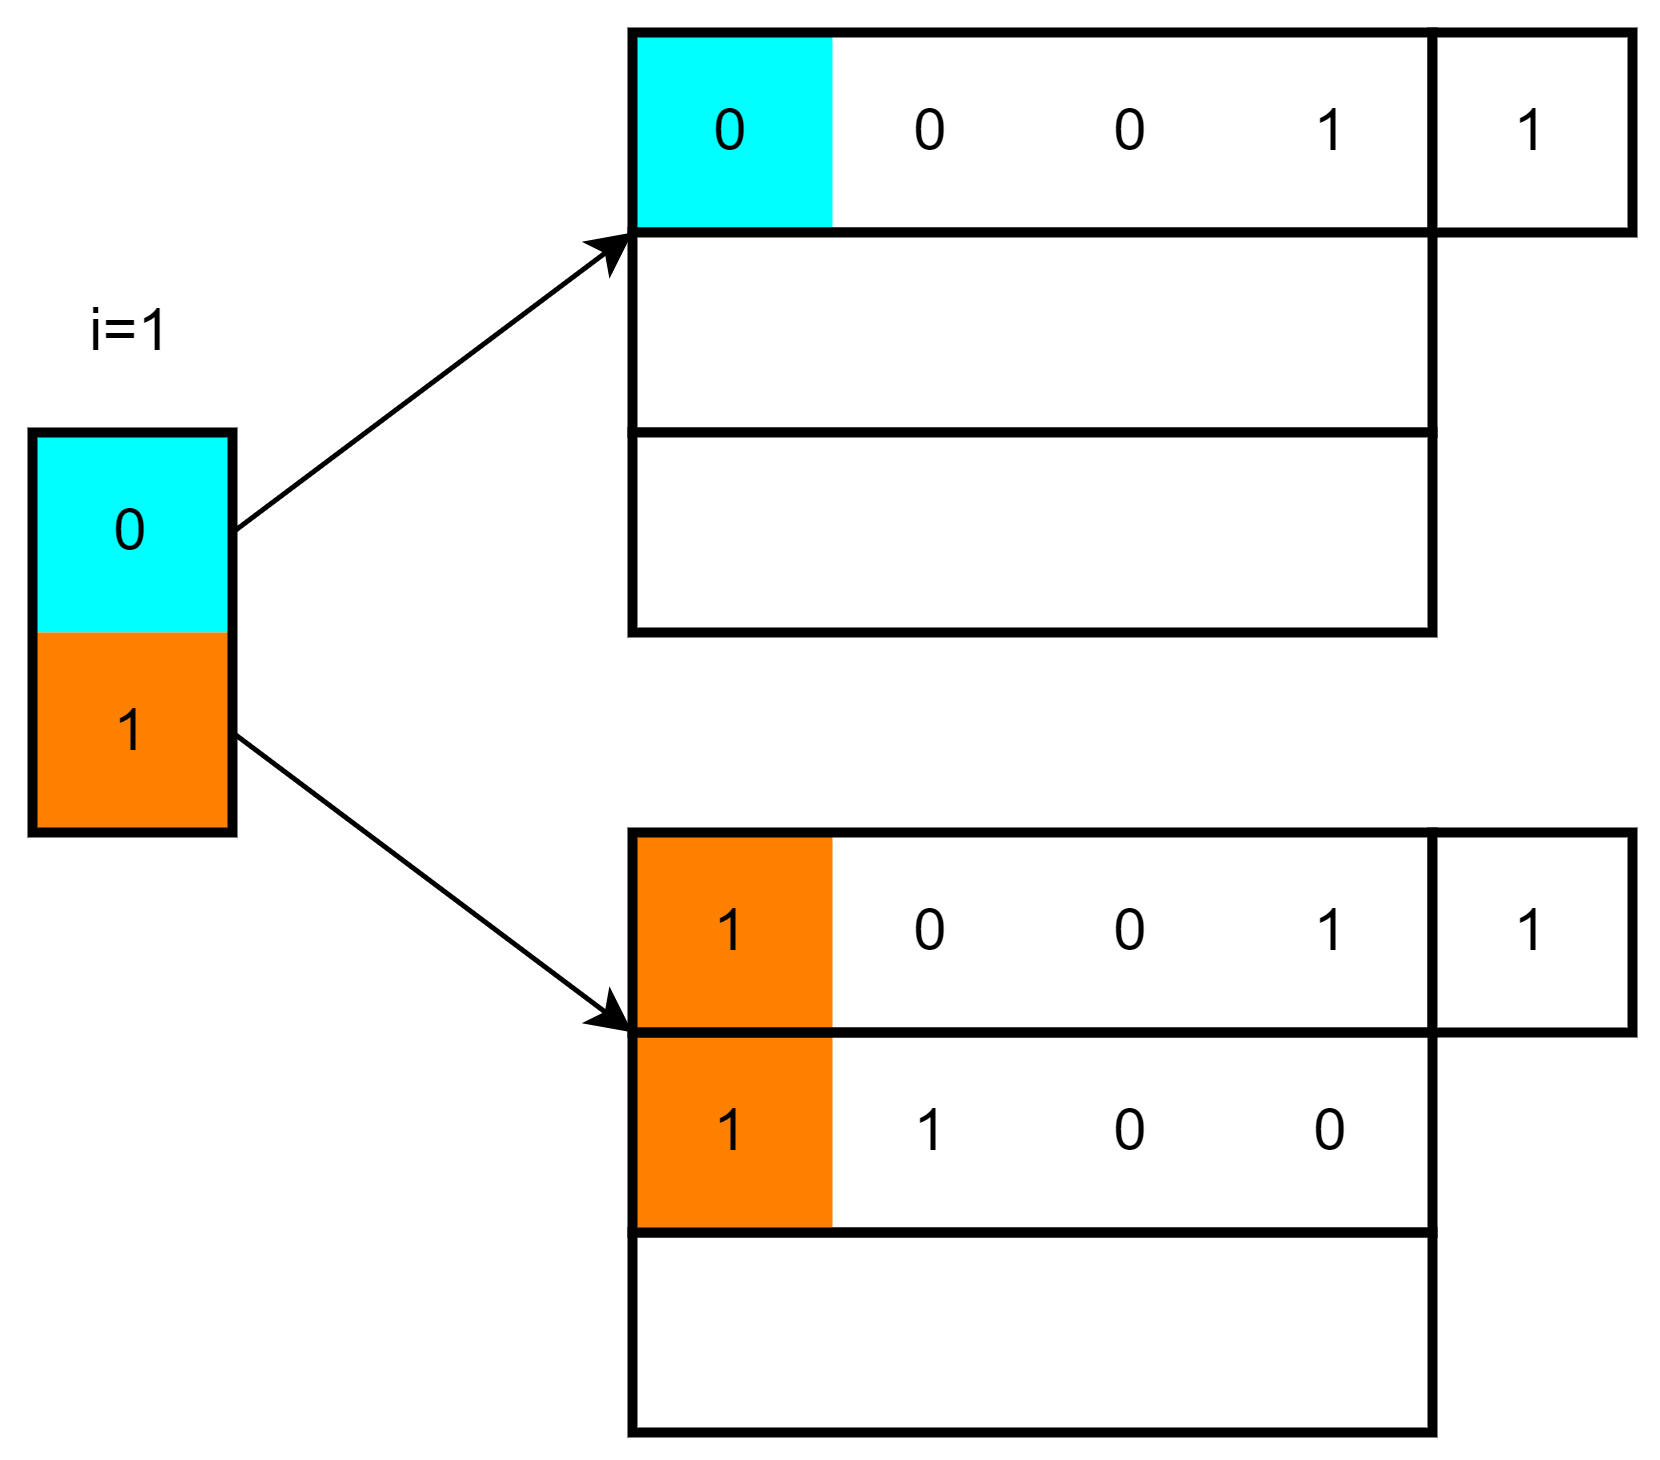
\includegraphics[width=0.4\textwidth]{diagram/Problema2-13.png}
            \end{center}
            Ingresamos 1010:
            \begin{center}
                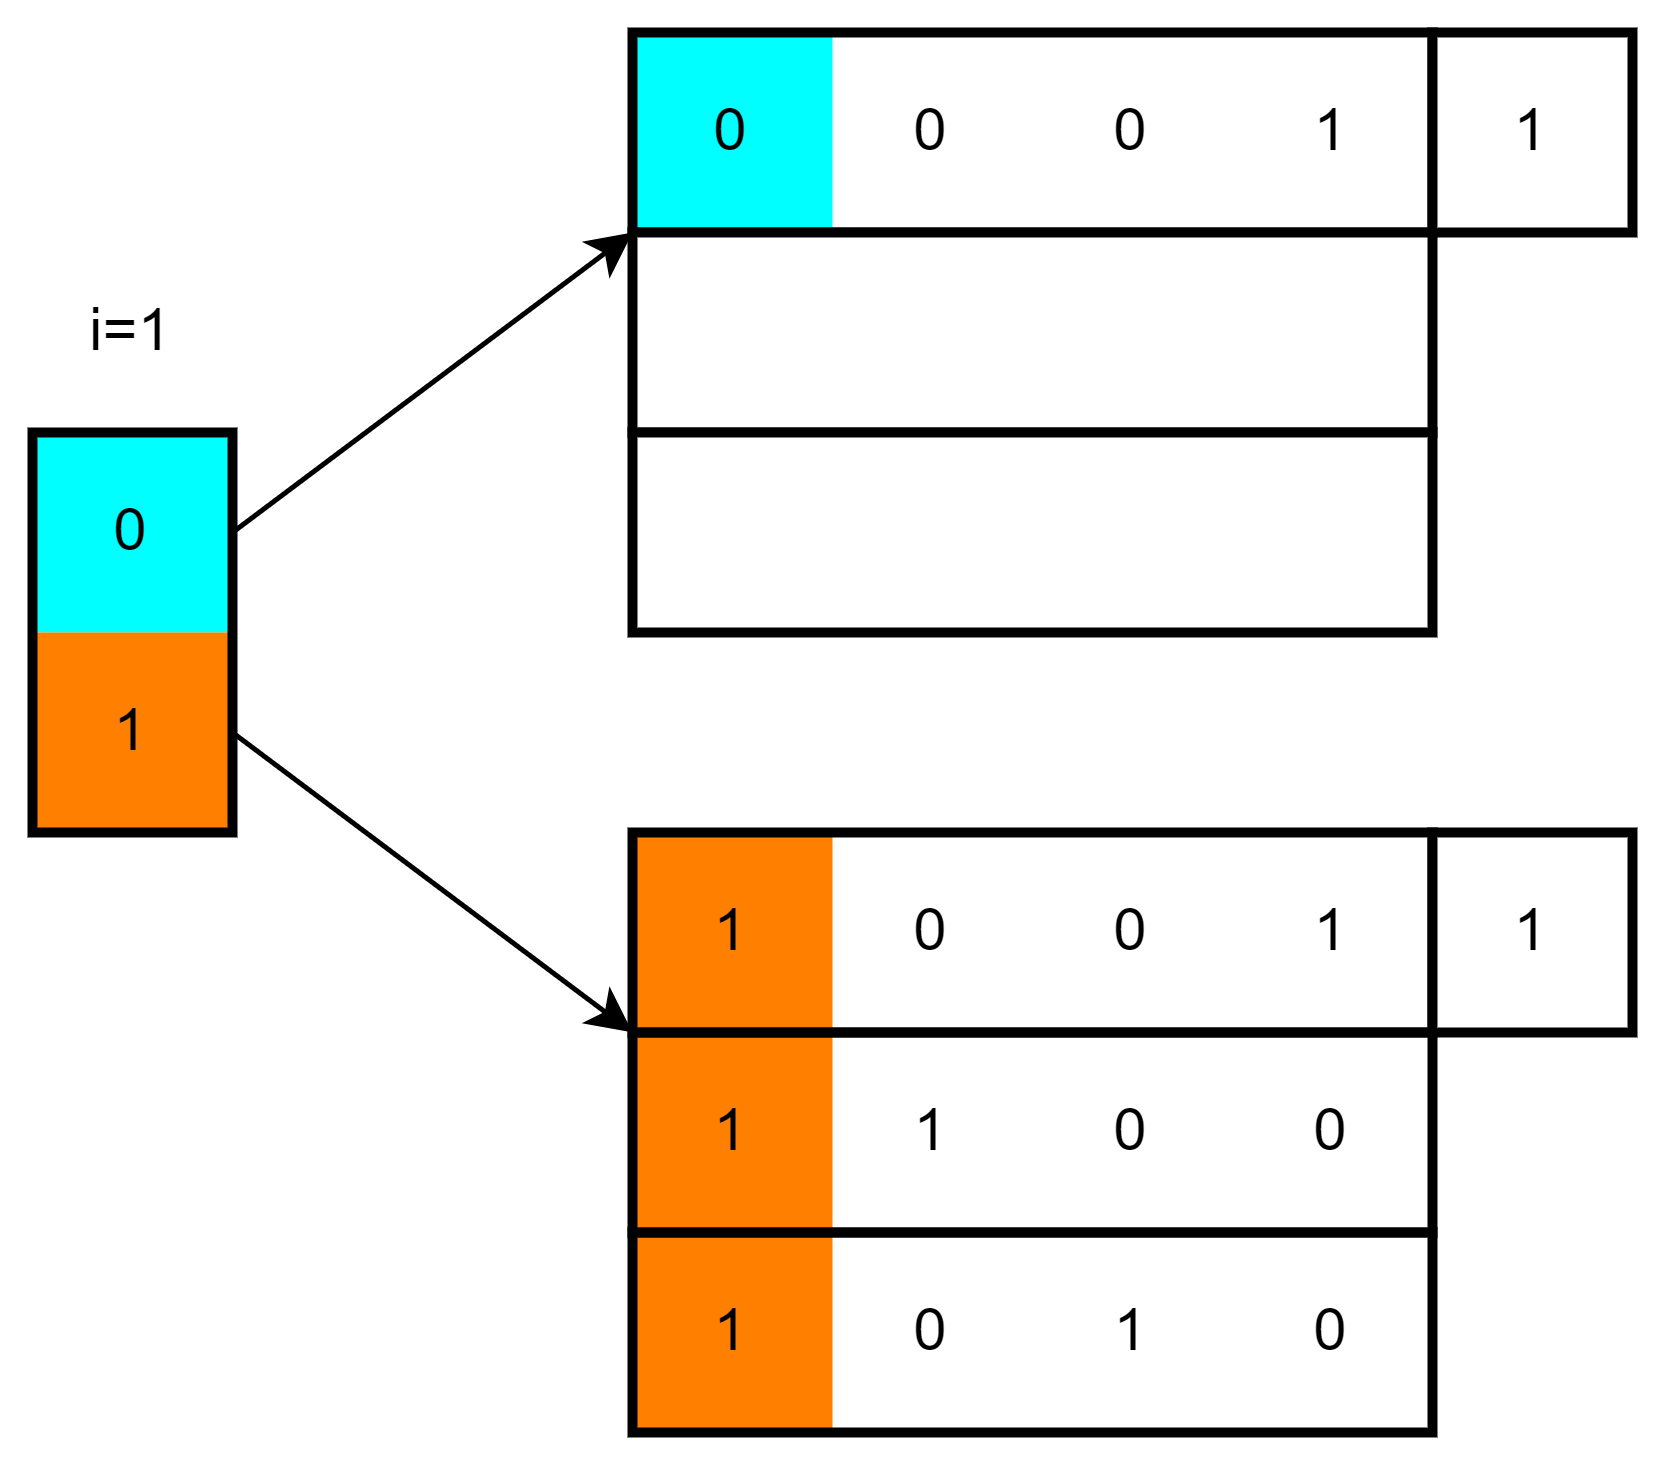
\includegraphics[width=0.4\textwidth]{diagram/Problema2-14.png}
            \end{center}
            Ingresamos 0000:
            \begin{center}
                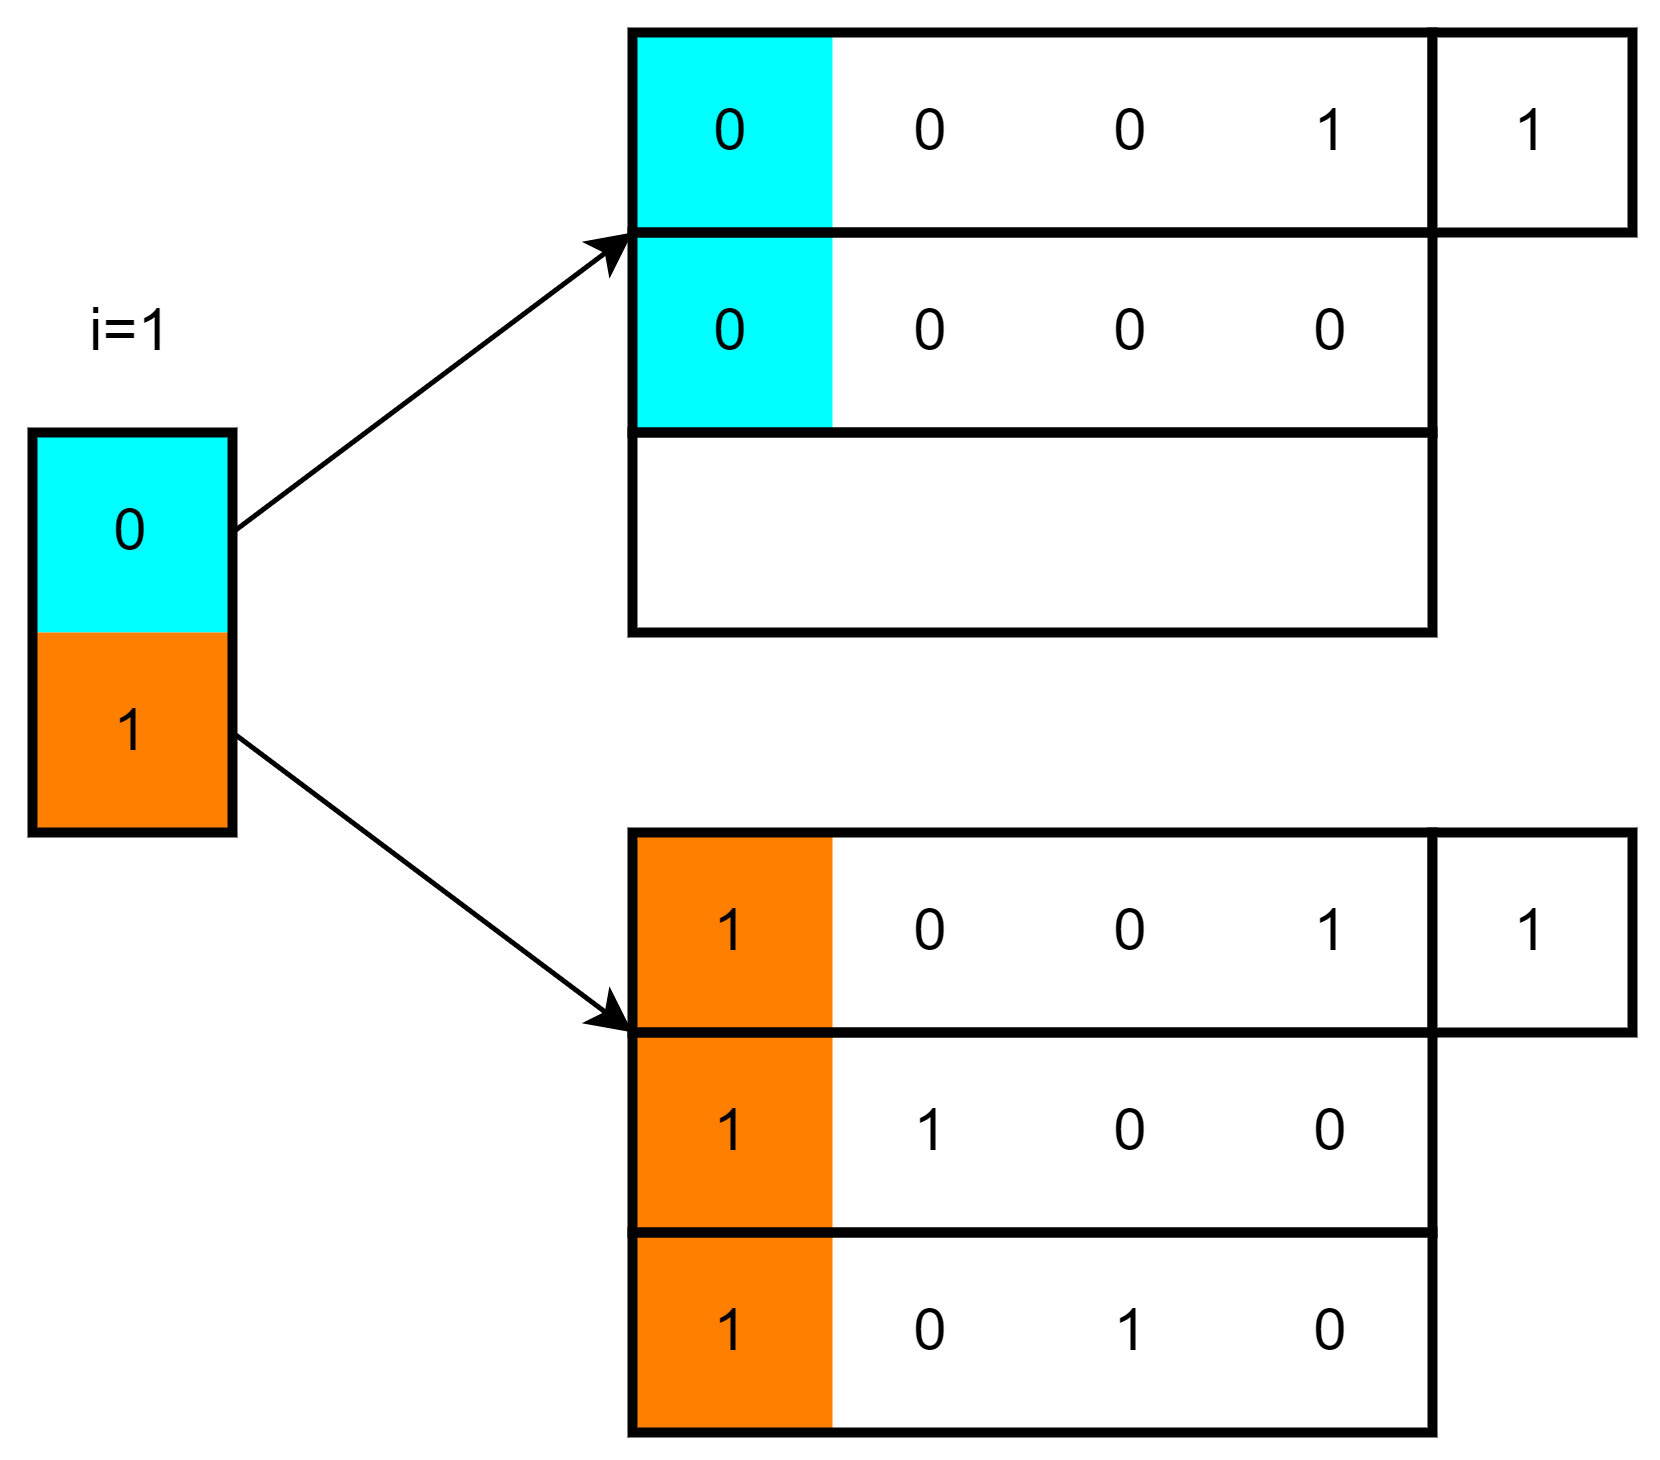
\includegraphics[width=0.4\textwidth]{diagram/Problema2-15.png}
            \end{center}
            \newpage
            Ingresamos 0111:
            \begin{center}
                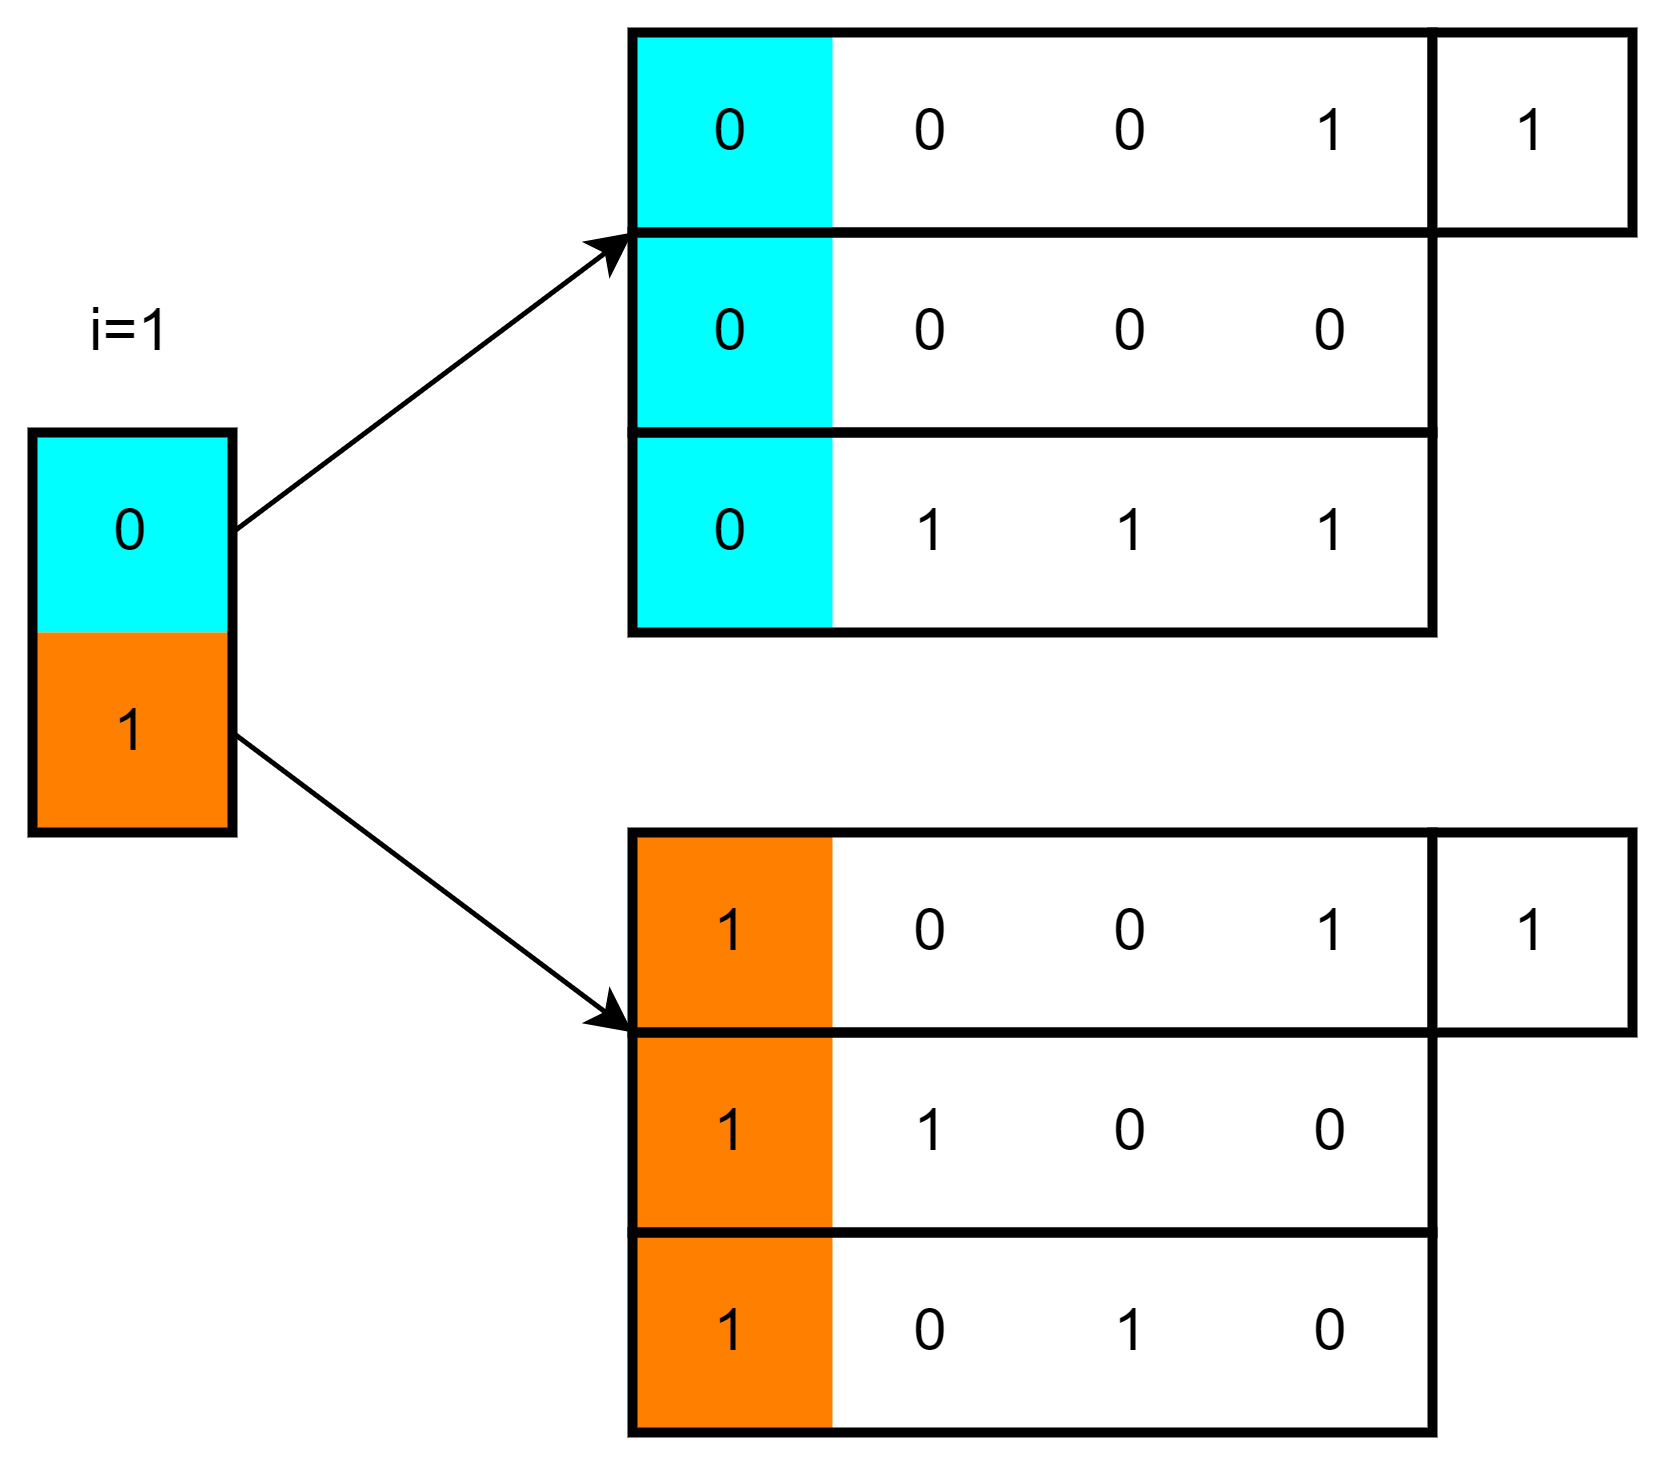
\includegraphics[width=0.4\textwidth]{diagram/Problema2-16.png}
            \end{center}
            Ingresamos 1000:
            \begin{center}
                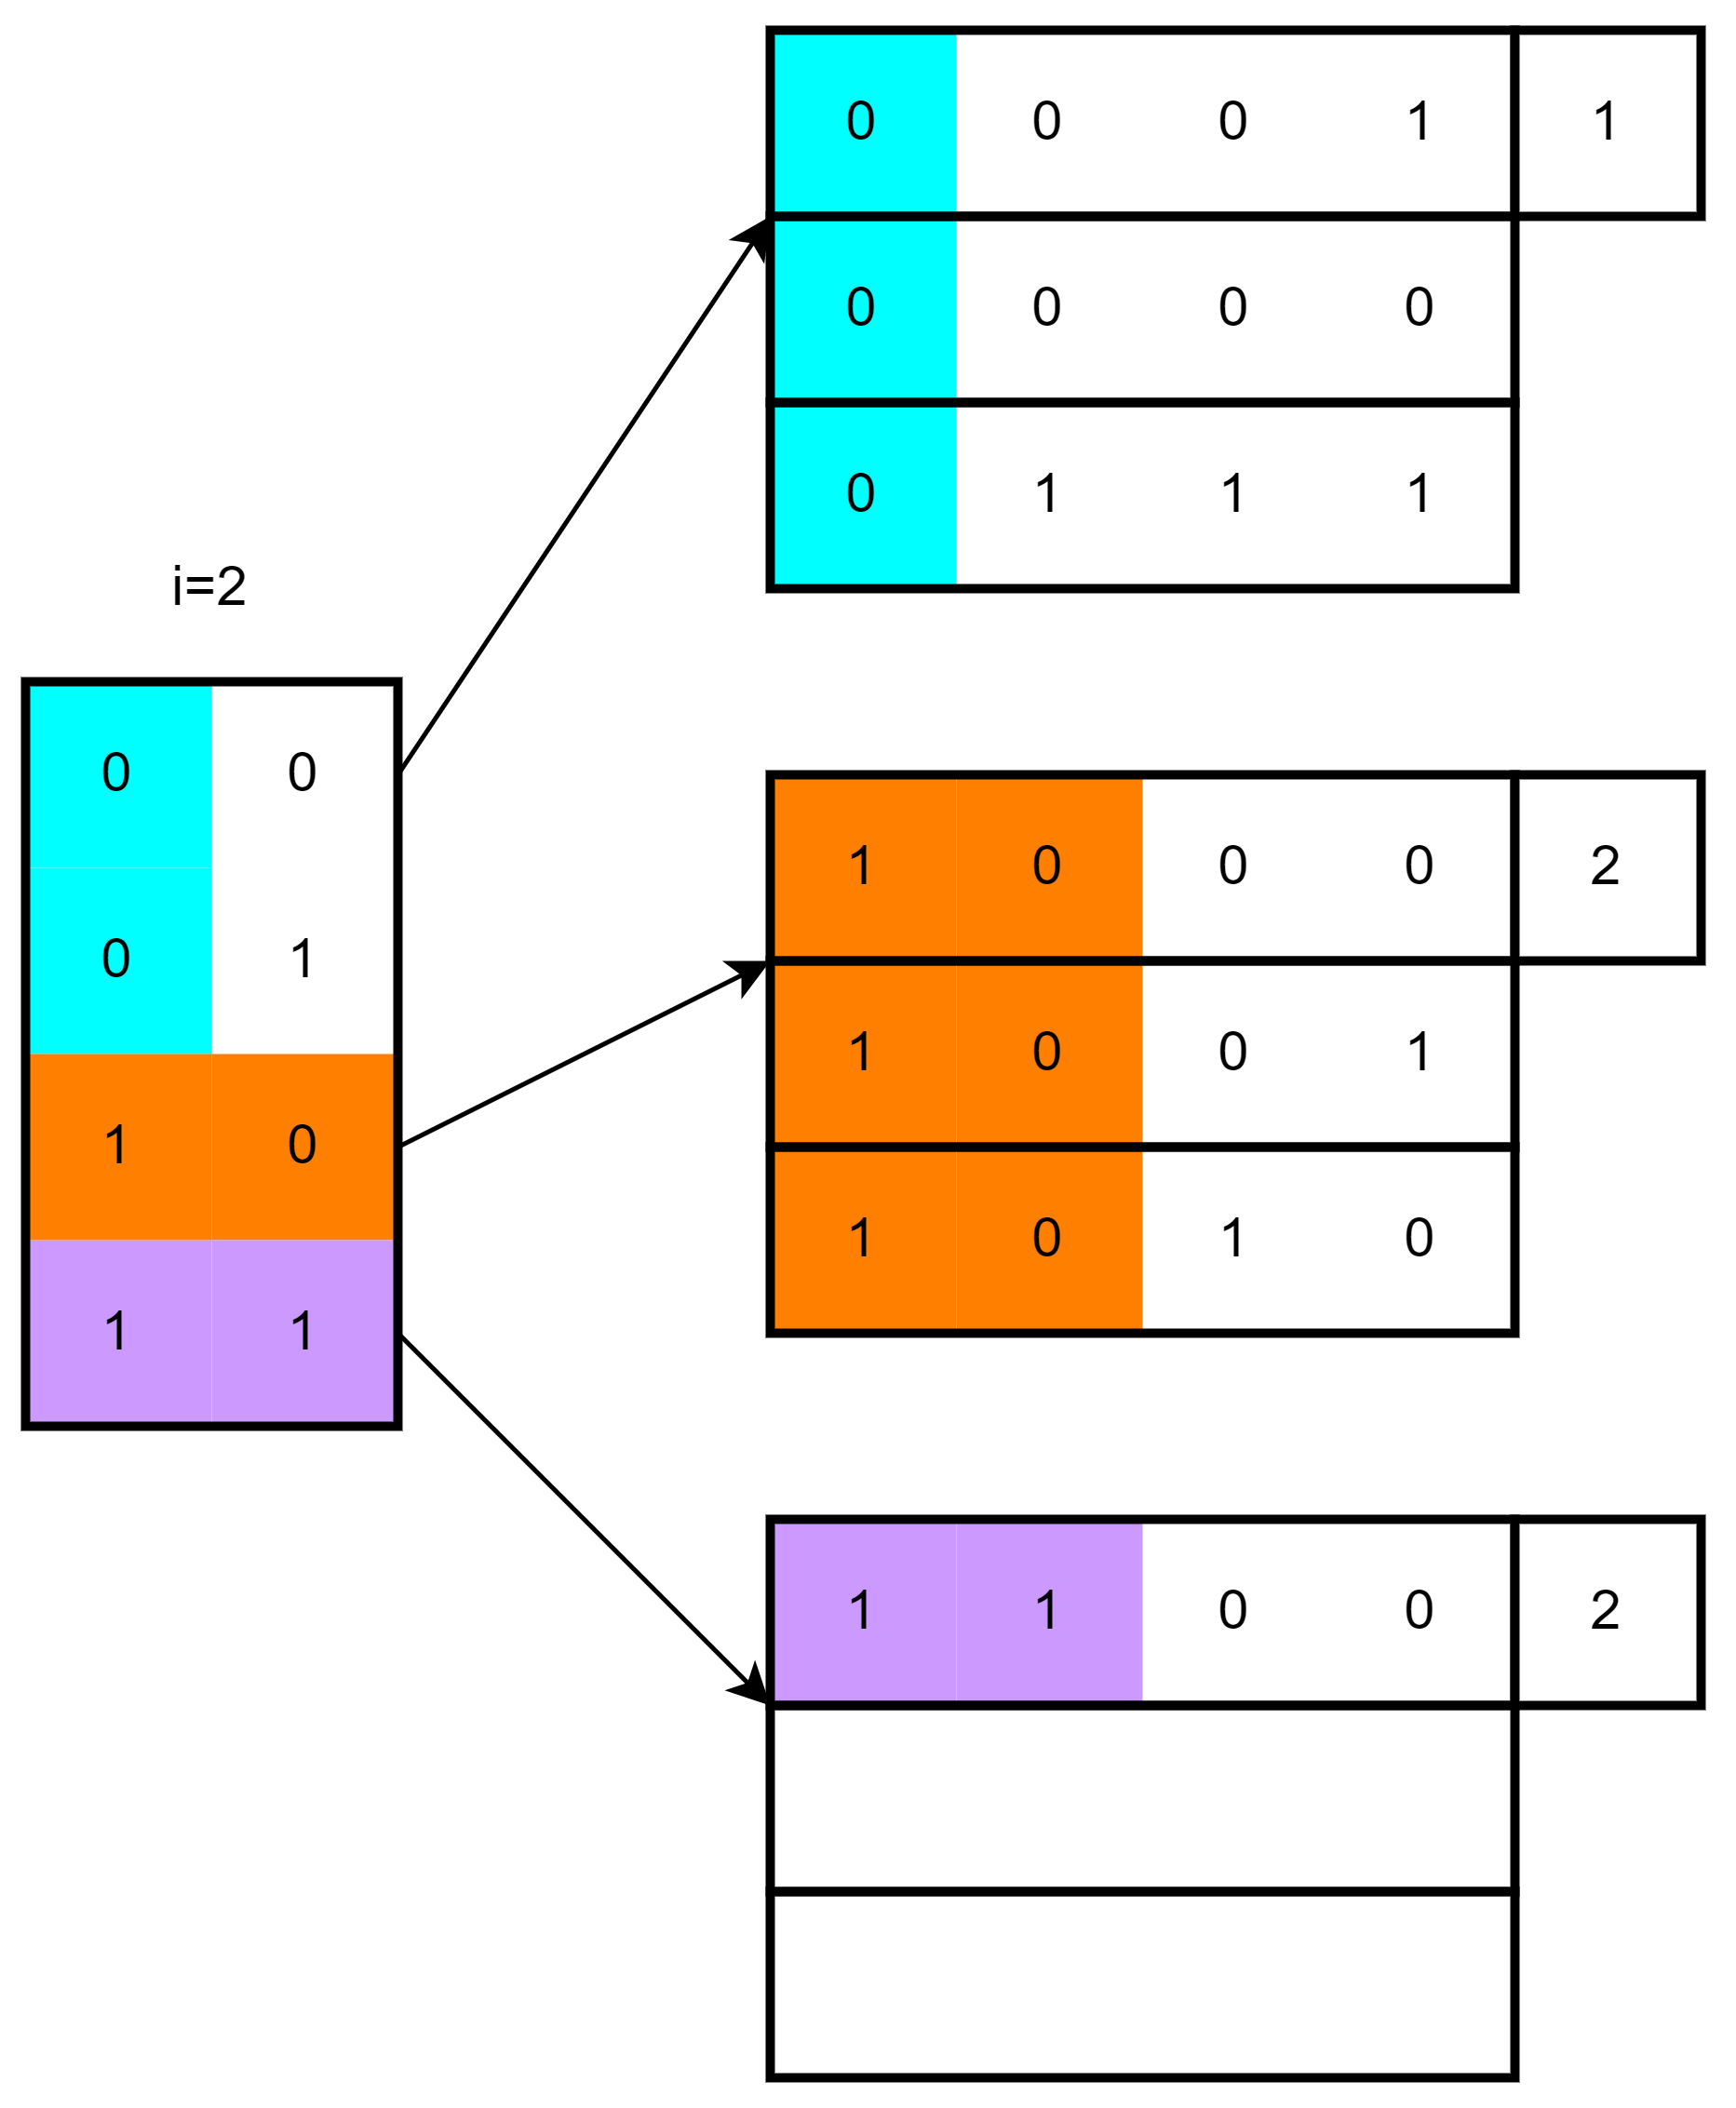
\includegraphics[width=0.4\textwidth]{diagram/Problema2-17.png}
            \end{center}
        }
        
        \newpage
        \item 1111, 1110, 1101, 1100.
        
        \textcolor{red}{
            Ingresamos 1111:
            \begin{center}
                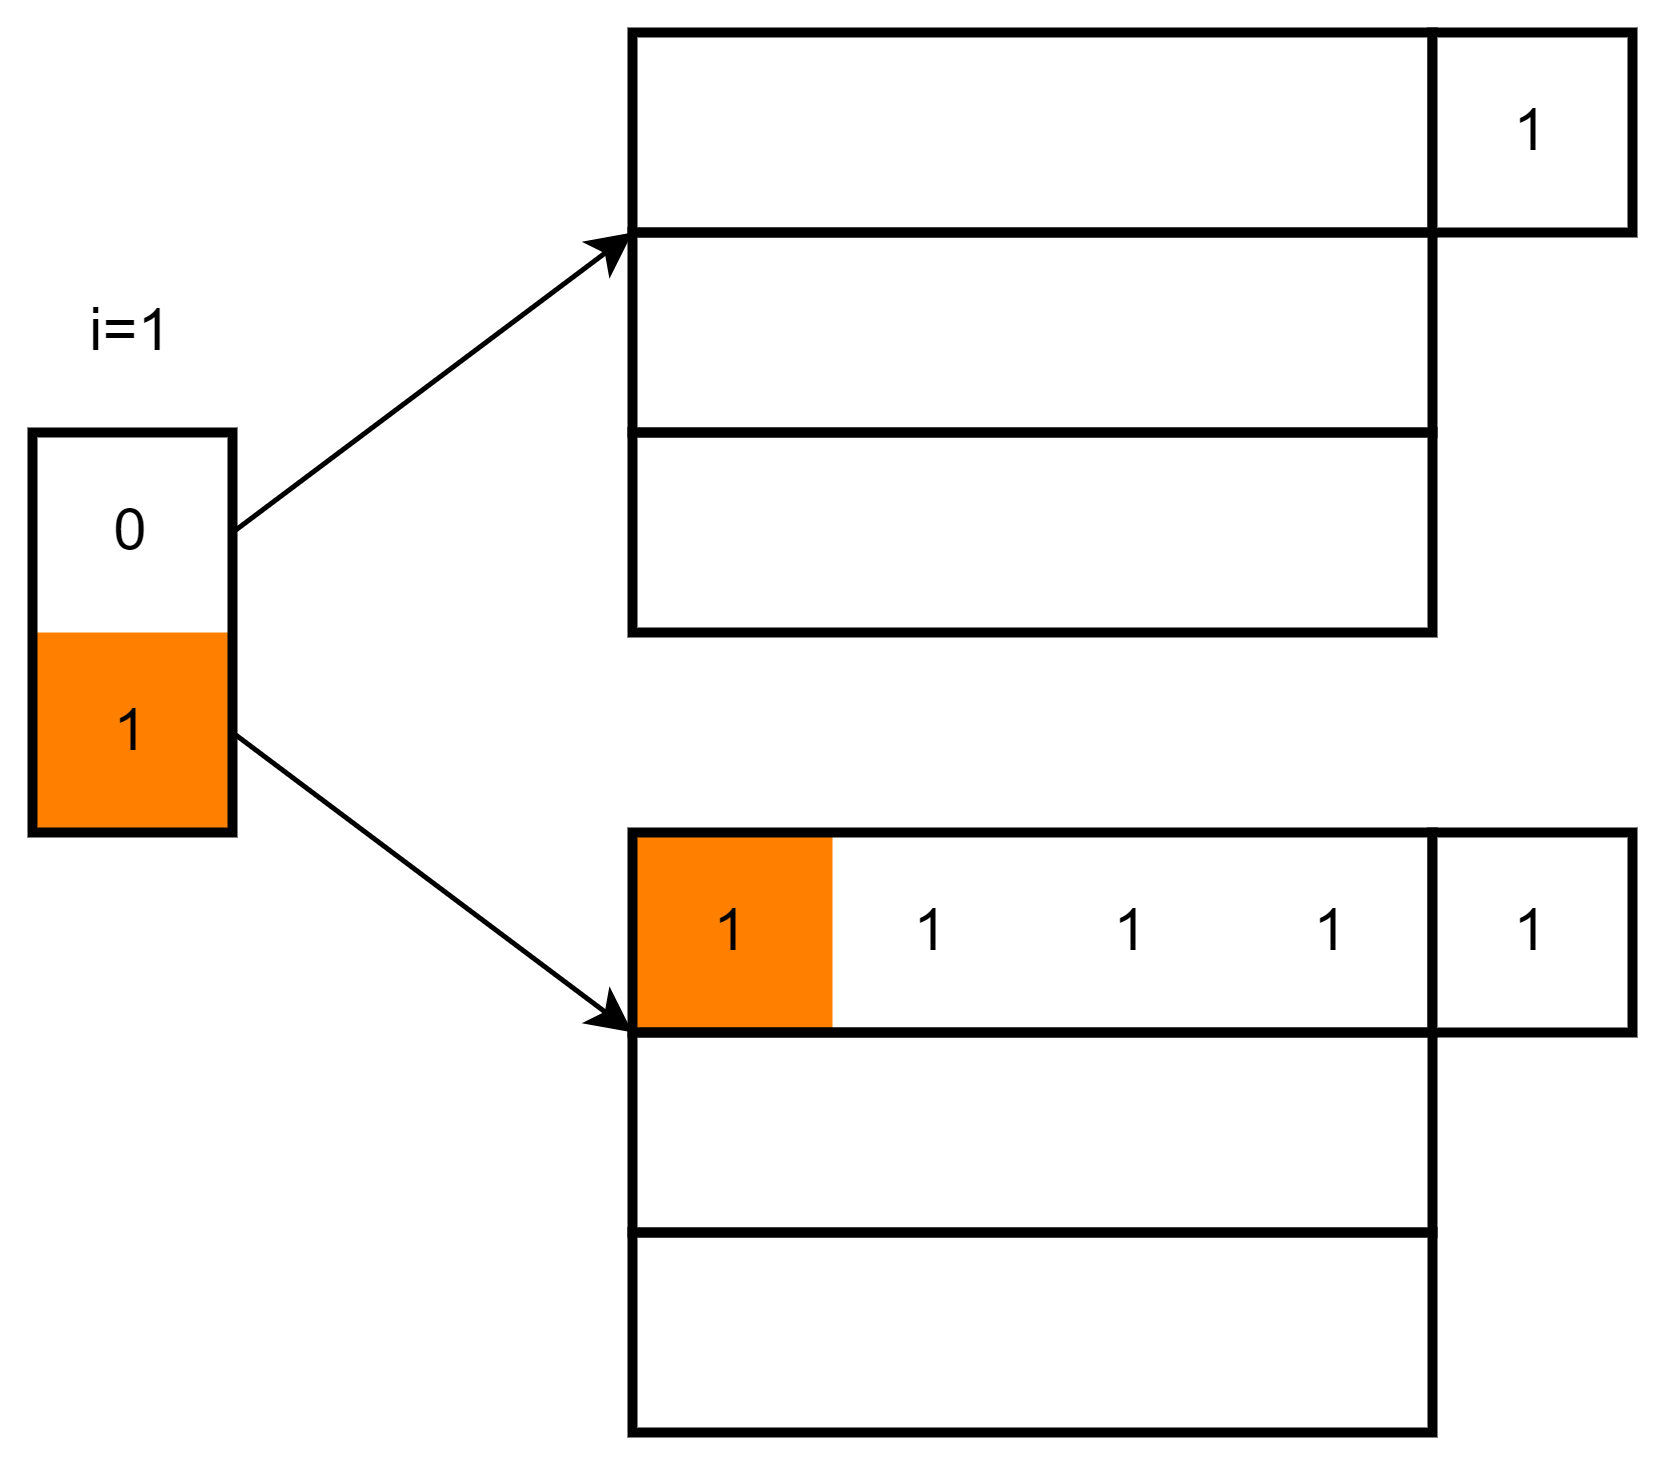
\includegraphics[width=0.4\textwidth]{diagram/Problema2-21.png}
            \end{center}
            Ingresamos 1110:
            \begin{center}
                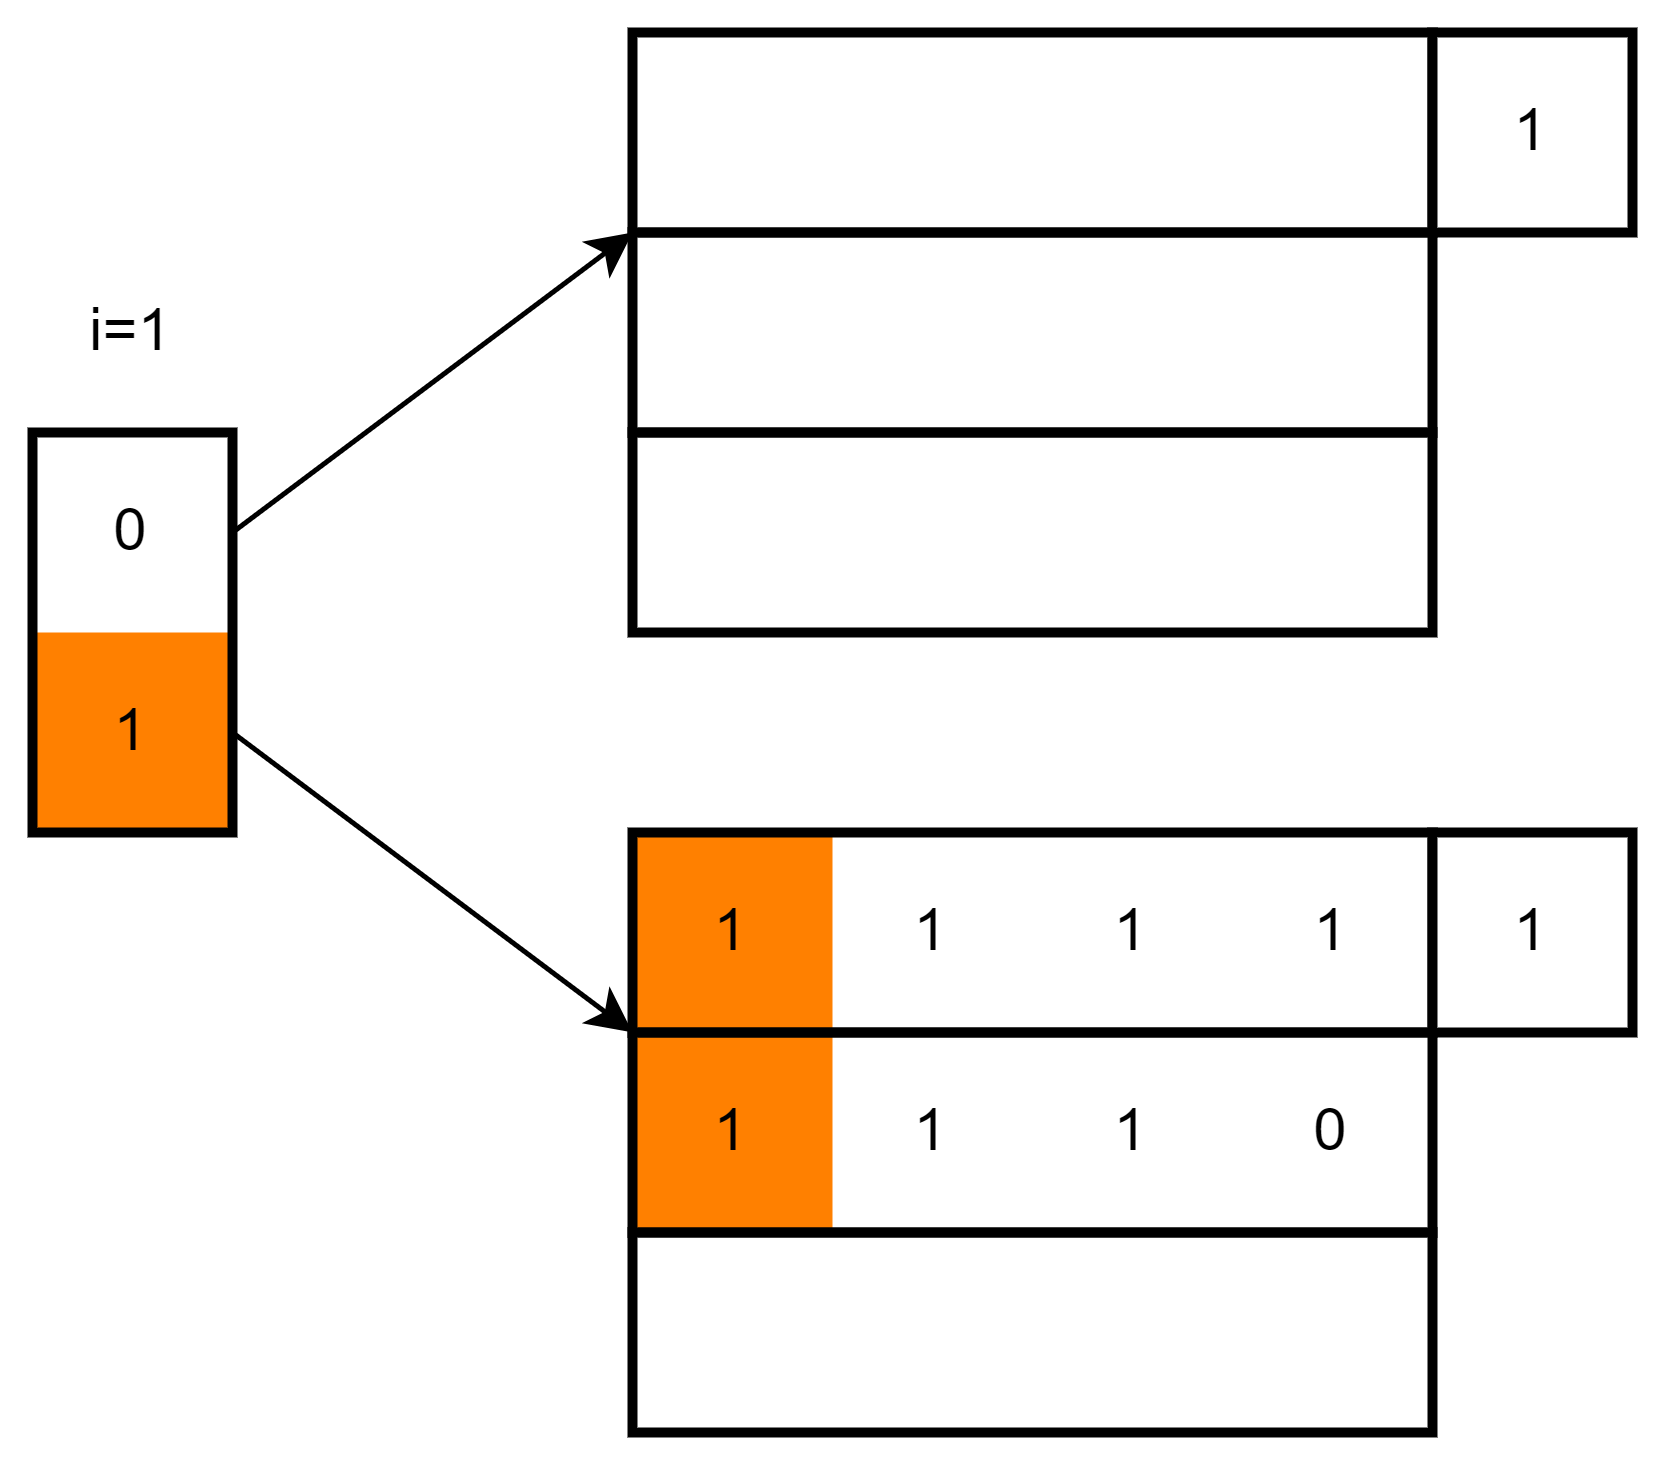
\includegraphics[width=0.4\textwidth]{diagram/Problema2-22.png}
            \end{center}
            Ingresamos 1101:
            \begin{center}
                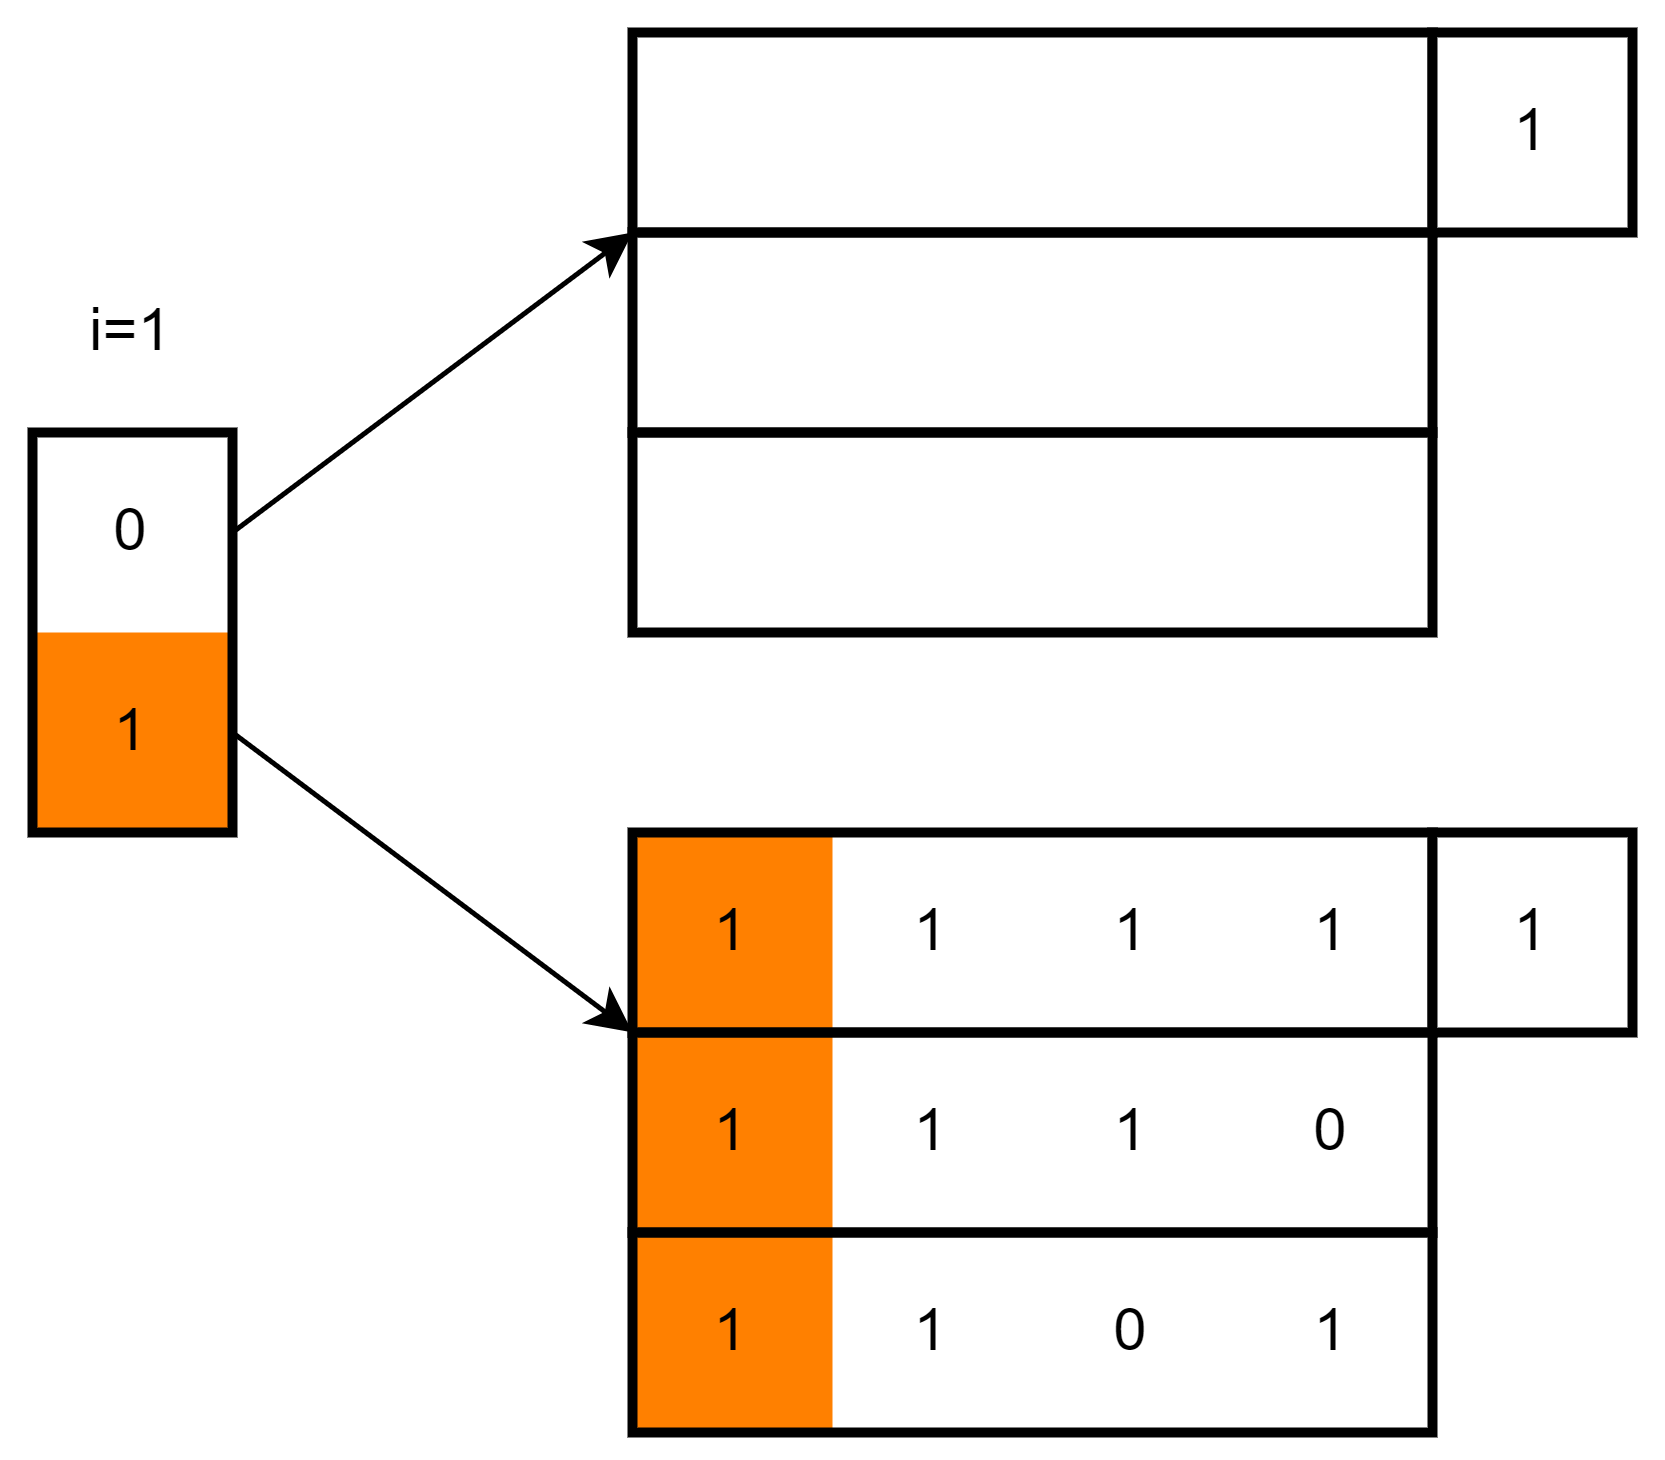
\includegraphics[width=0.4\textwidth]{diagram/Problema2-23.png}
            \end{center}
            \newpage
            Ingresamos 1100: (Al aumentar i a 2, podemos observar que aun no se puede ingresar 1100)
            \begin{center}
                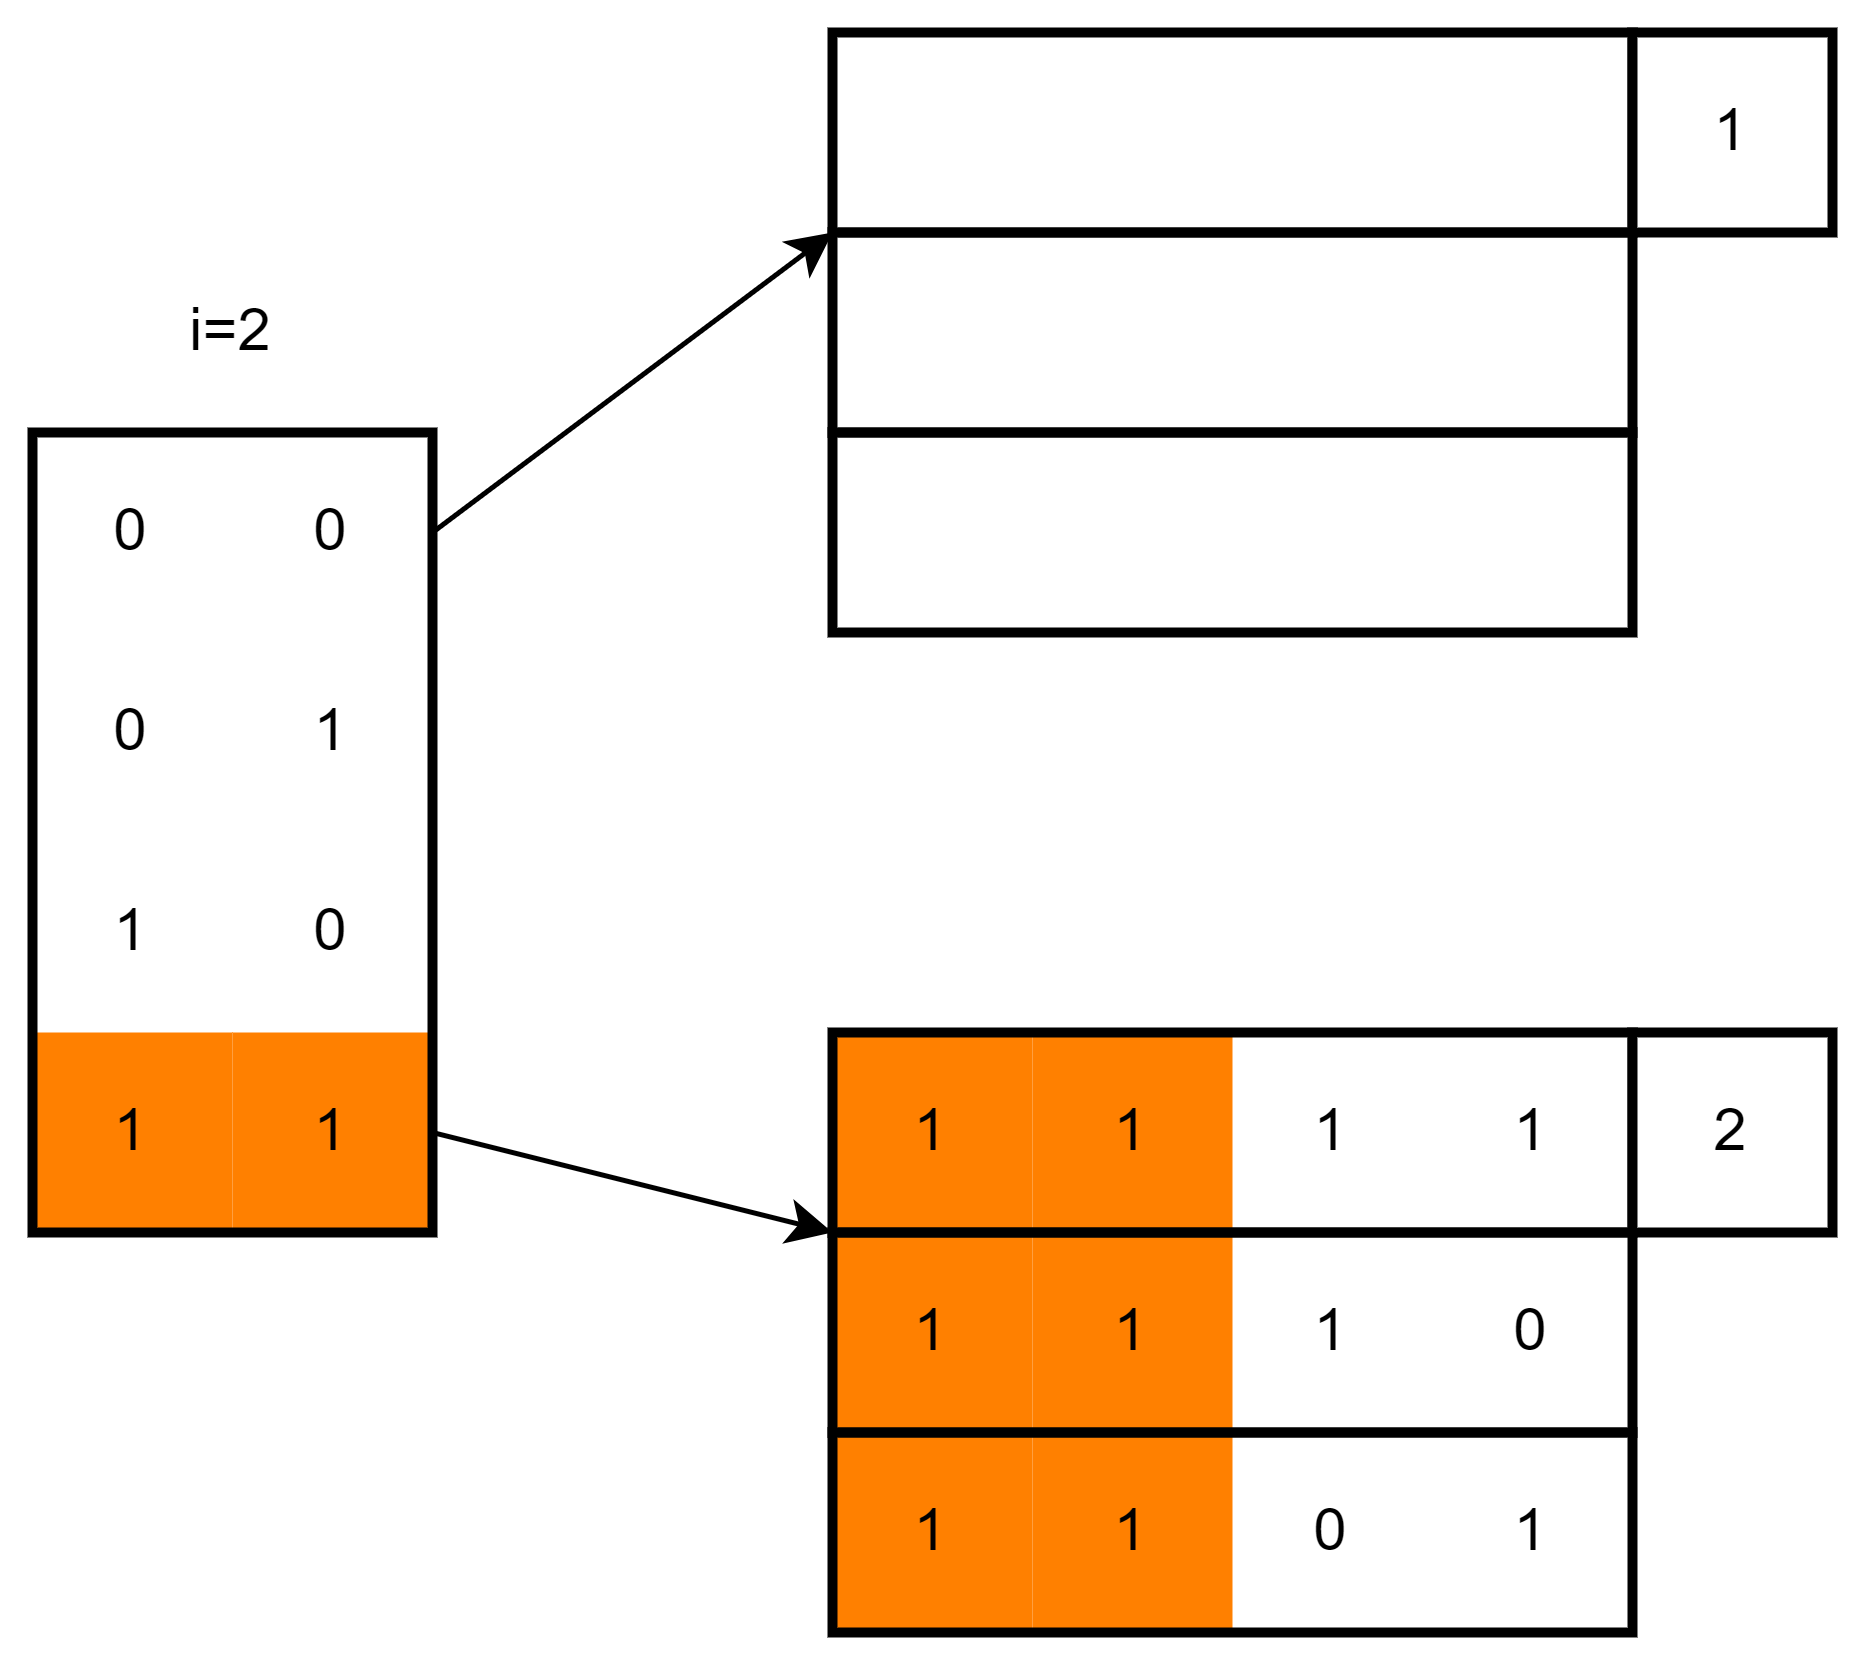
\includegraphics[width=0.4\textwidth]{diagram/Problema2-241.png}
            \end{center}
            Por lo que aumentamos i a 3:
            \begin{center}
                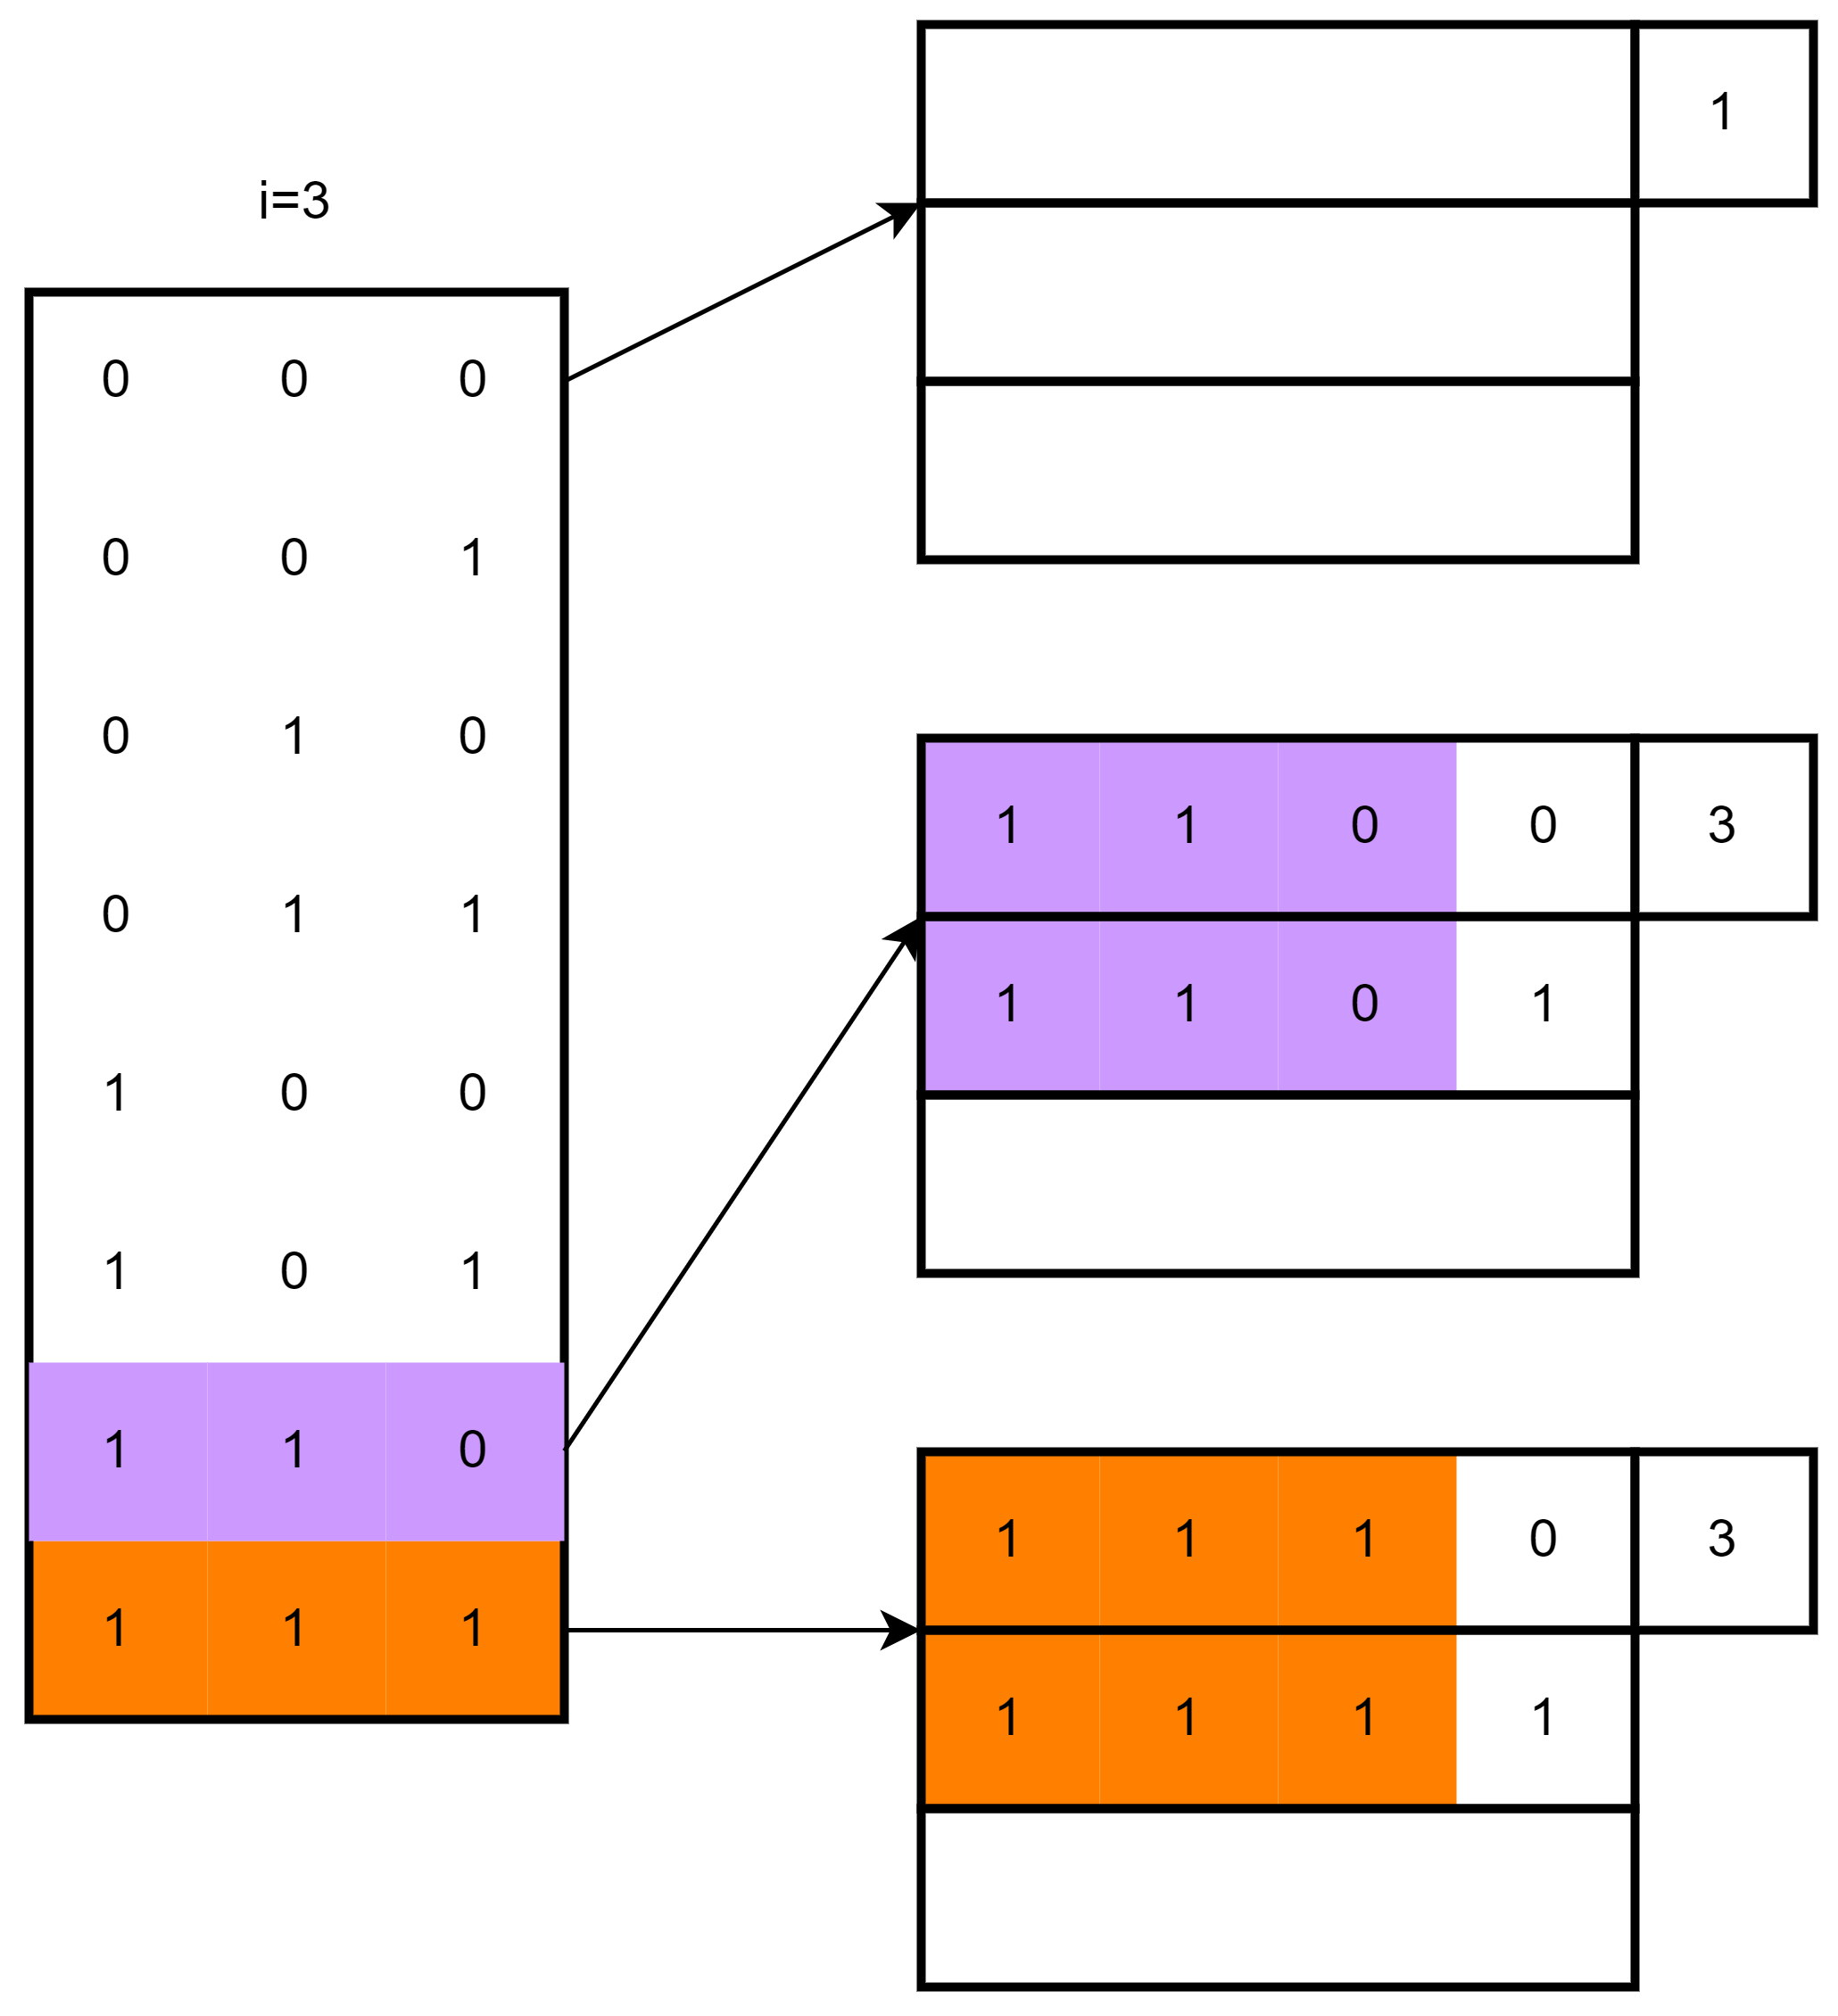
\includegraphics[width=0.4\textwidth]{diagram/Problema2-242.png}
            \end{center}
        }
    \end{enumerate}

    \newpage
    \item \textbf{Pregunta 3:} Considere el siguiente árbol B (figura), inicialmente con el conjunto de claves C cuyo grado mínimo es 3 $(t=3)$.
    \begin{enumerate}
        \item $C = \{20,30,5,18,2,12,15,22,10,1,7,11,31,40,50,35,37,21,23,45,56,57,60\}$.
        \begin{enumerate}
            \renewcommand{\labelenumi}{\alph{enumi})}
            \item Insertar las claves, en el orden en que aparecen las claves en $C$, en el árbol B. Muestre. 
            \begin{enumerate}
                \item Ingresa 20:
                \begin{figure}[H]
                    \centering
                    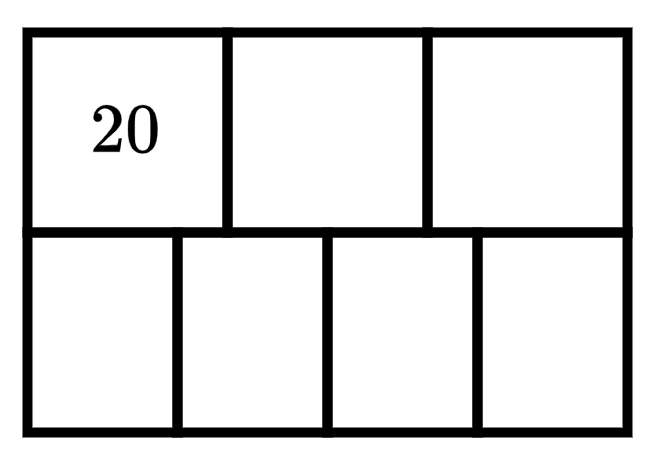
\includegraphics[width=0.2\textwidth]{diagram/P3-1-1.png}
                \end{figure}

                \item Ingresa 30:
                \begin{figure}[H]
                    \centering
                    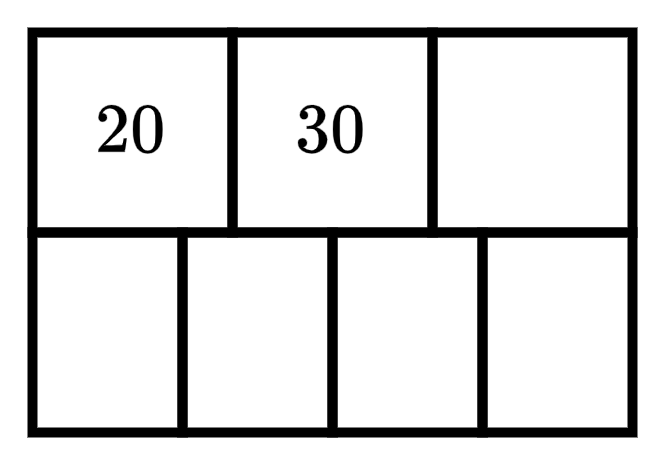
\includegraphics[width=0.2\textwidth]{diagram/P3-1-2.png}
                \end{figure}

                \item Ingresa 5:
                \begin{figure}[H]
                    \centering
                    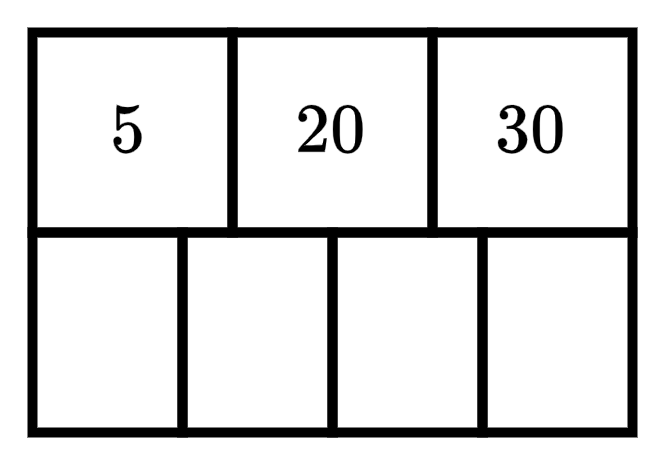
\includegraphics[width=0.2\textwidth]{diagram/P3-1-3.png}
                \end{figure}

                \item Ingresa 18:
                \begin{figure}[H]
                    \centering
                    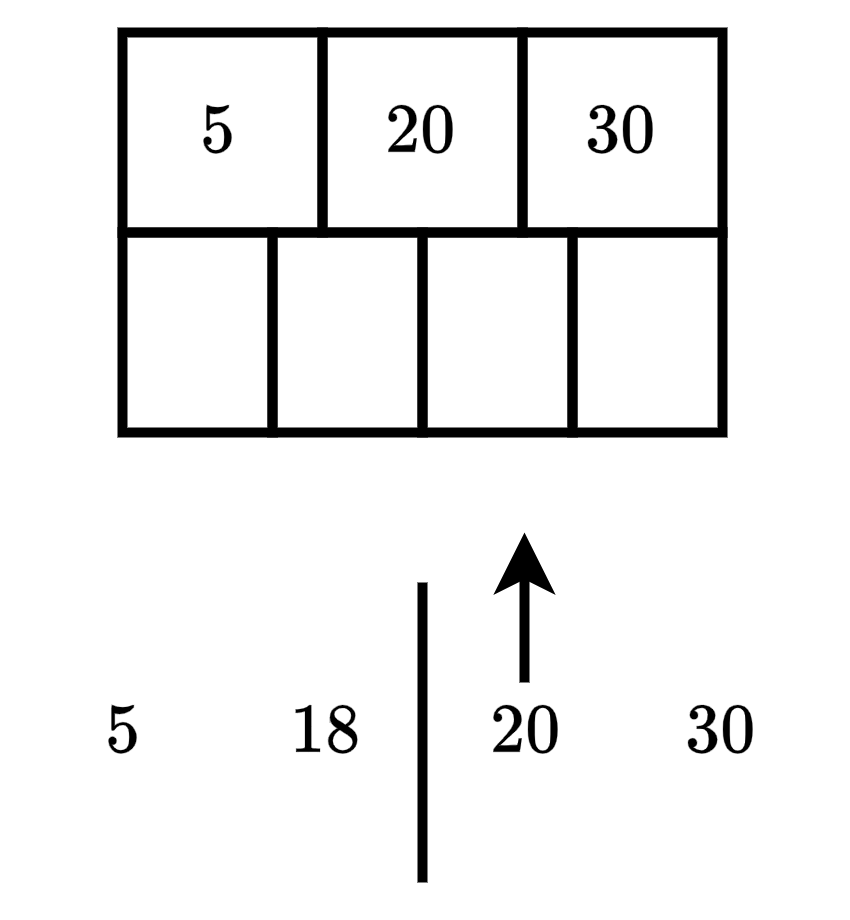
\includegraphics[width=0.22\textwidth]{diagram/P3-1-4-1.png}
                    \rule{\textwidth}{1pt}
                    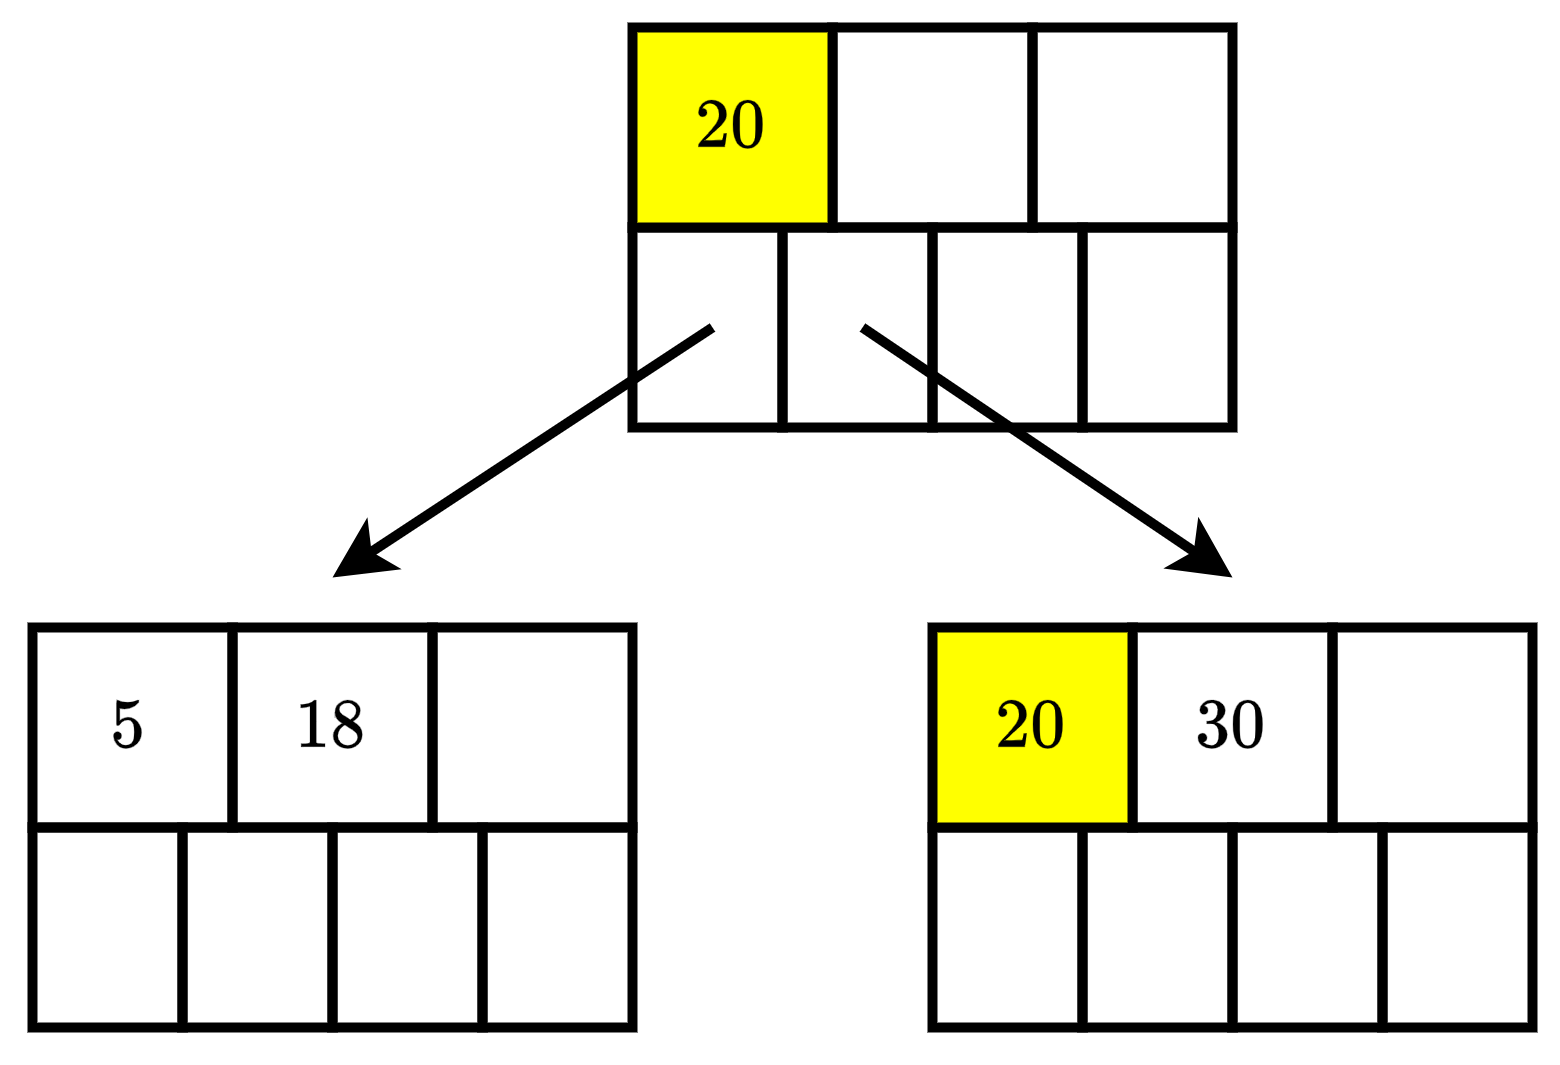
\includegraphics[width=0.40\textwidth]{diagram/P3-1-4-2.png}
                \end{figure}

                \newpage
                \item Ingresa 2:
                \begin{figure}[H]
                    \centering
                    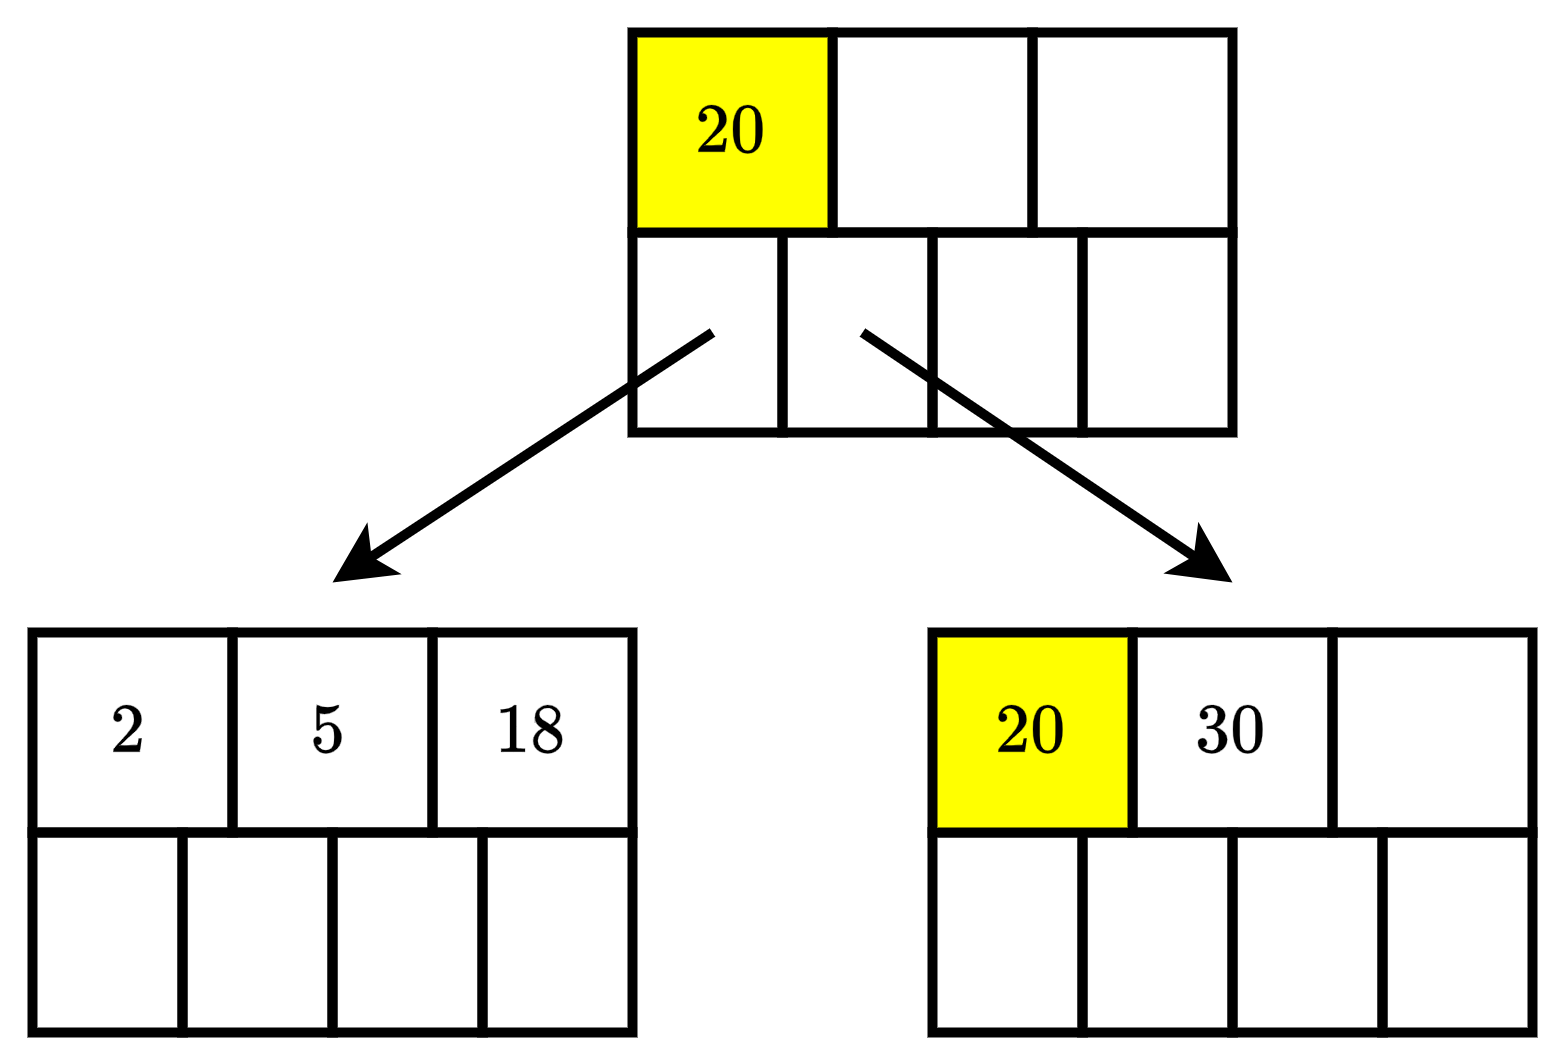
\includegraphics[width=0.45\textwidth]{diagram/P3-1-5.png}
                \end{figure}

                \item Ingresa 12:
                \begin{figure}[H]
                    \centering
                    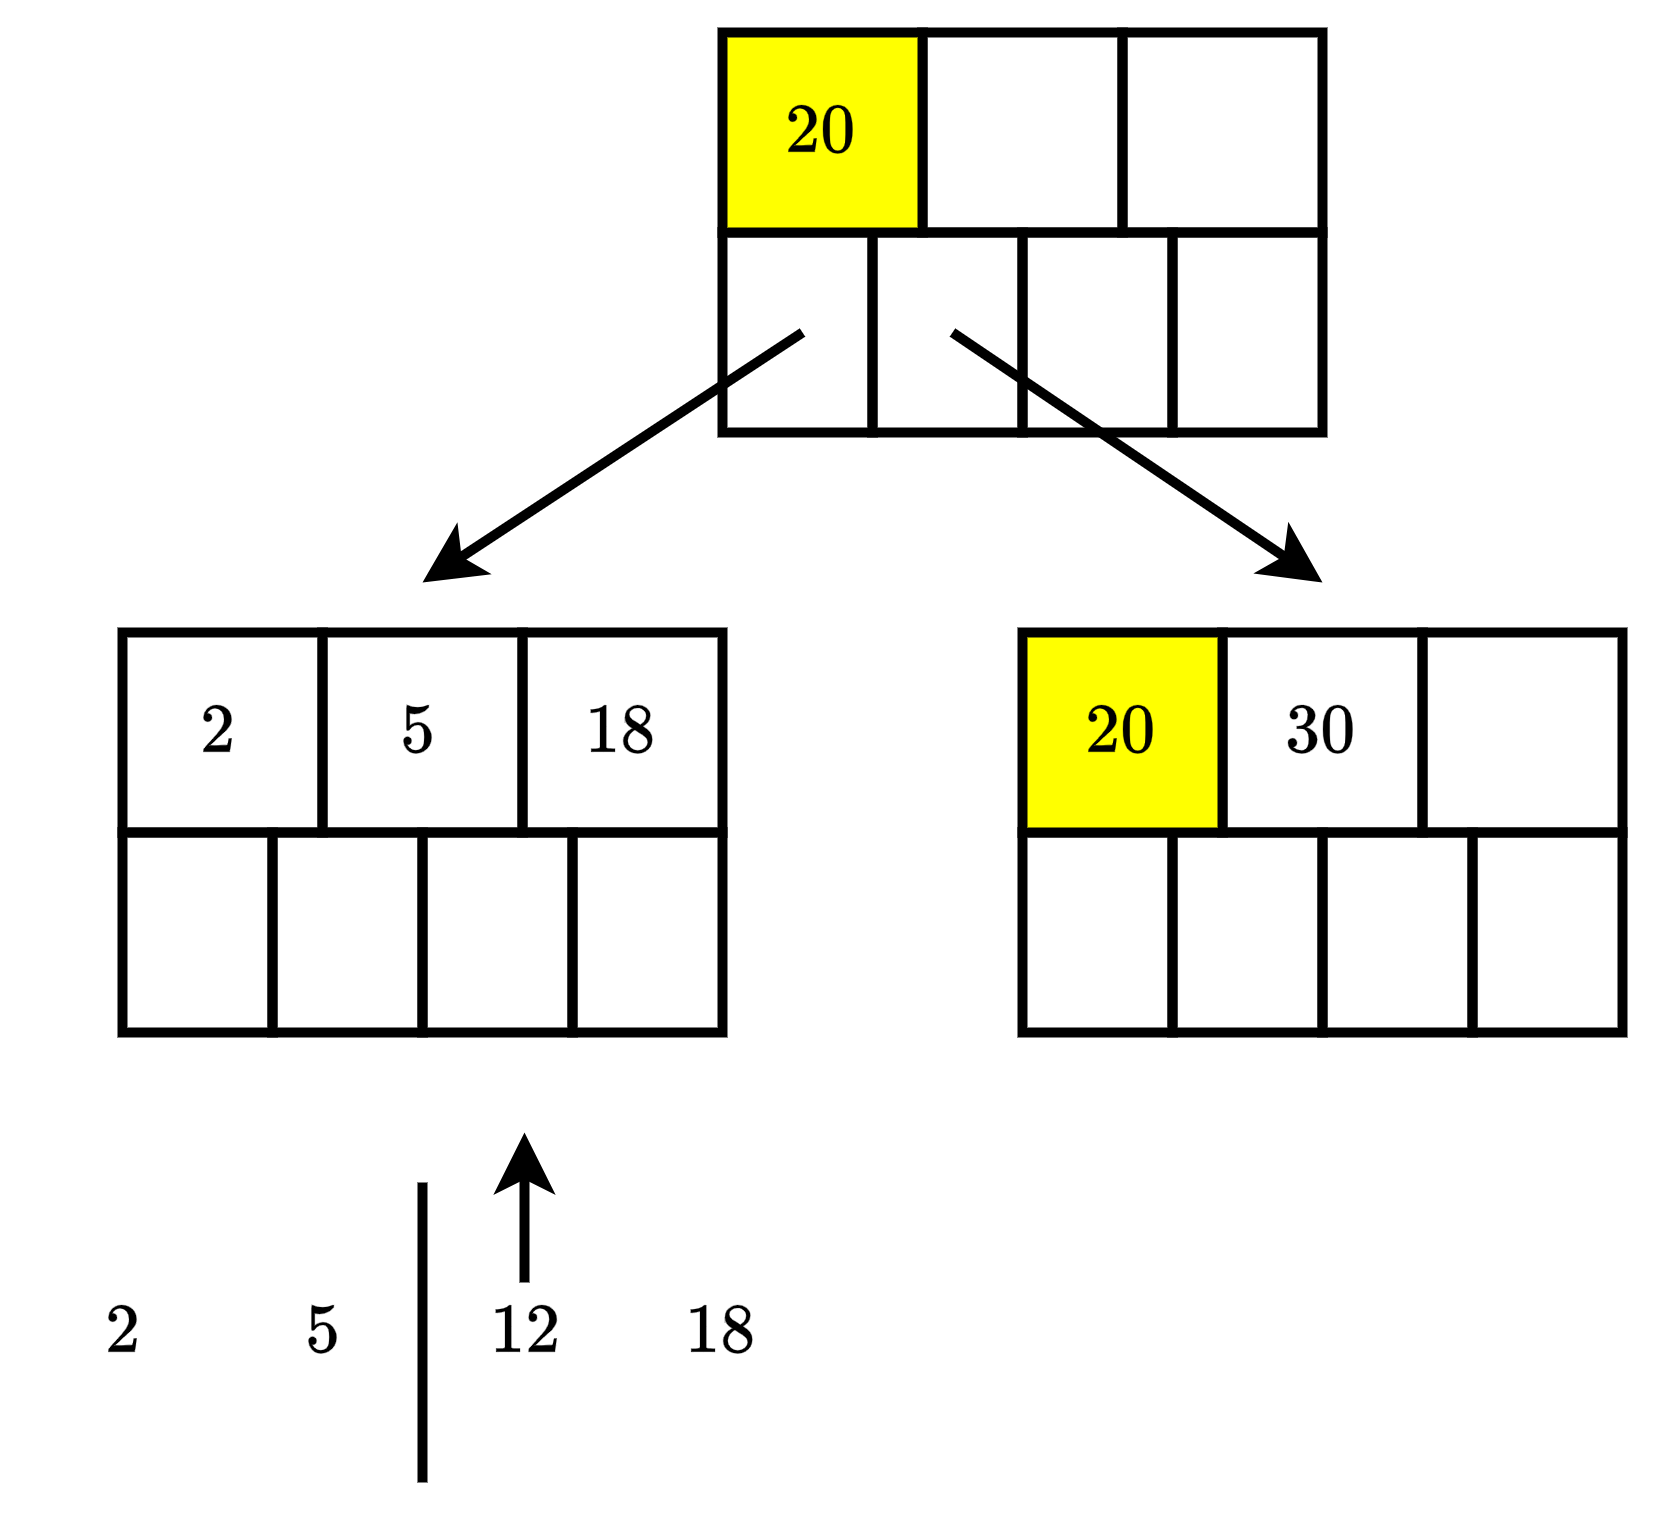
\includegraphics[width=0.45\textwidth]{diagram/P3-1-6-1.png}
                    \rule{\textwidth}{1pt}
                    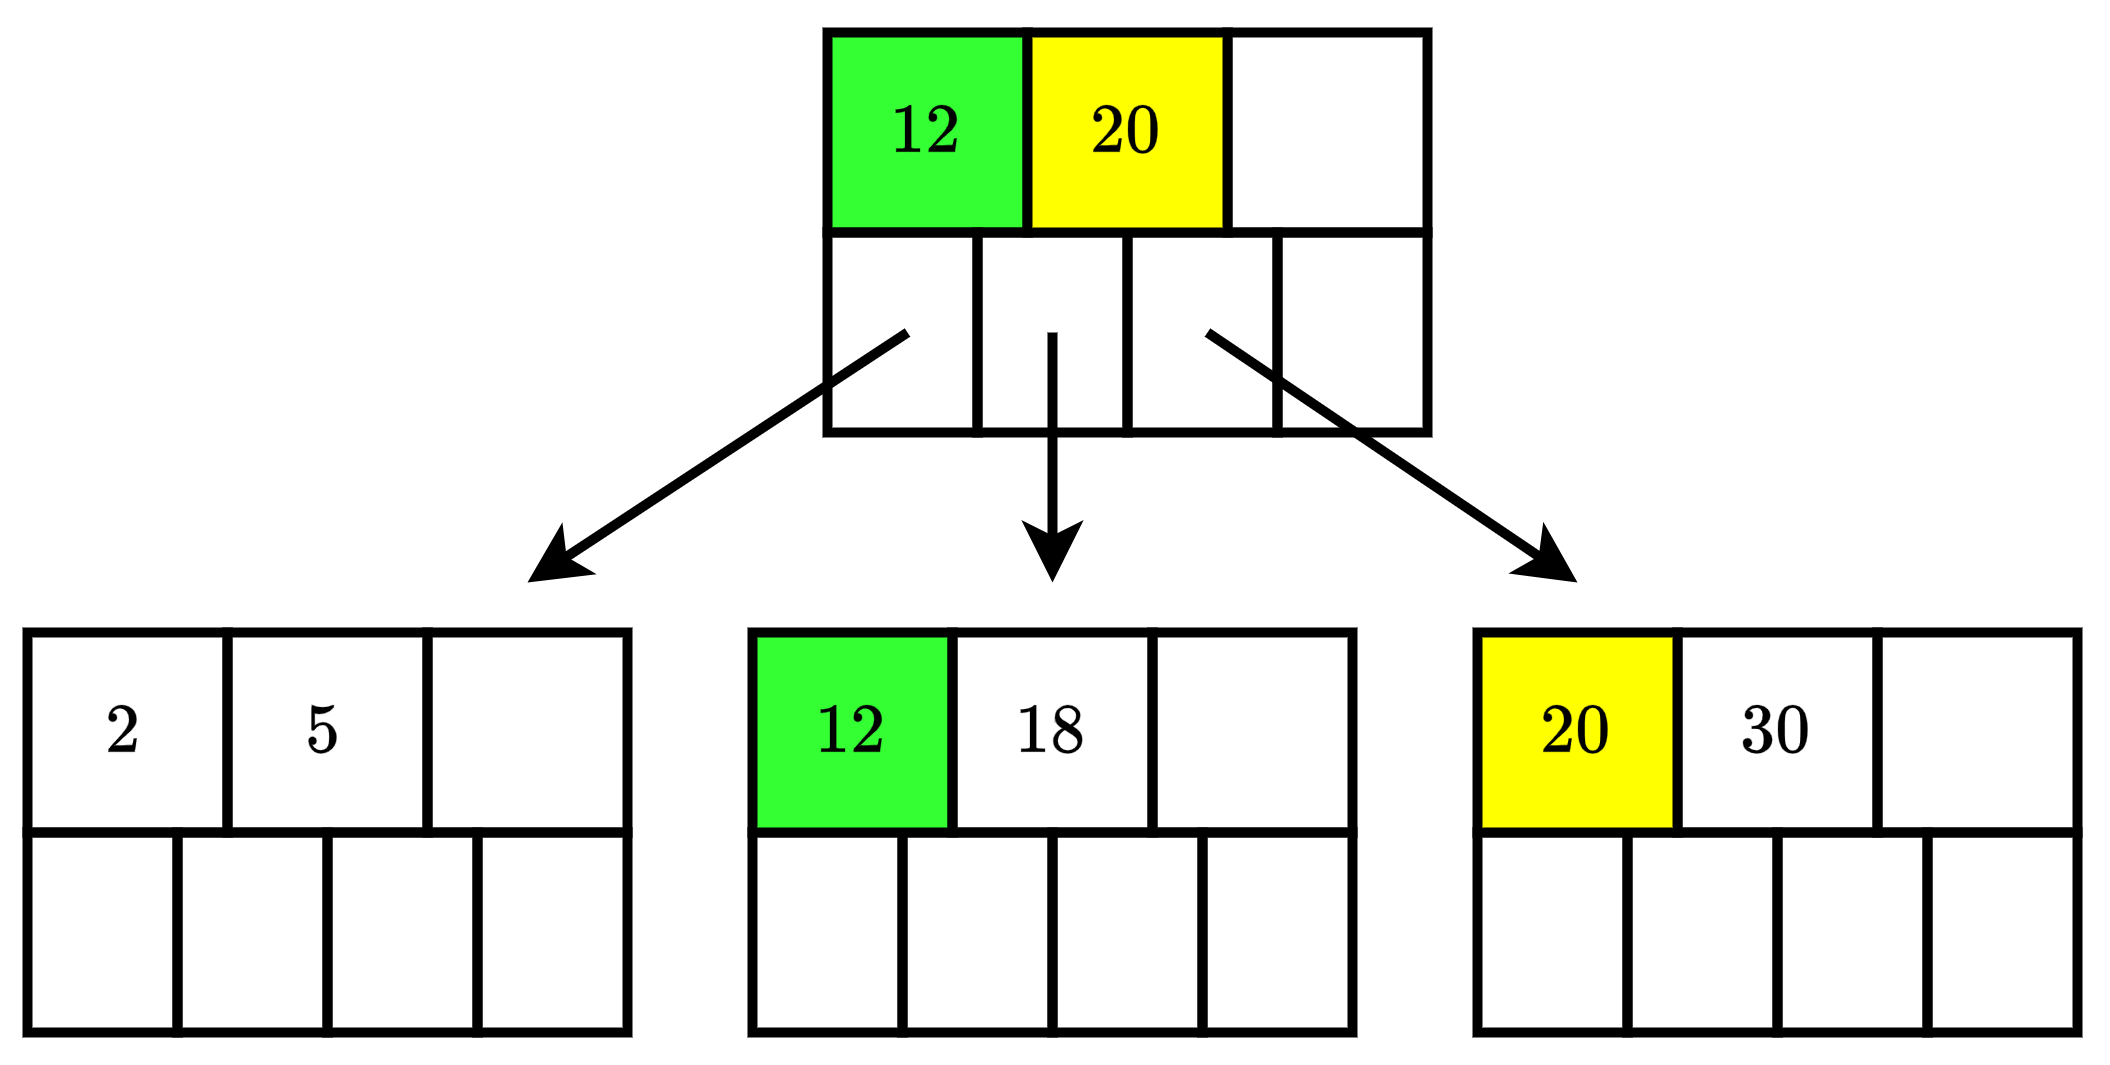
\includegraphics[width=0.6\textwidth]{diagram/P3-1-6-2.png}
                \end{figure}

                \newpage
                \item Ingresa 15:
                \begin{figure}[H]
                    \centering
                    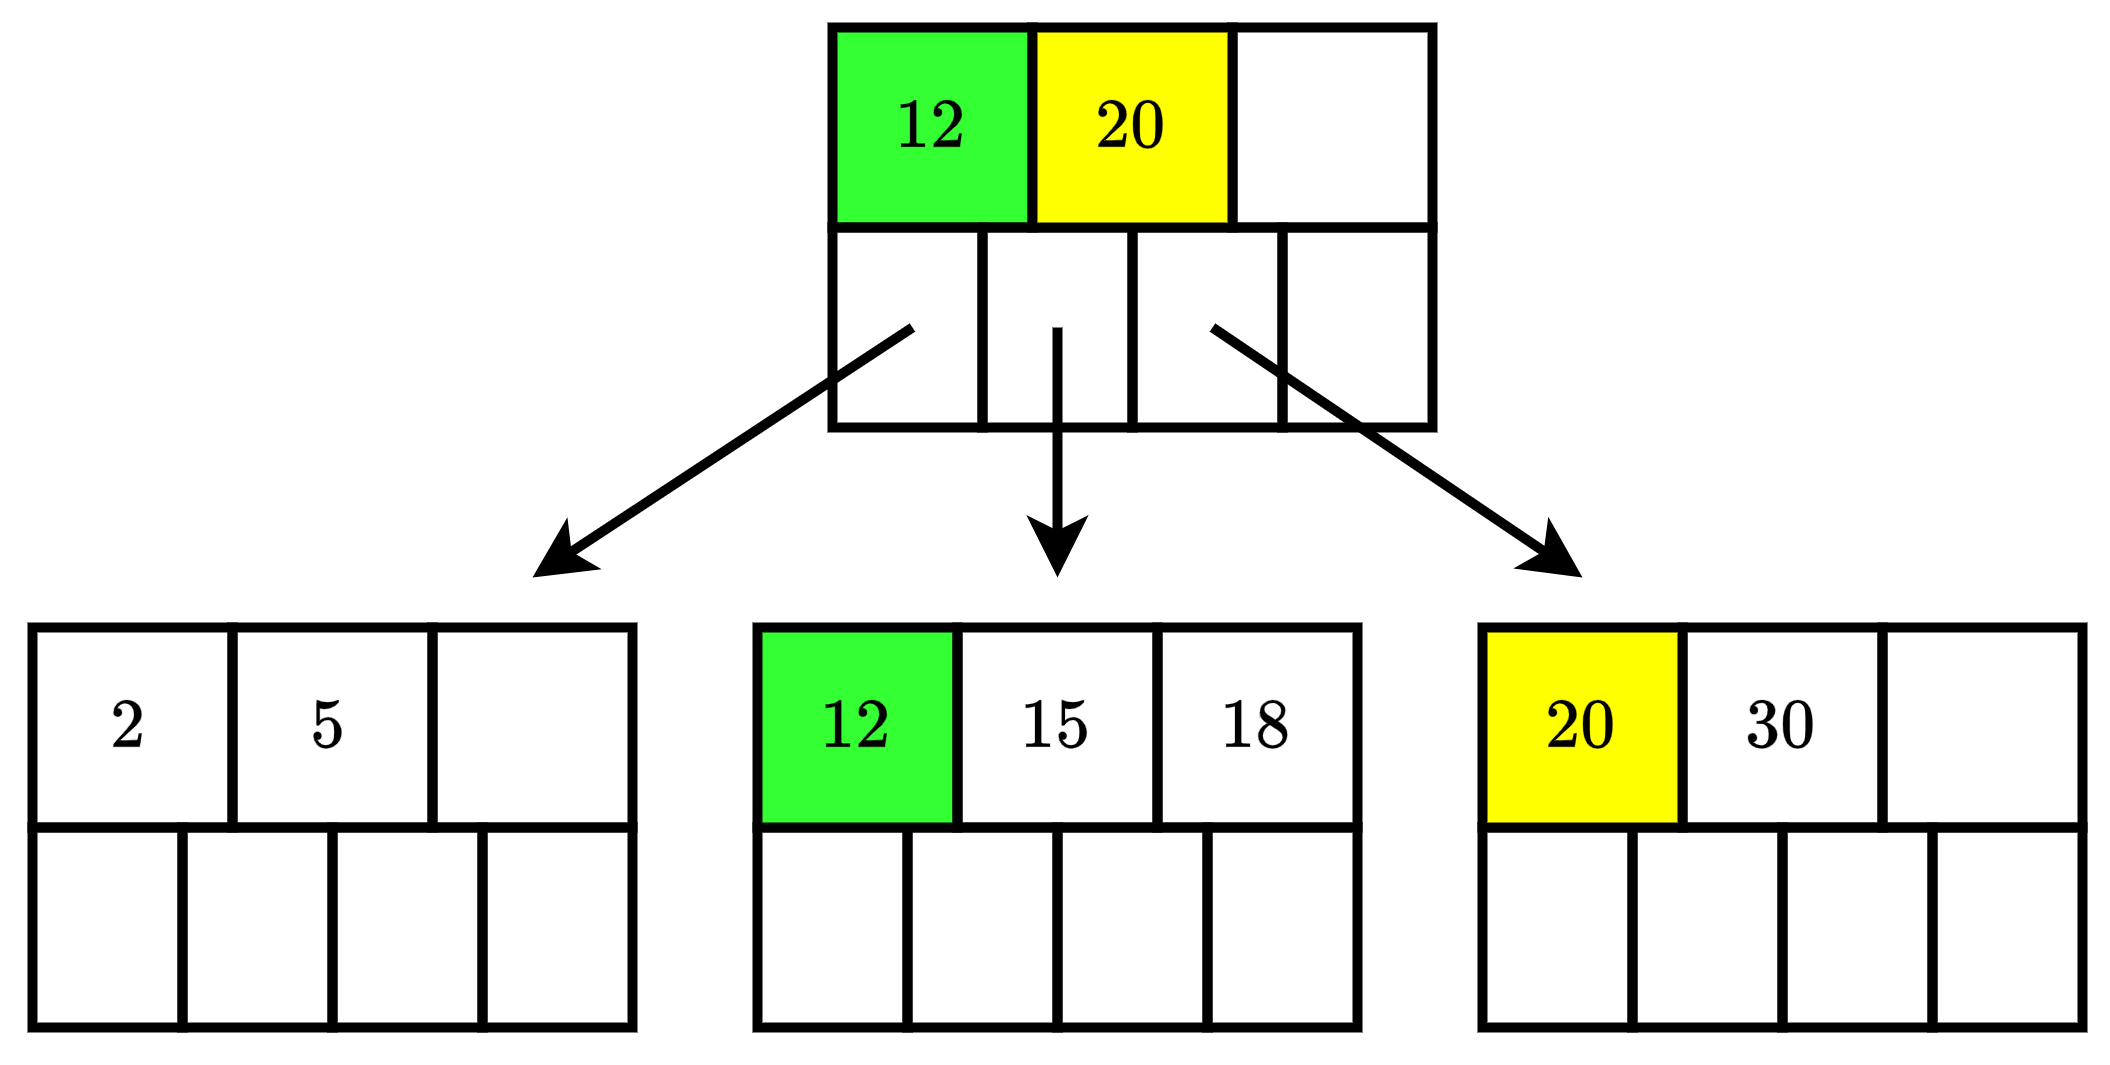
\includegraphics[width=0.6\textwidth]{diagram/P3-1-7.png}
                \end{figure}

                \item Ingresa 22:
                \begin{figure}[H]
                    \centering
                    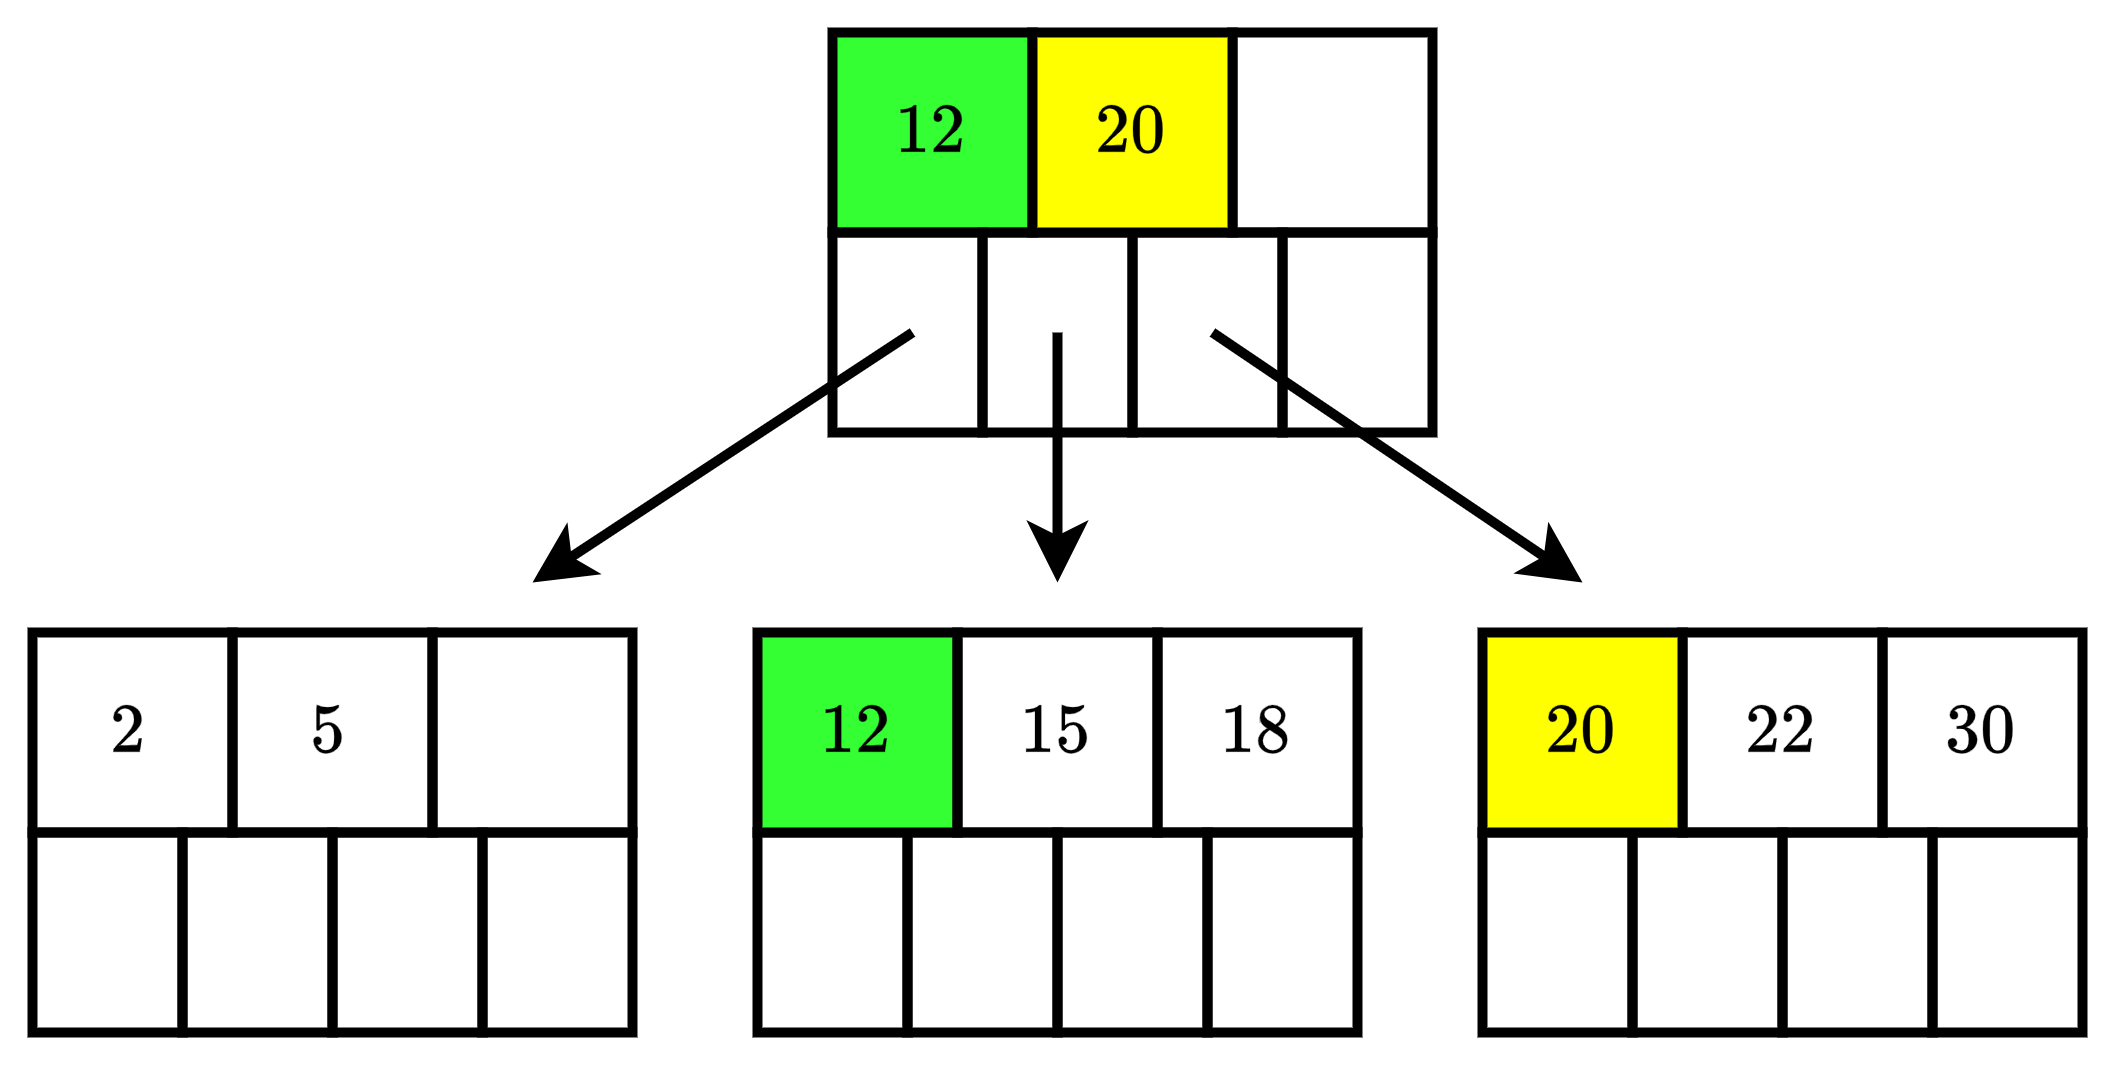
\includegraphics[width=0.6\textwidth]{diagram/P3-1-8.png}
                \end{figure}

                \item Ingresa 10:
                \begin{figure}[H]
                    \centering
                    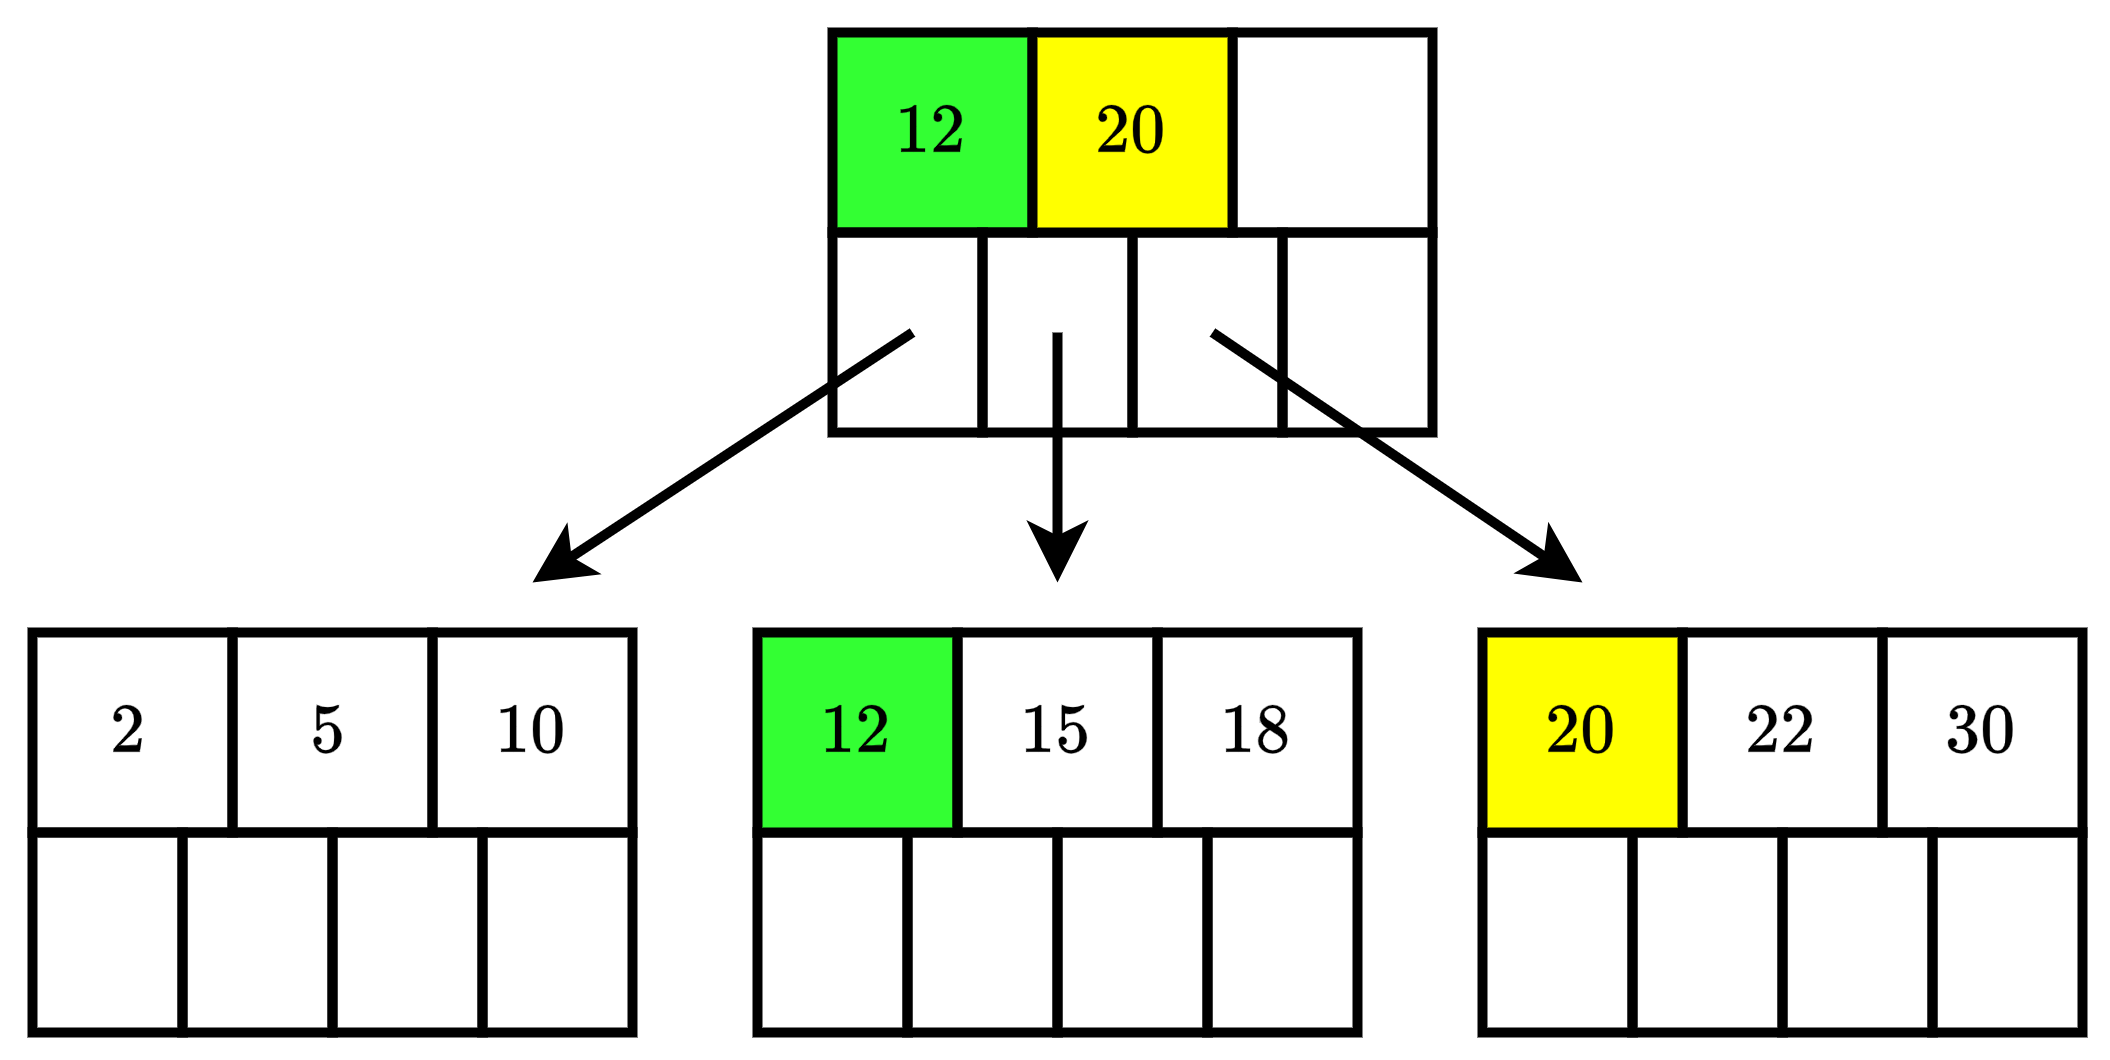
\includegraphics[width=0.6\textwidth]{diagram/P3-1-9.png}
                \end{figure}

                \newpage
                \item Ingresa 1:
                \begin{figure}[H]
                    \centering
                    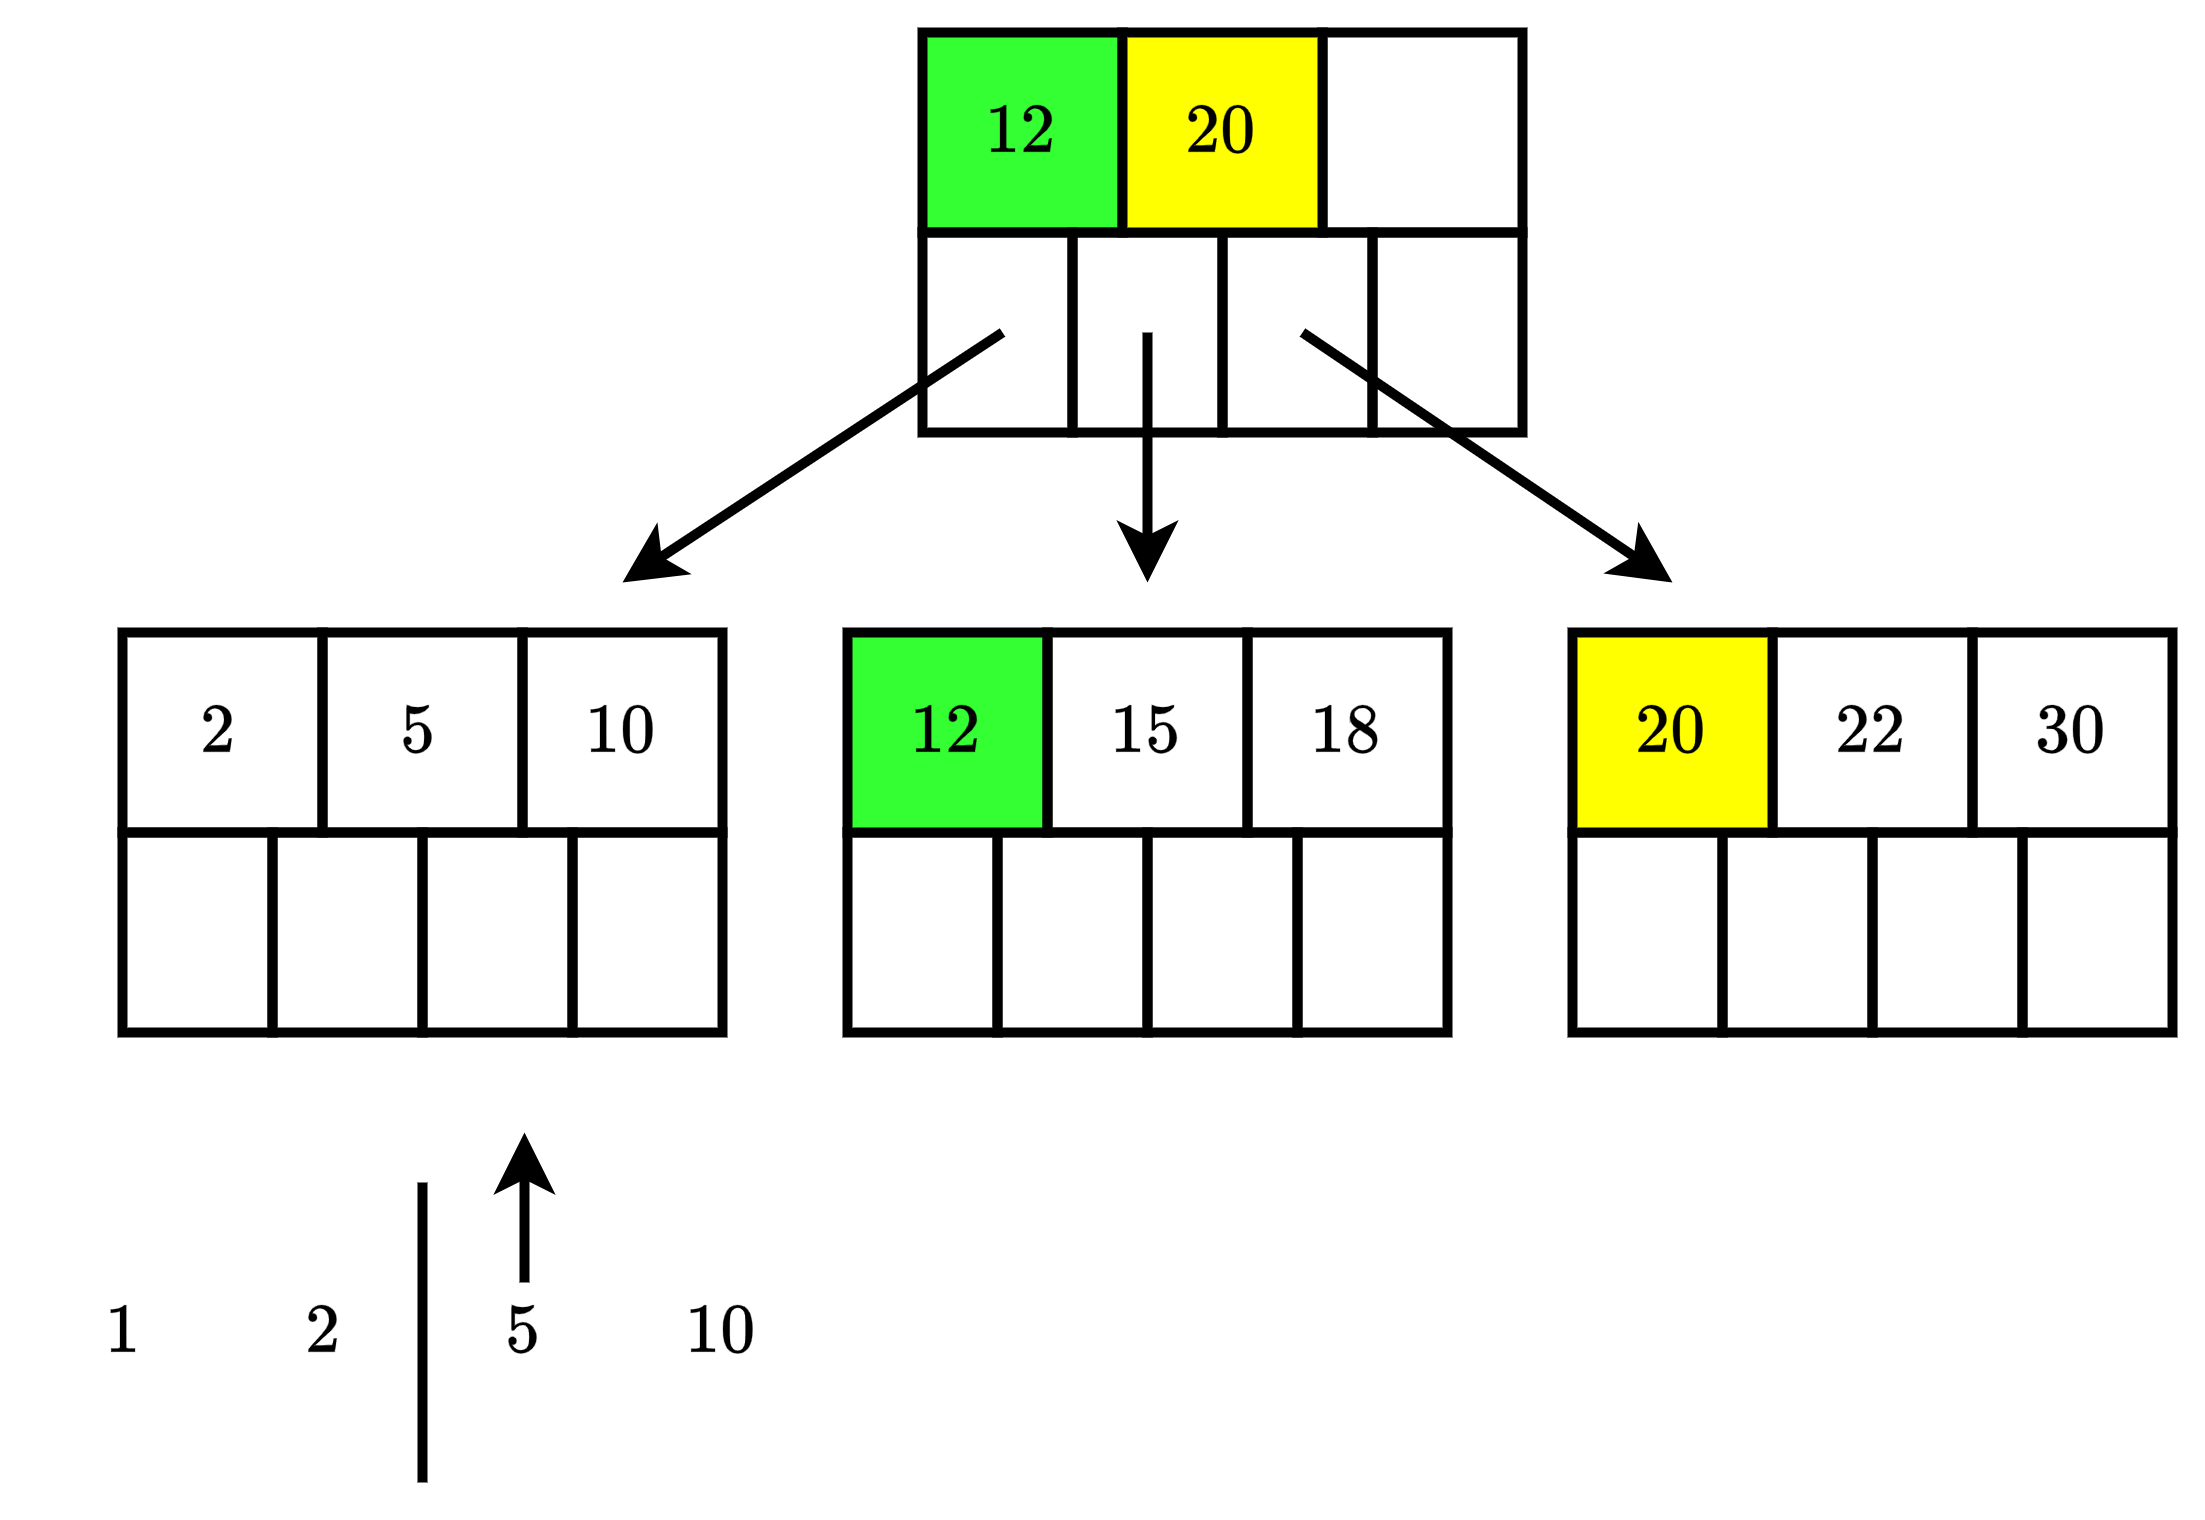
\includegraphics[width=0.6\textwidth]{diagram/P3-1-10-1.png}
                    \rule{\textwidth}{1pt}
                    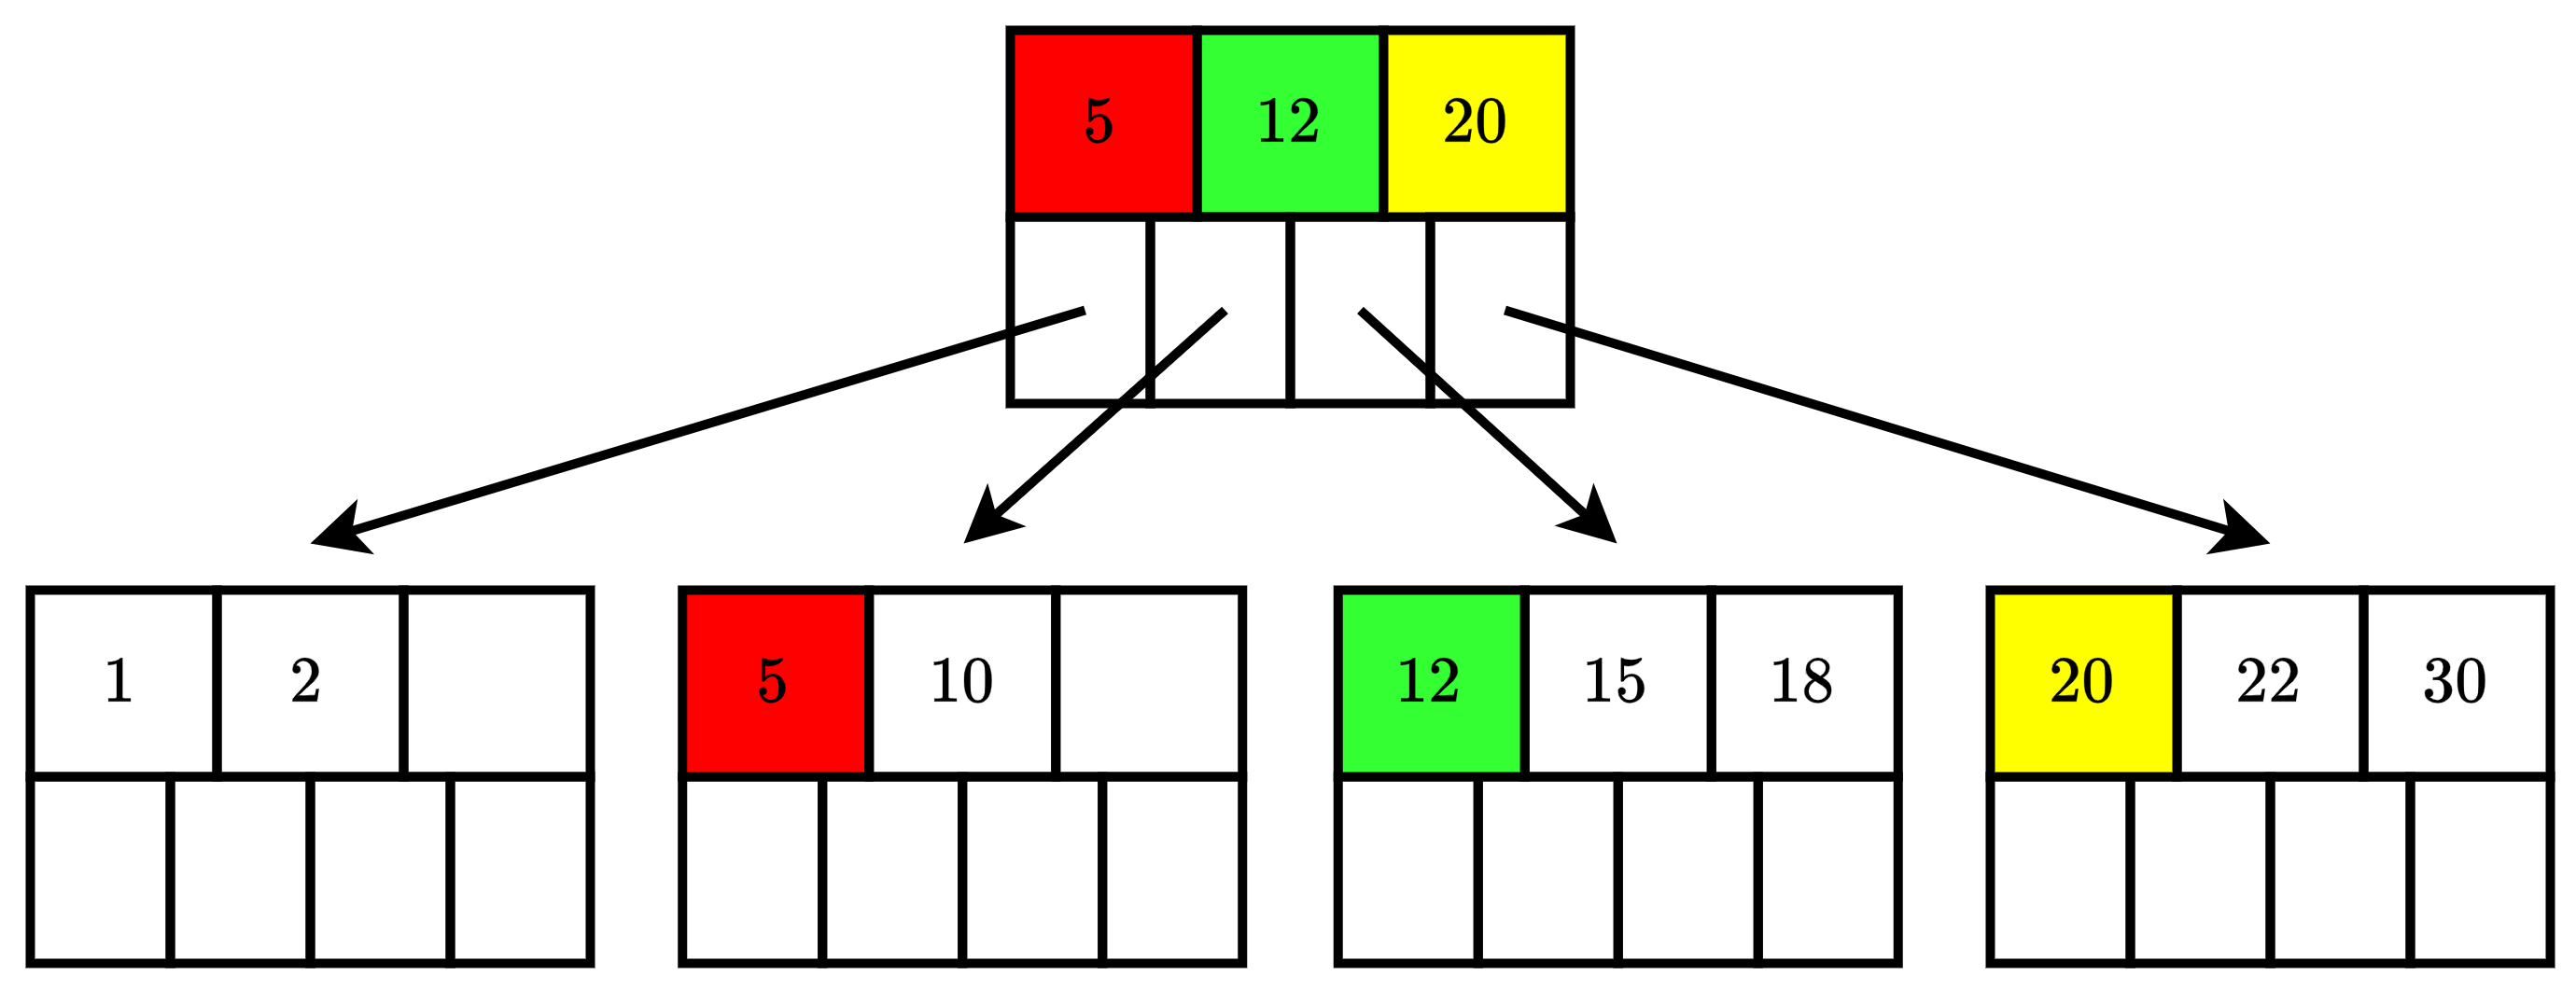
\includegraphics[width=0.7\textwidth]{diagram/P3-1-10-2.png}
                \end{figure}

                \item Ingresa 7:
                \begin{figure}[H]
                    \centering
                    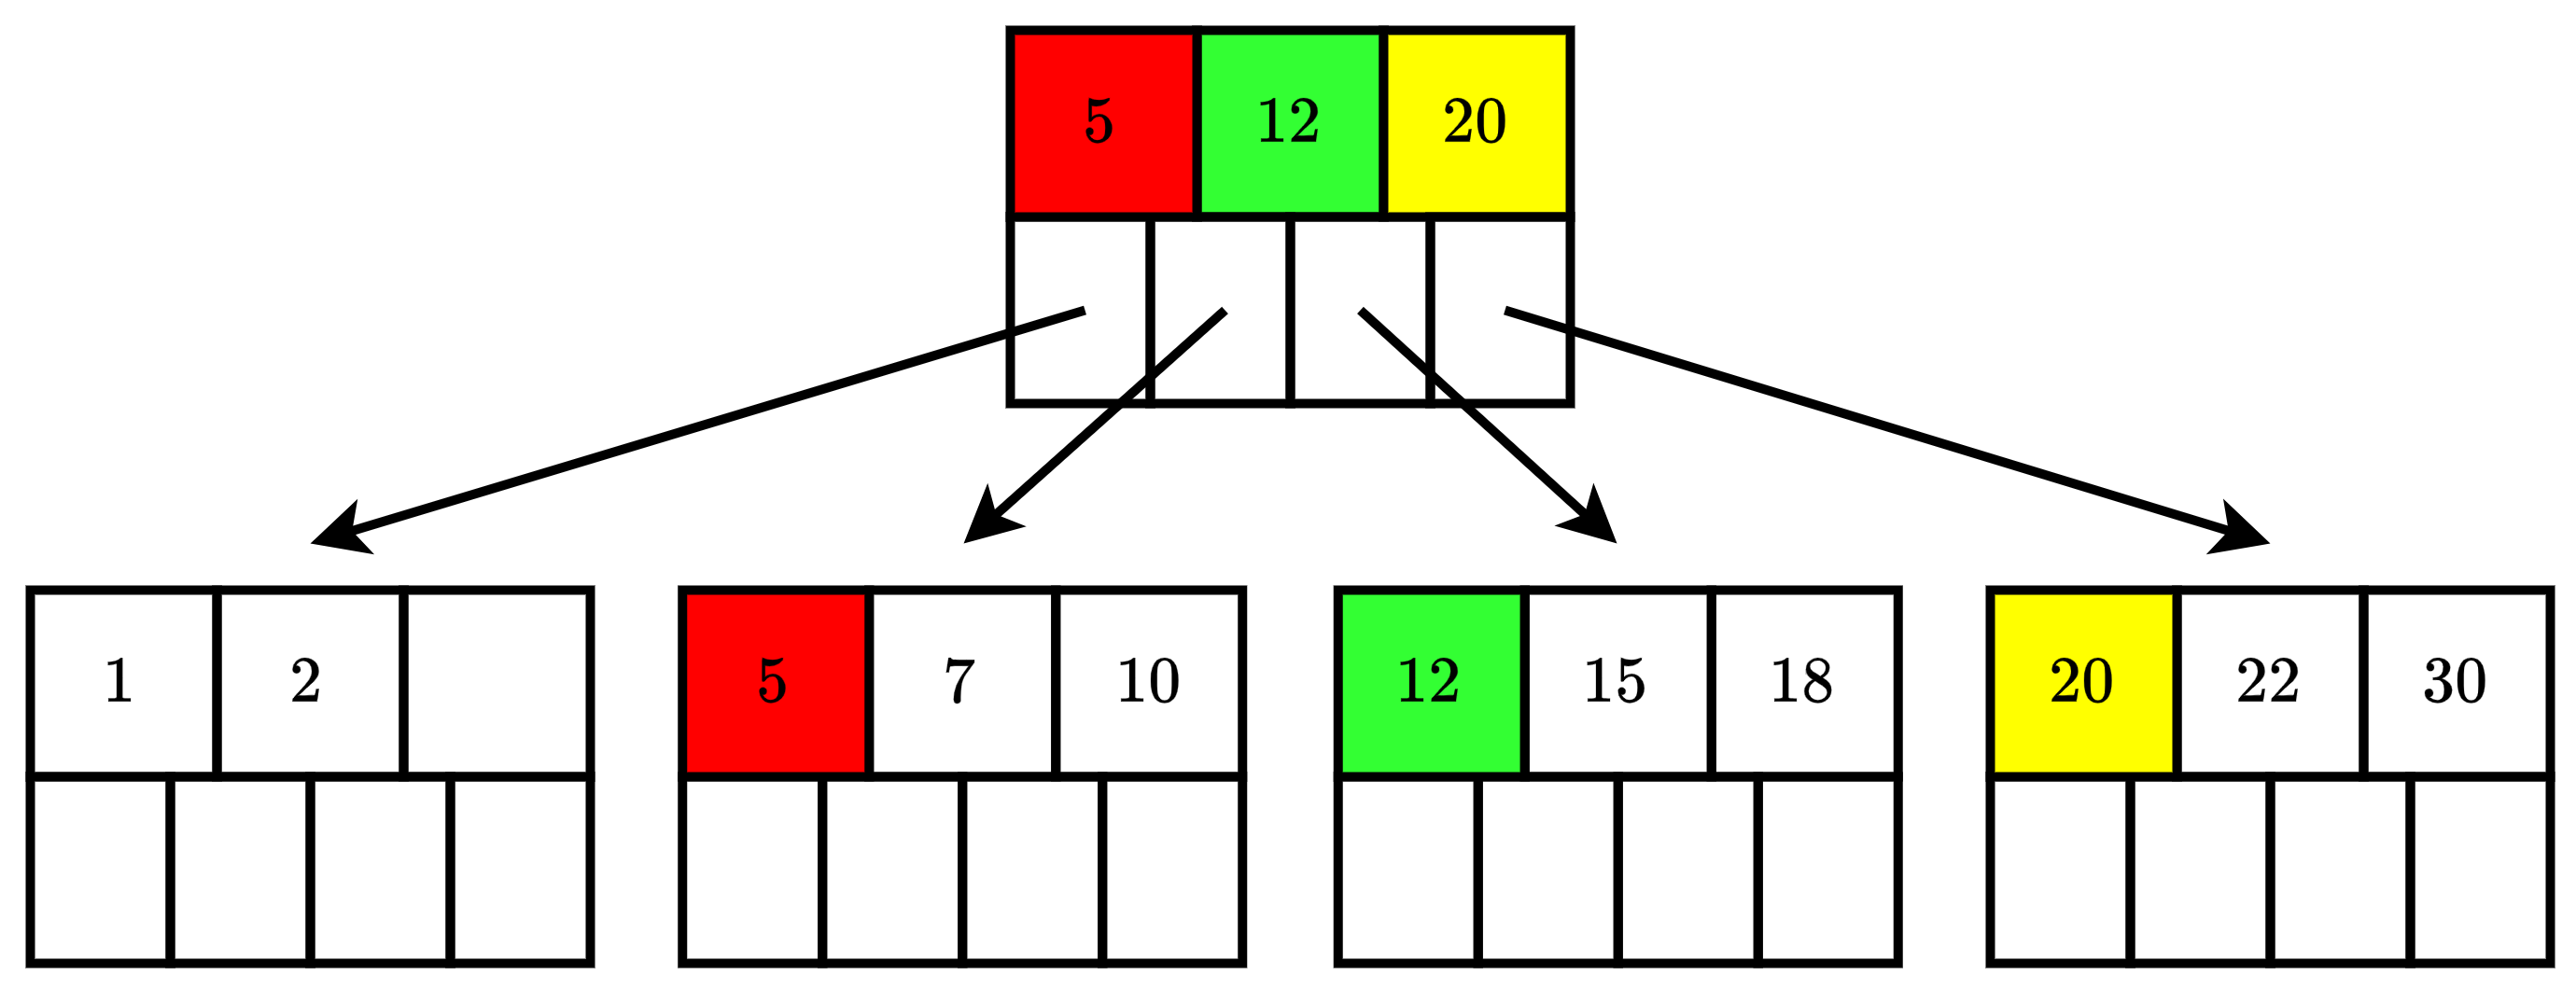
\includegraphics[width=0.6\textwidth]{diagram/P3-1-11.png}
                \end{figure}

                \newpage
                \item Ingresa 11:
                \begin{figure}[H]
                    \centering
                    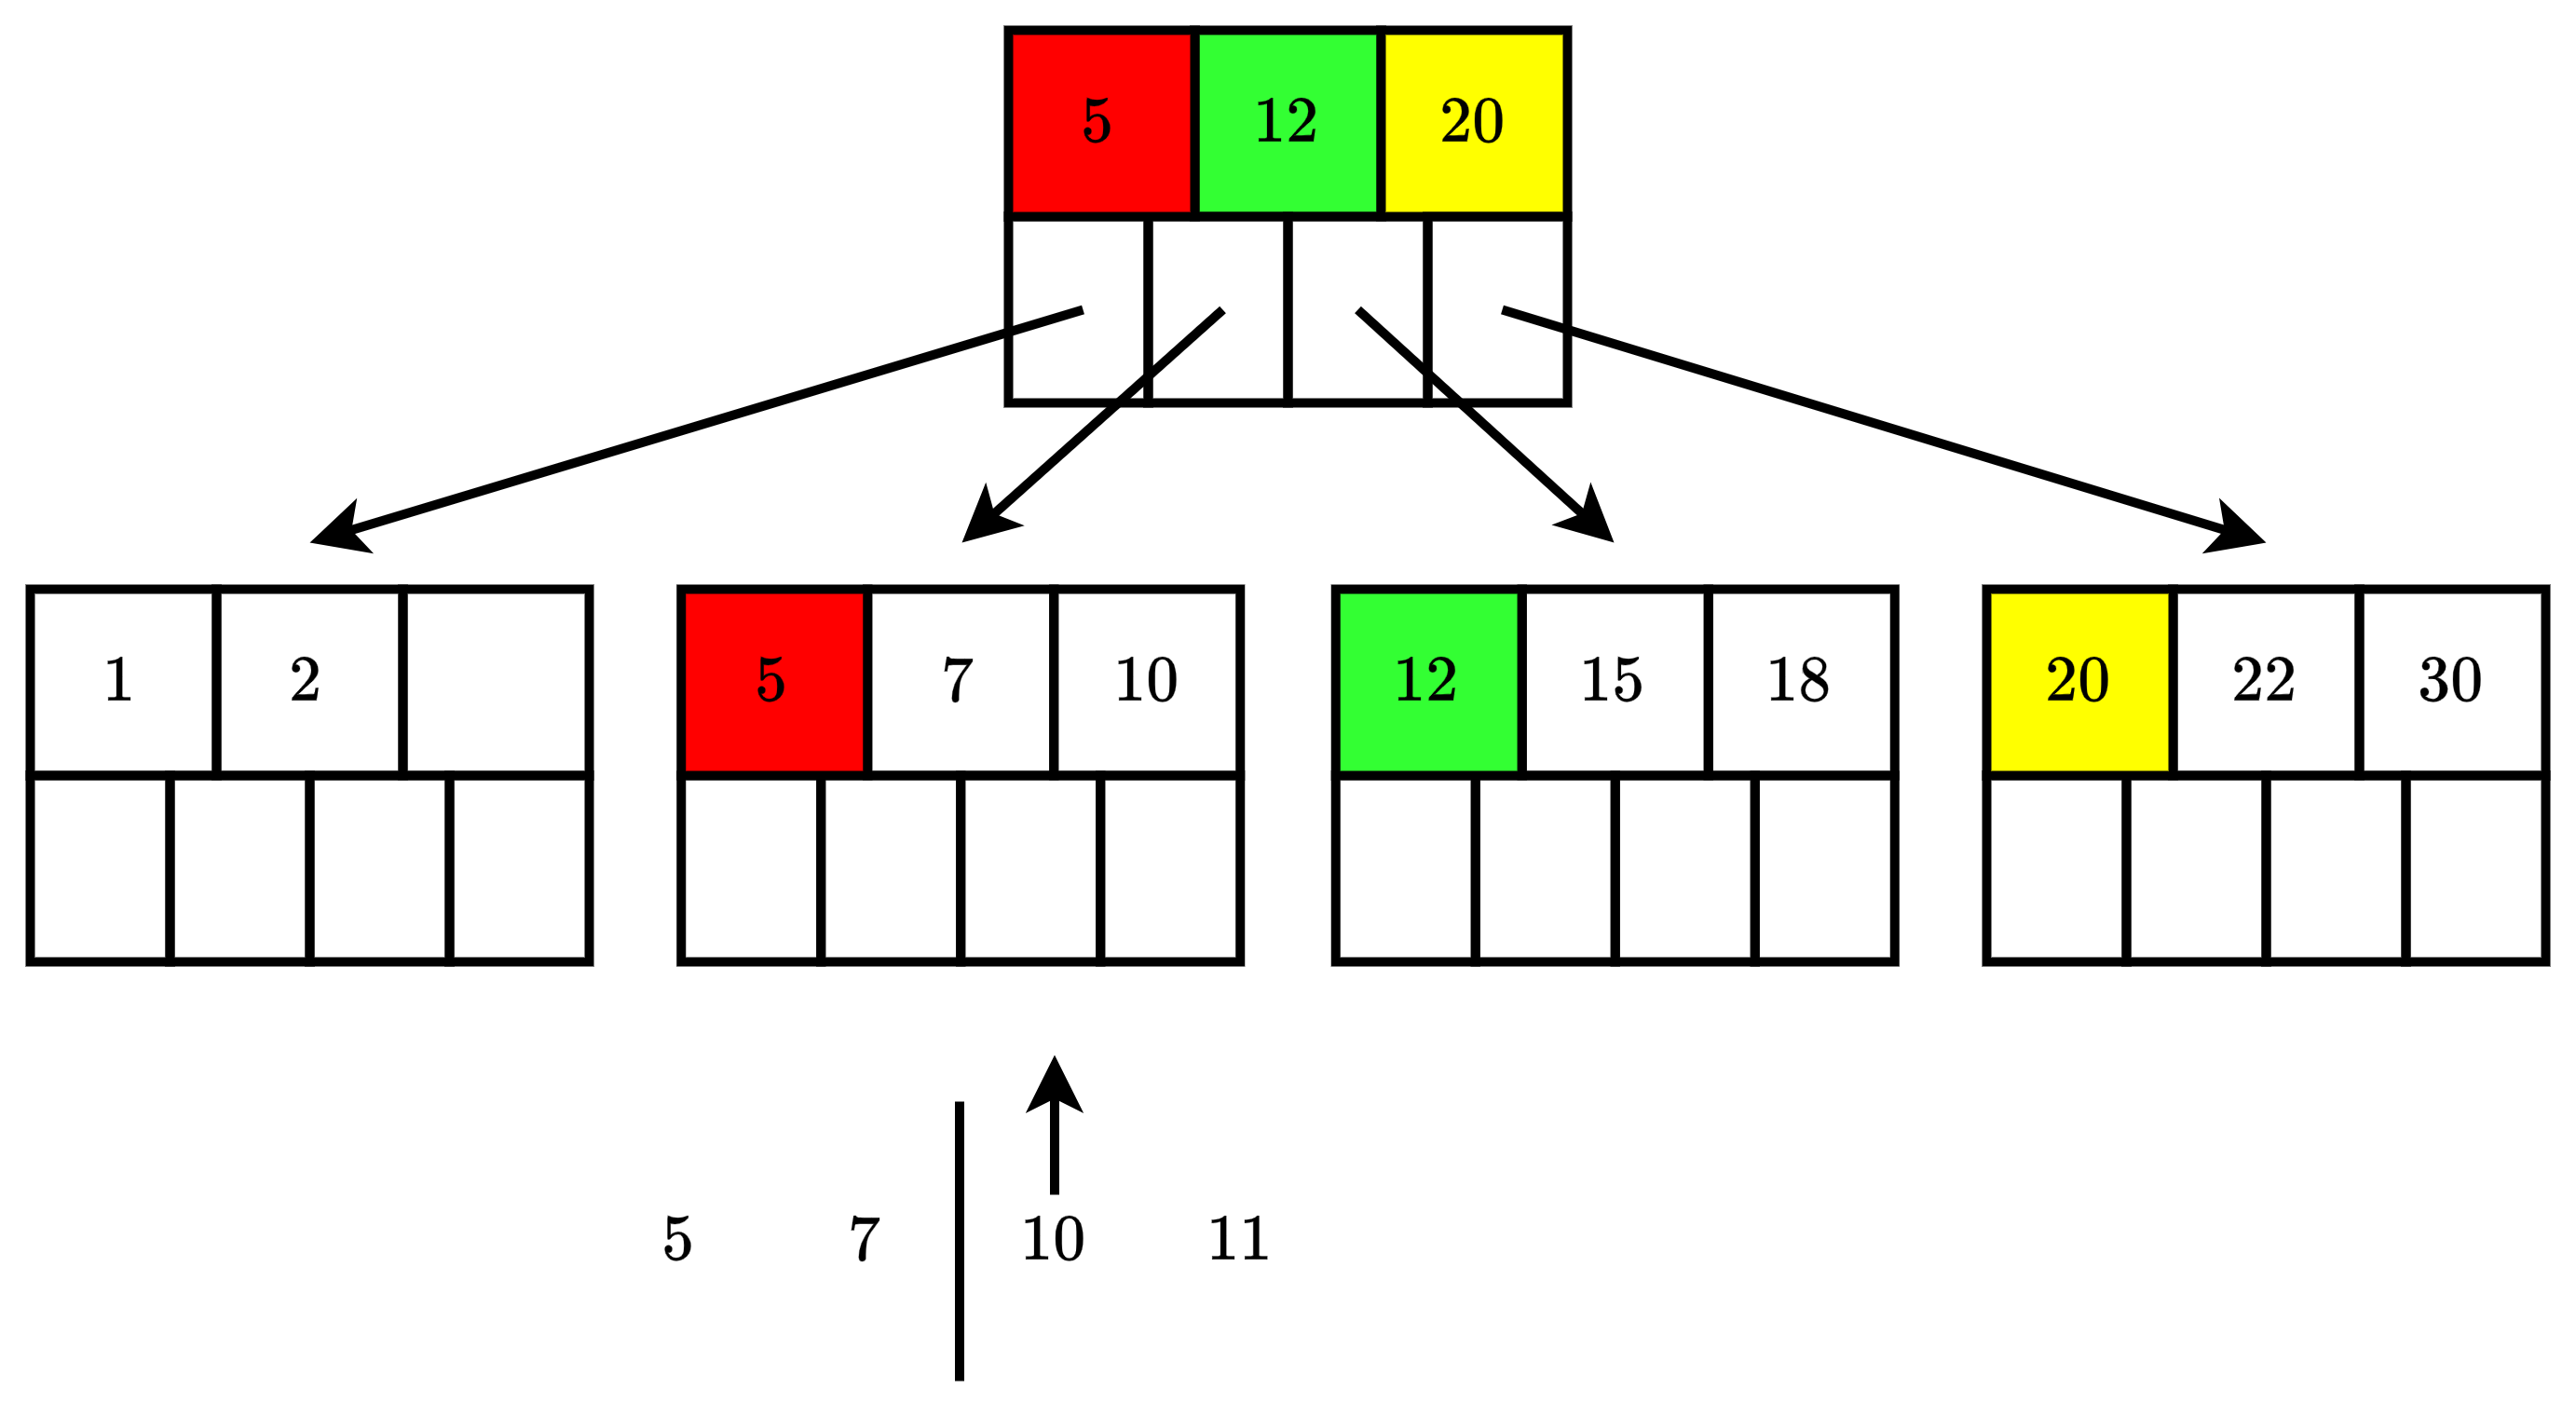
\includegraphics[width=0.6\textwidth]{diagram/P3-1-12-1.png}
                    \rule{\textwidth}{1pt}
                    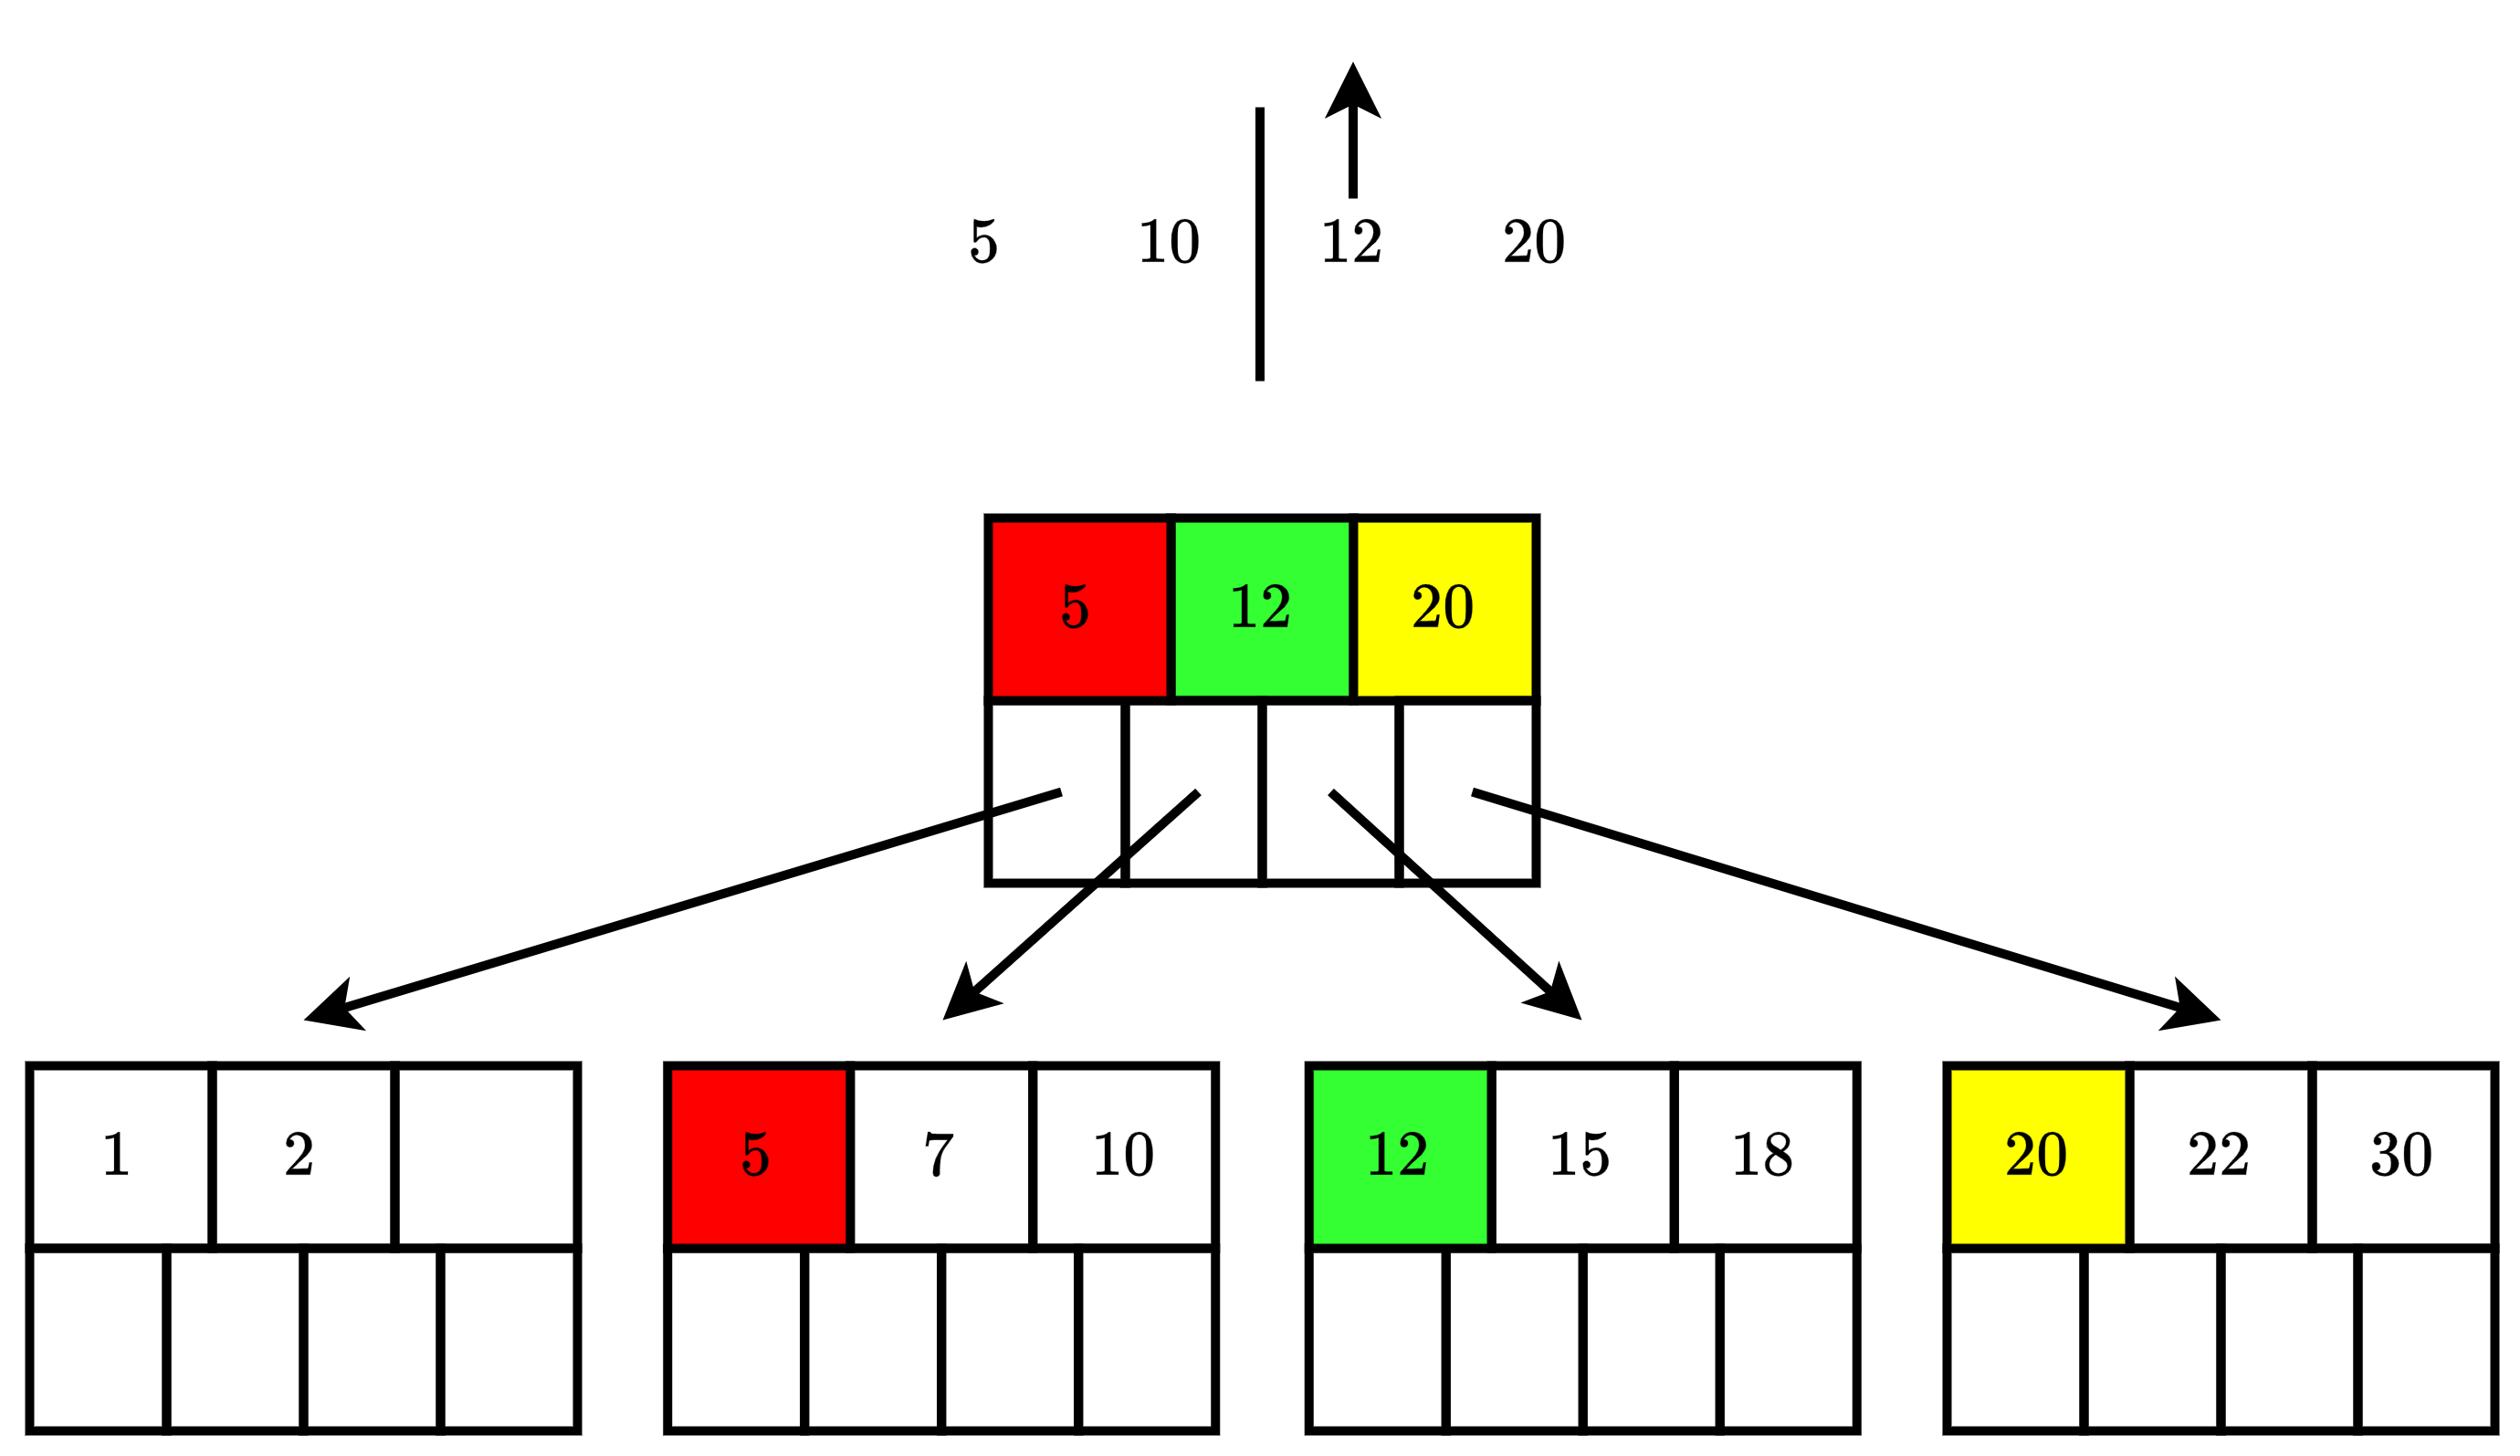
\includegraphics[width=0.7\textwidth]{diagram/P3-1-12-2.png}
                    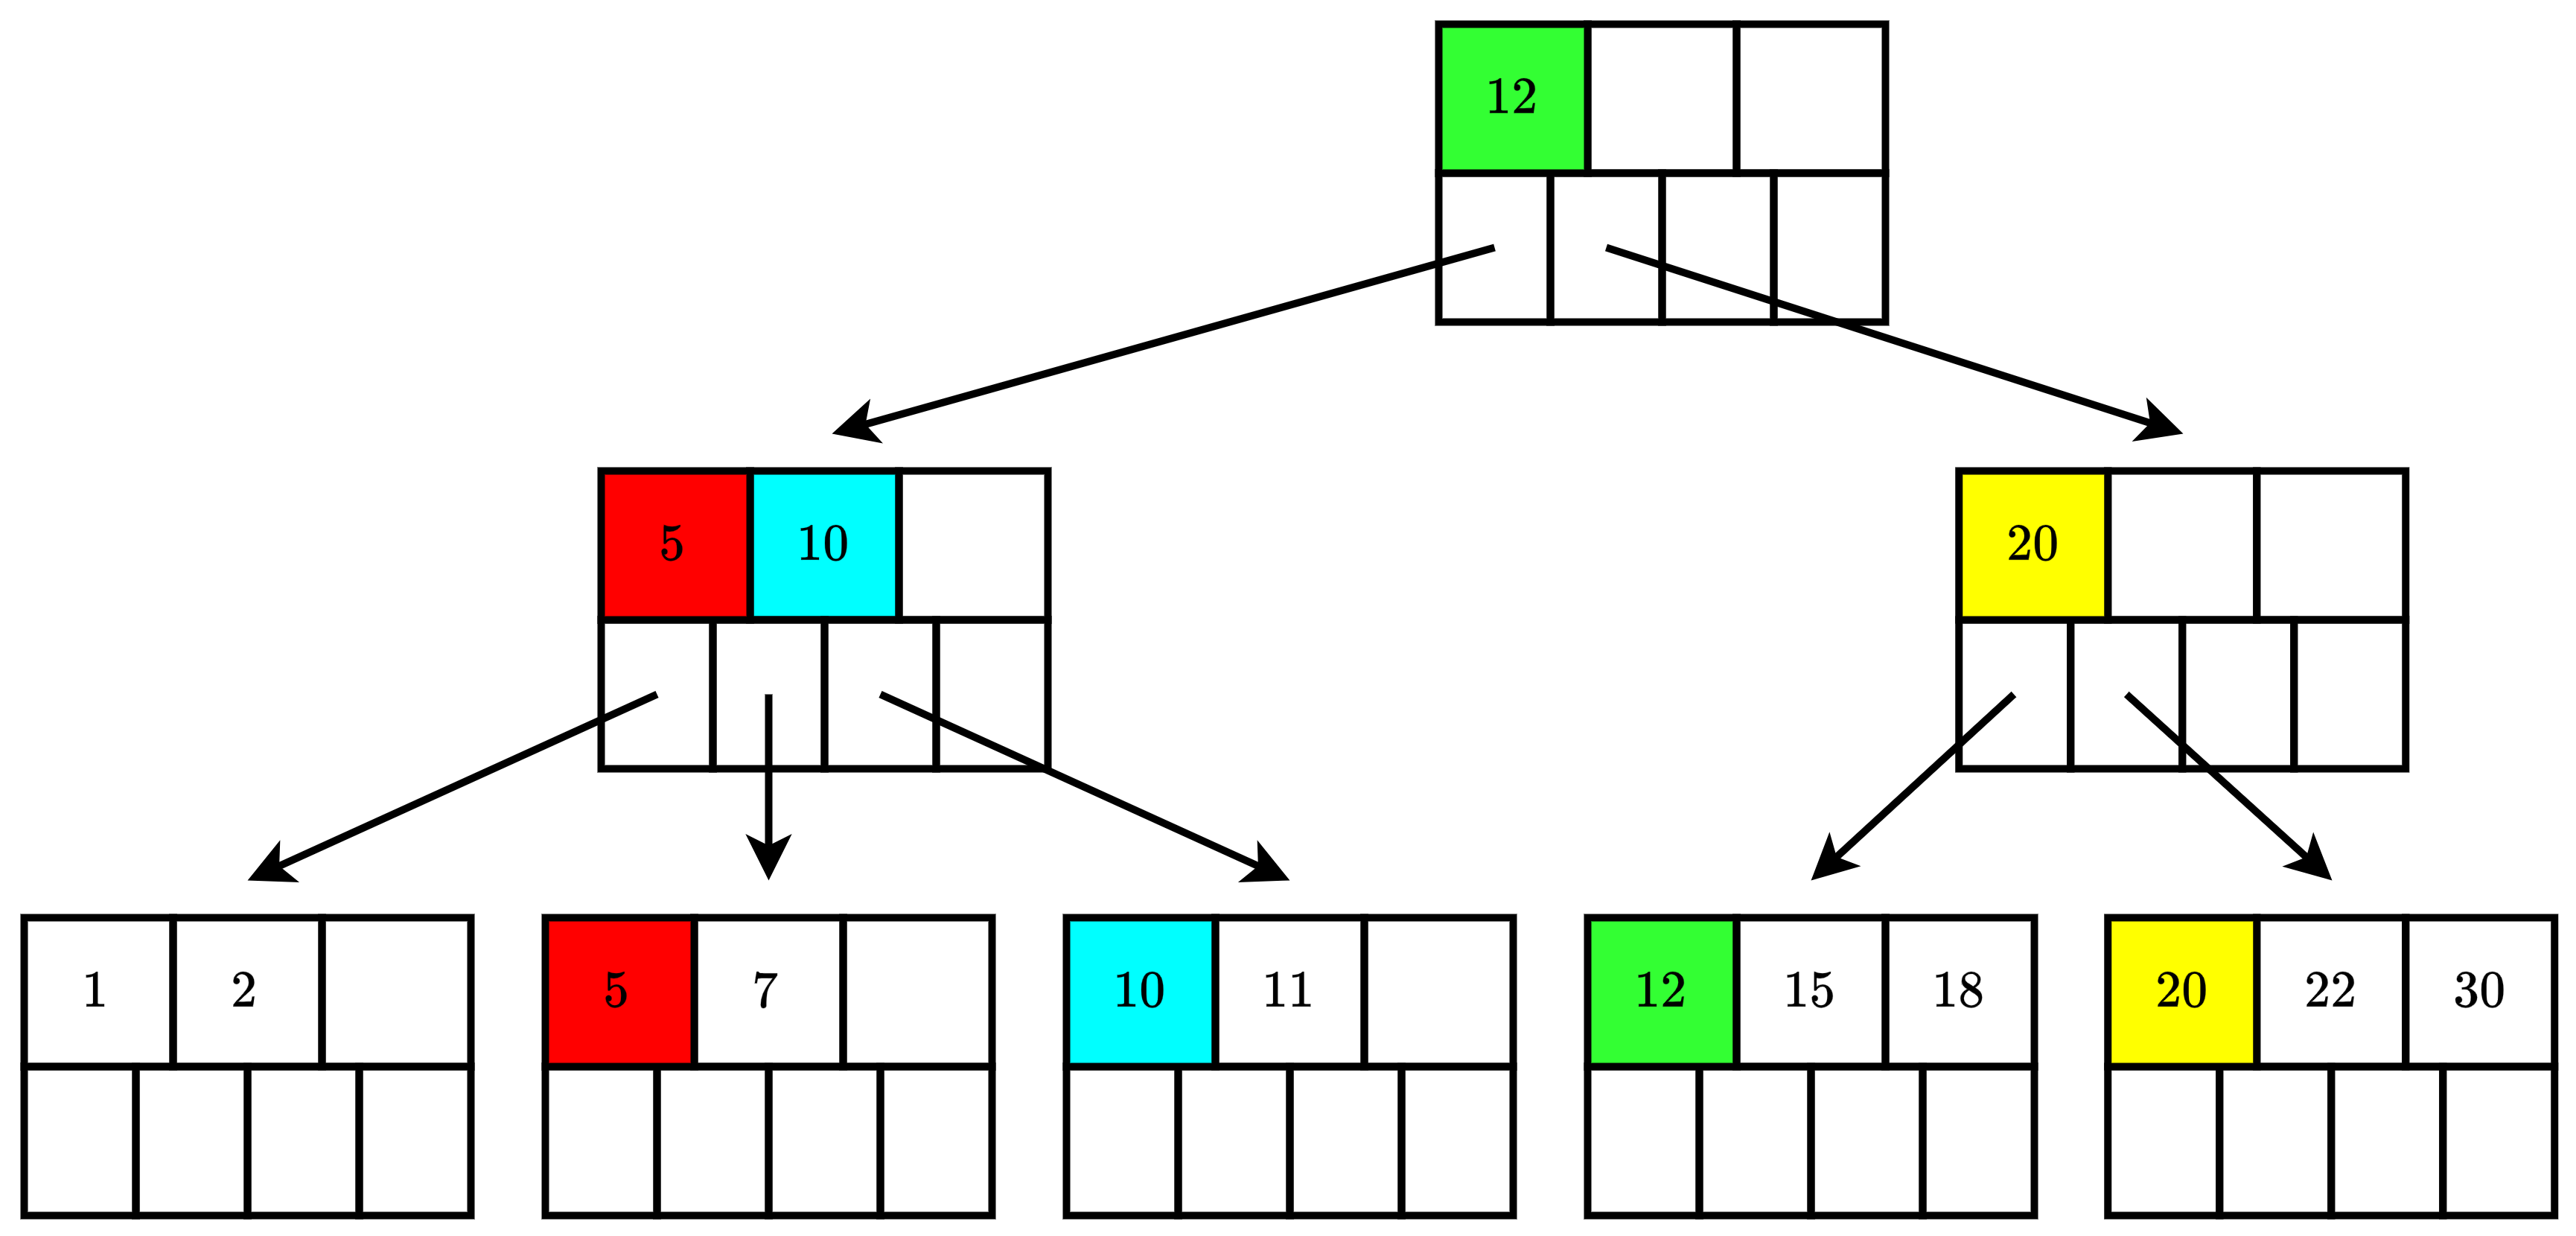
\includegraphics[width=0.8\textwidth]{diagram/P3-1-12-3.png}
                \end{figure}

                \newpage
                \item Ingresa 31:
                \begin{figure}[H]
                    \centering
                    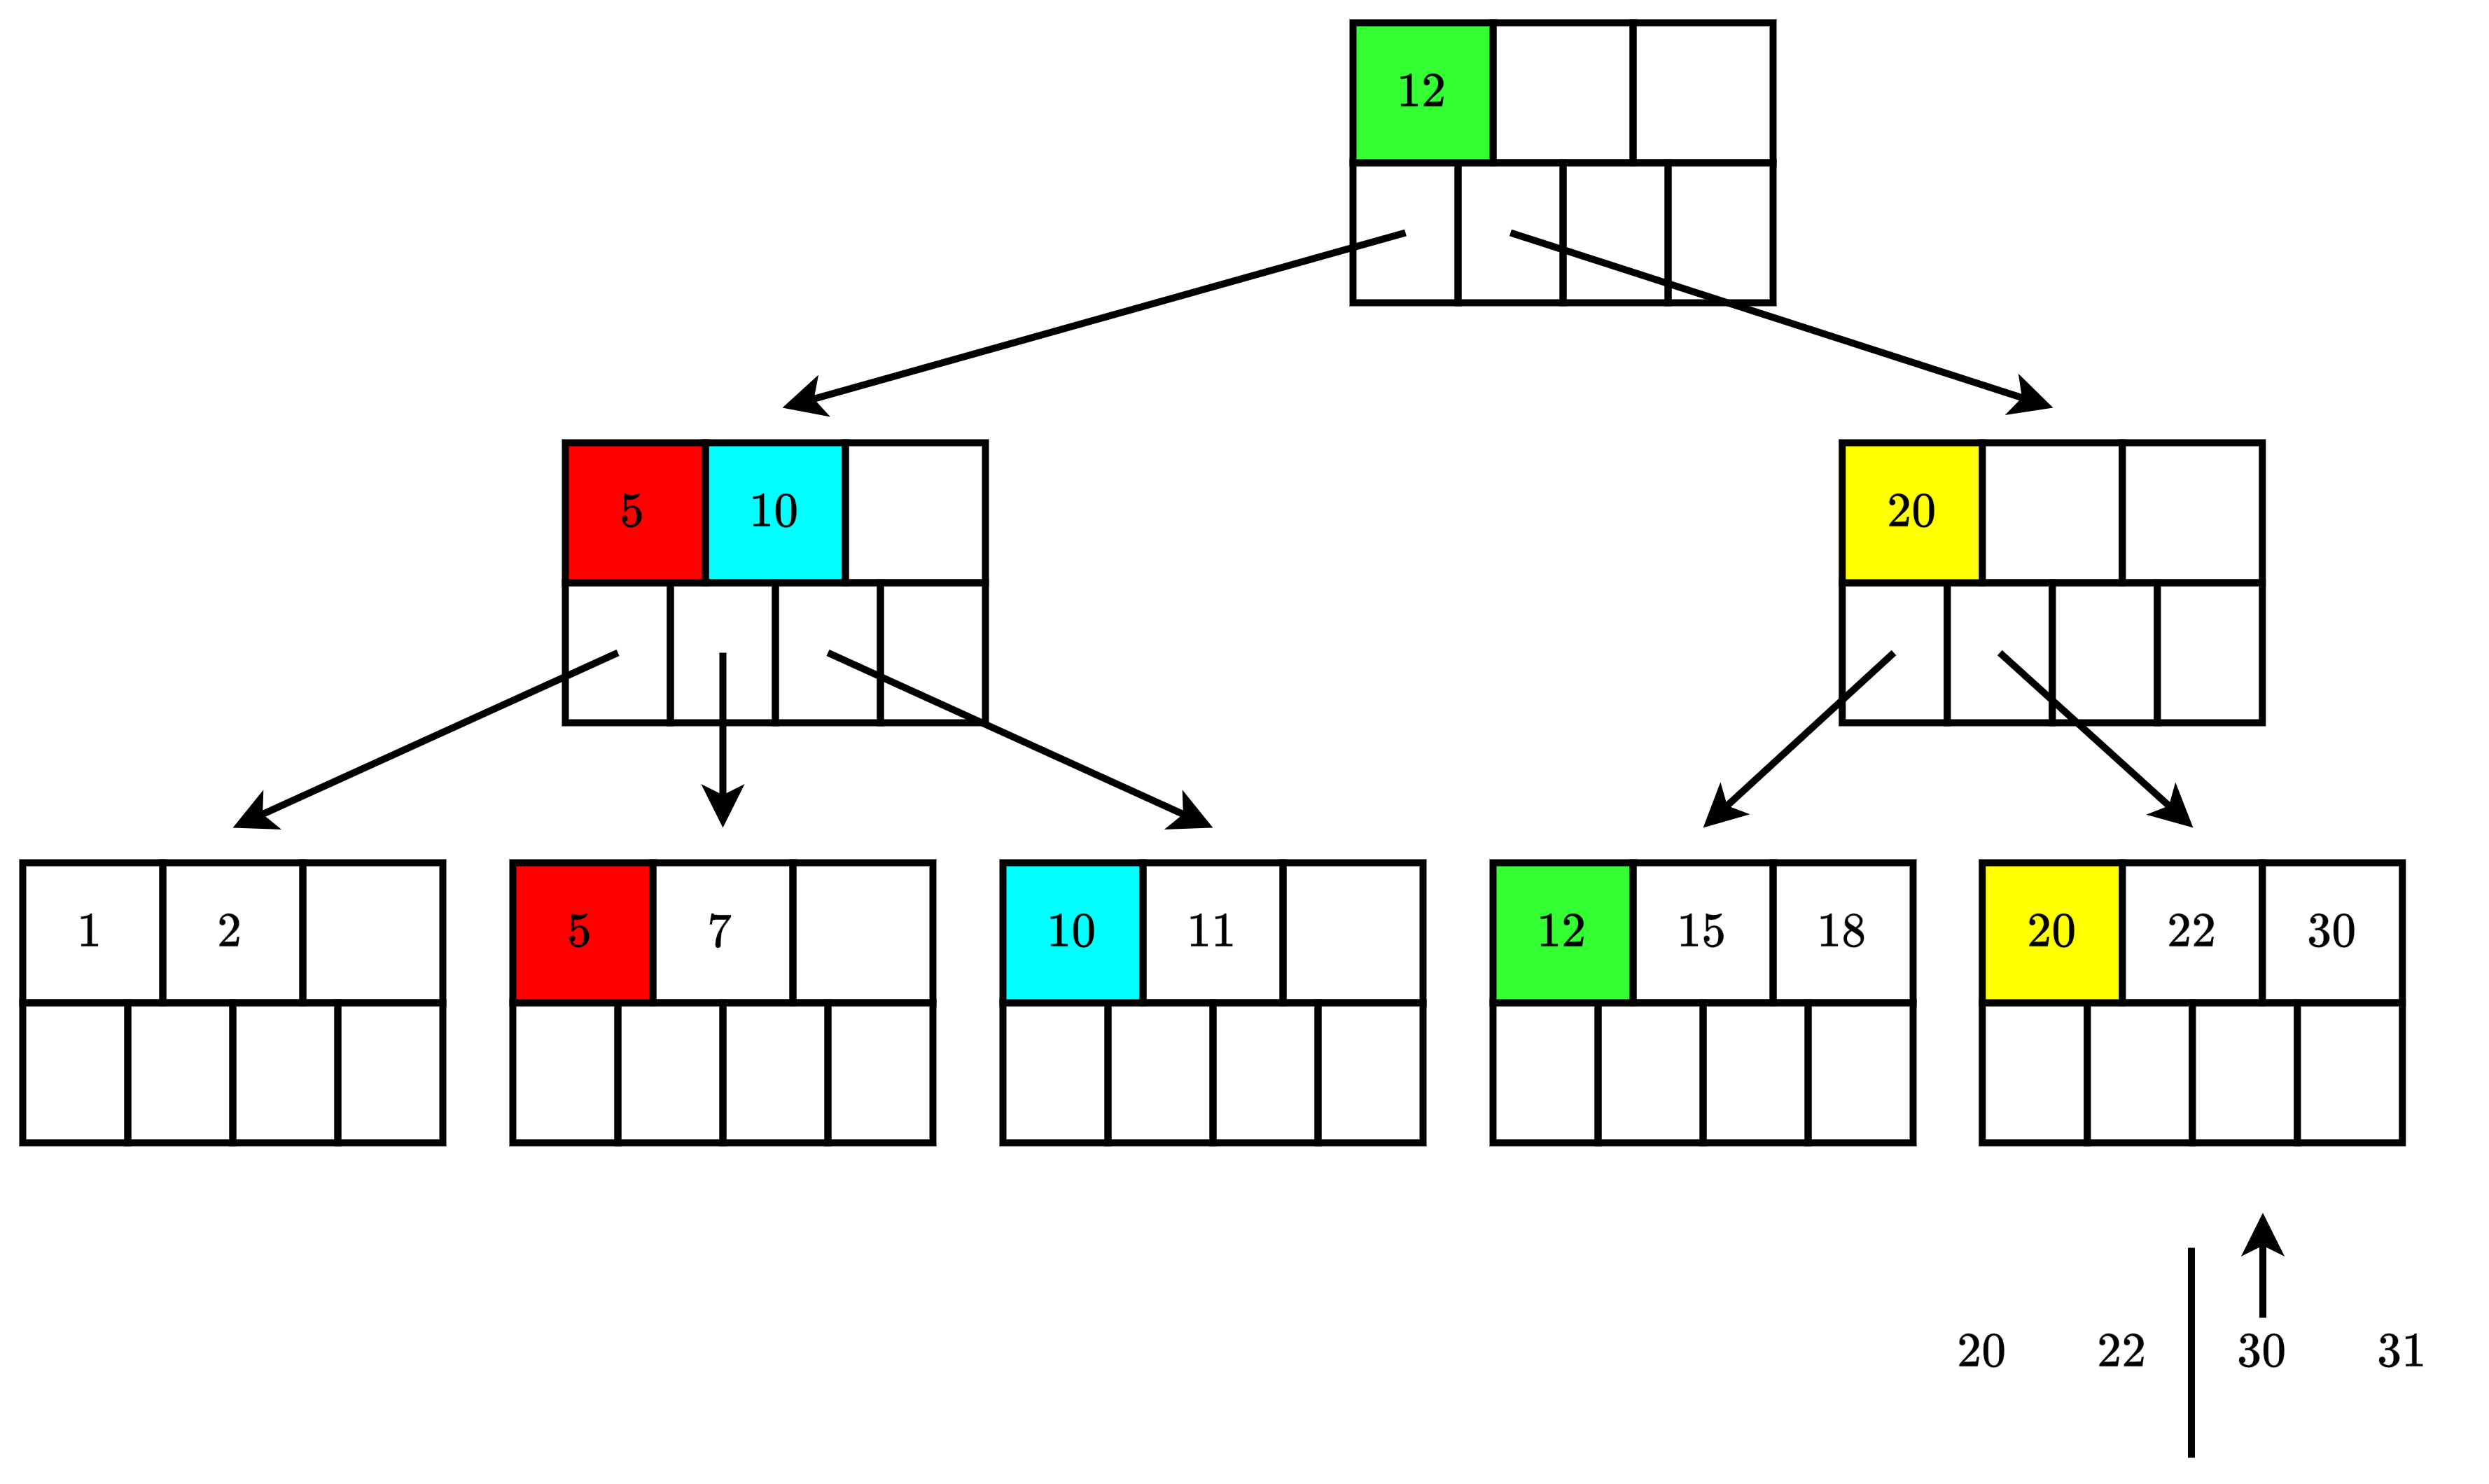
\includegraphics[width=0.85\textwidth]{diagram/P3-1-13-1.png}
                    \rule{\textwidth}{1pt}
                    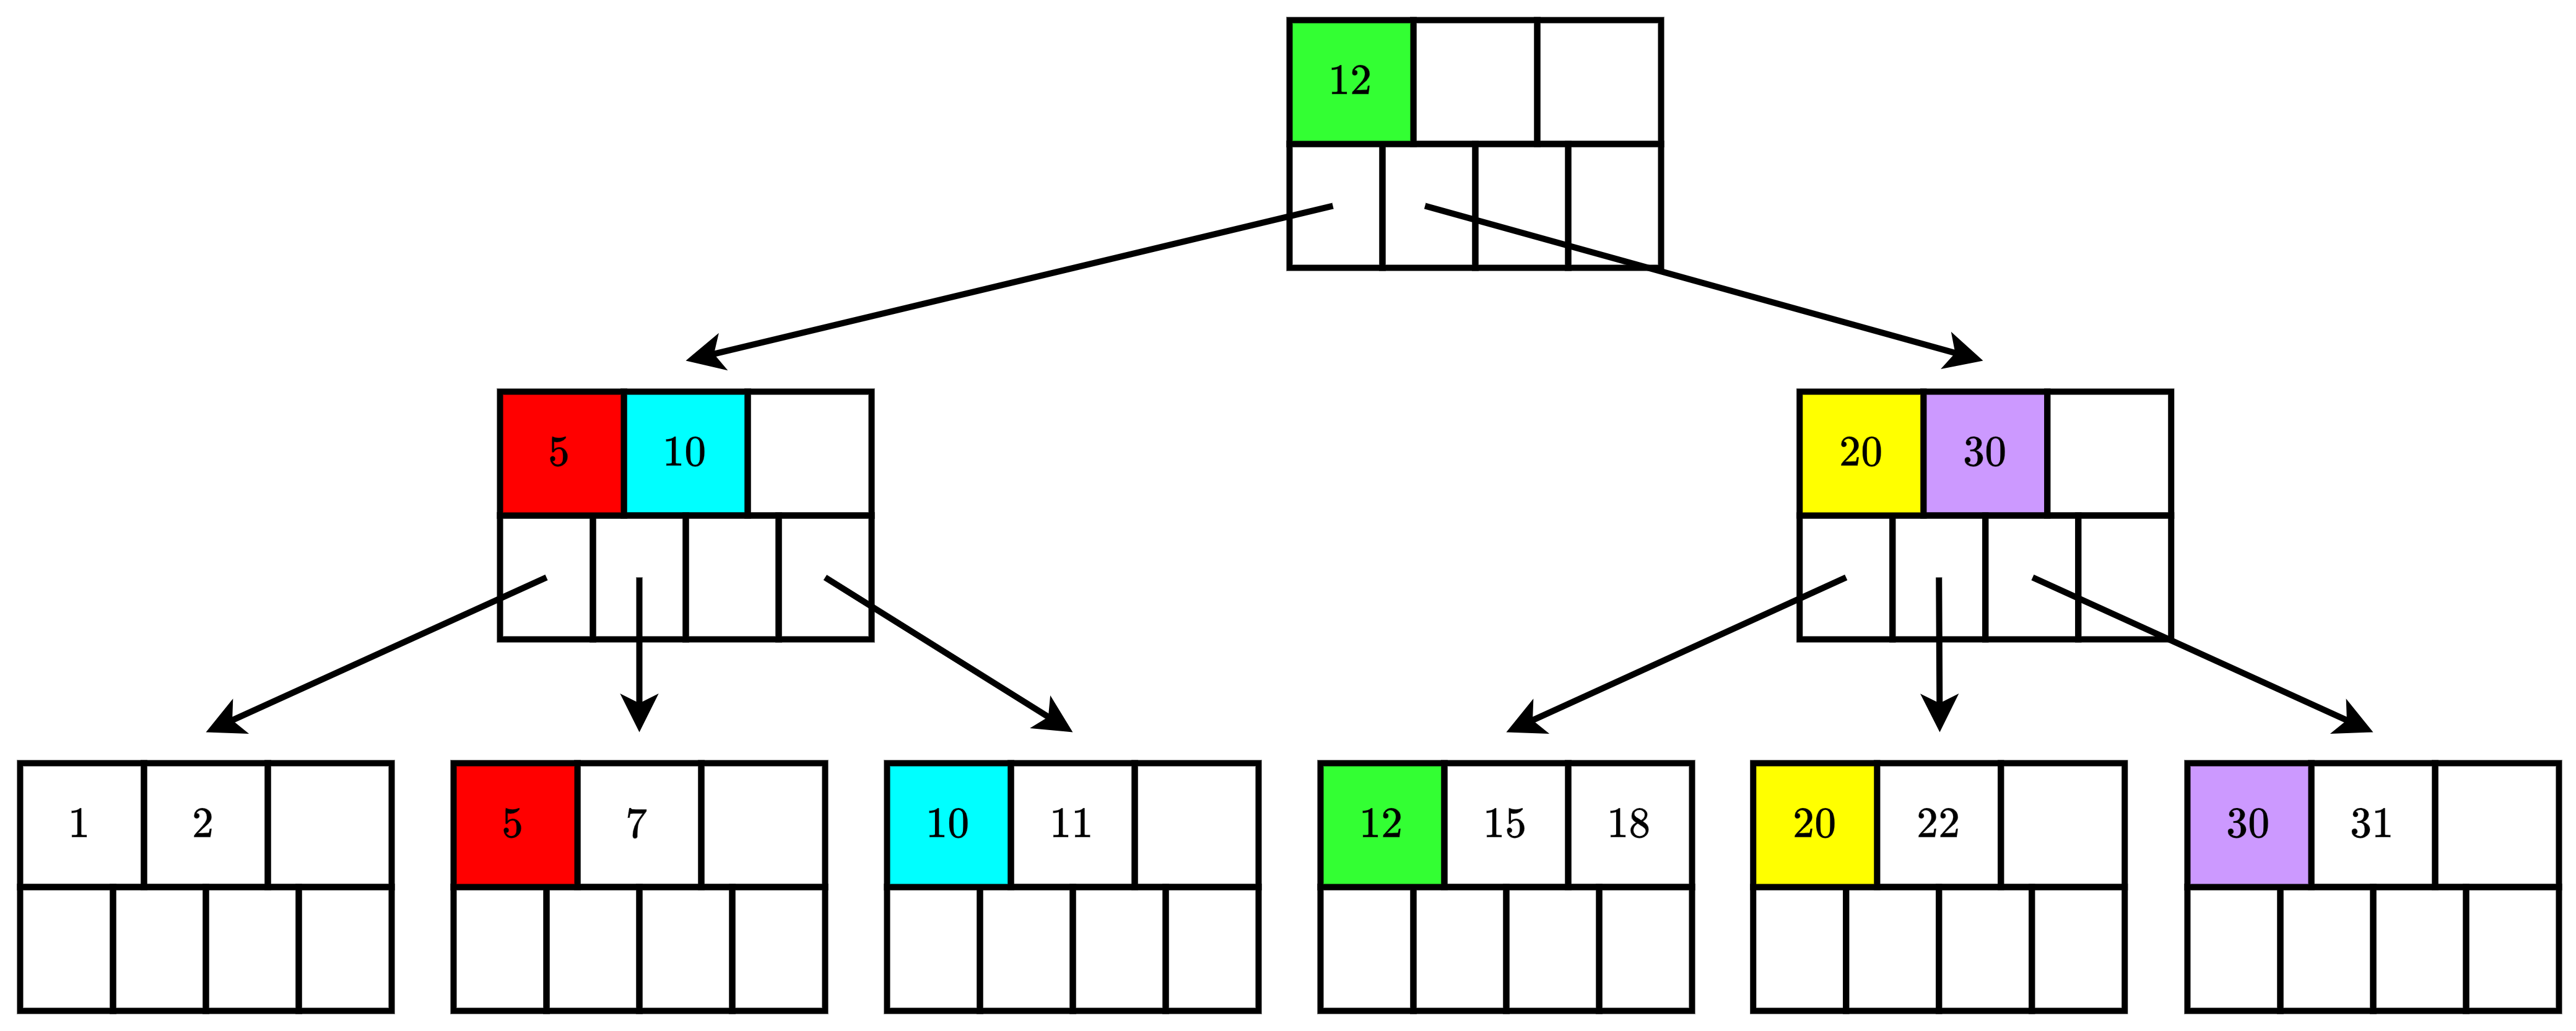
\includegraphics[width=0.8\textwidth]{diagram/P3-1-13-2.png}
                \end{figure}

                \item Ingresa 40:
                \begin{figure}[H]
                    \centering
                    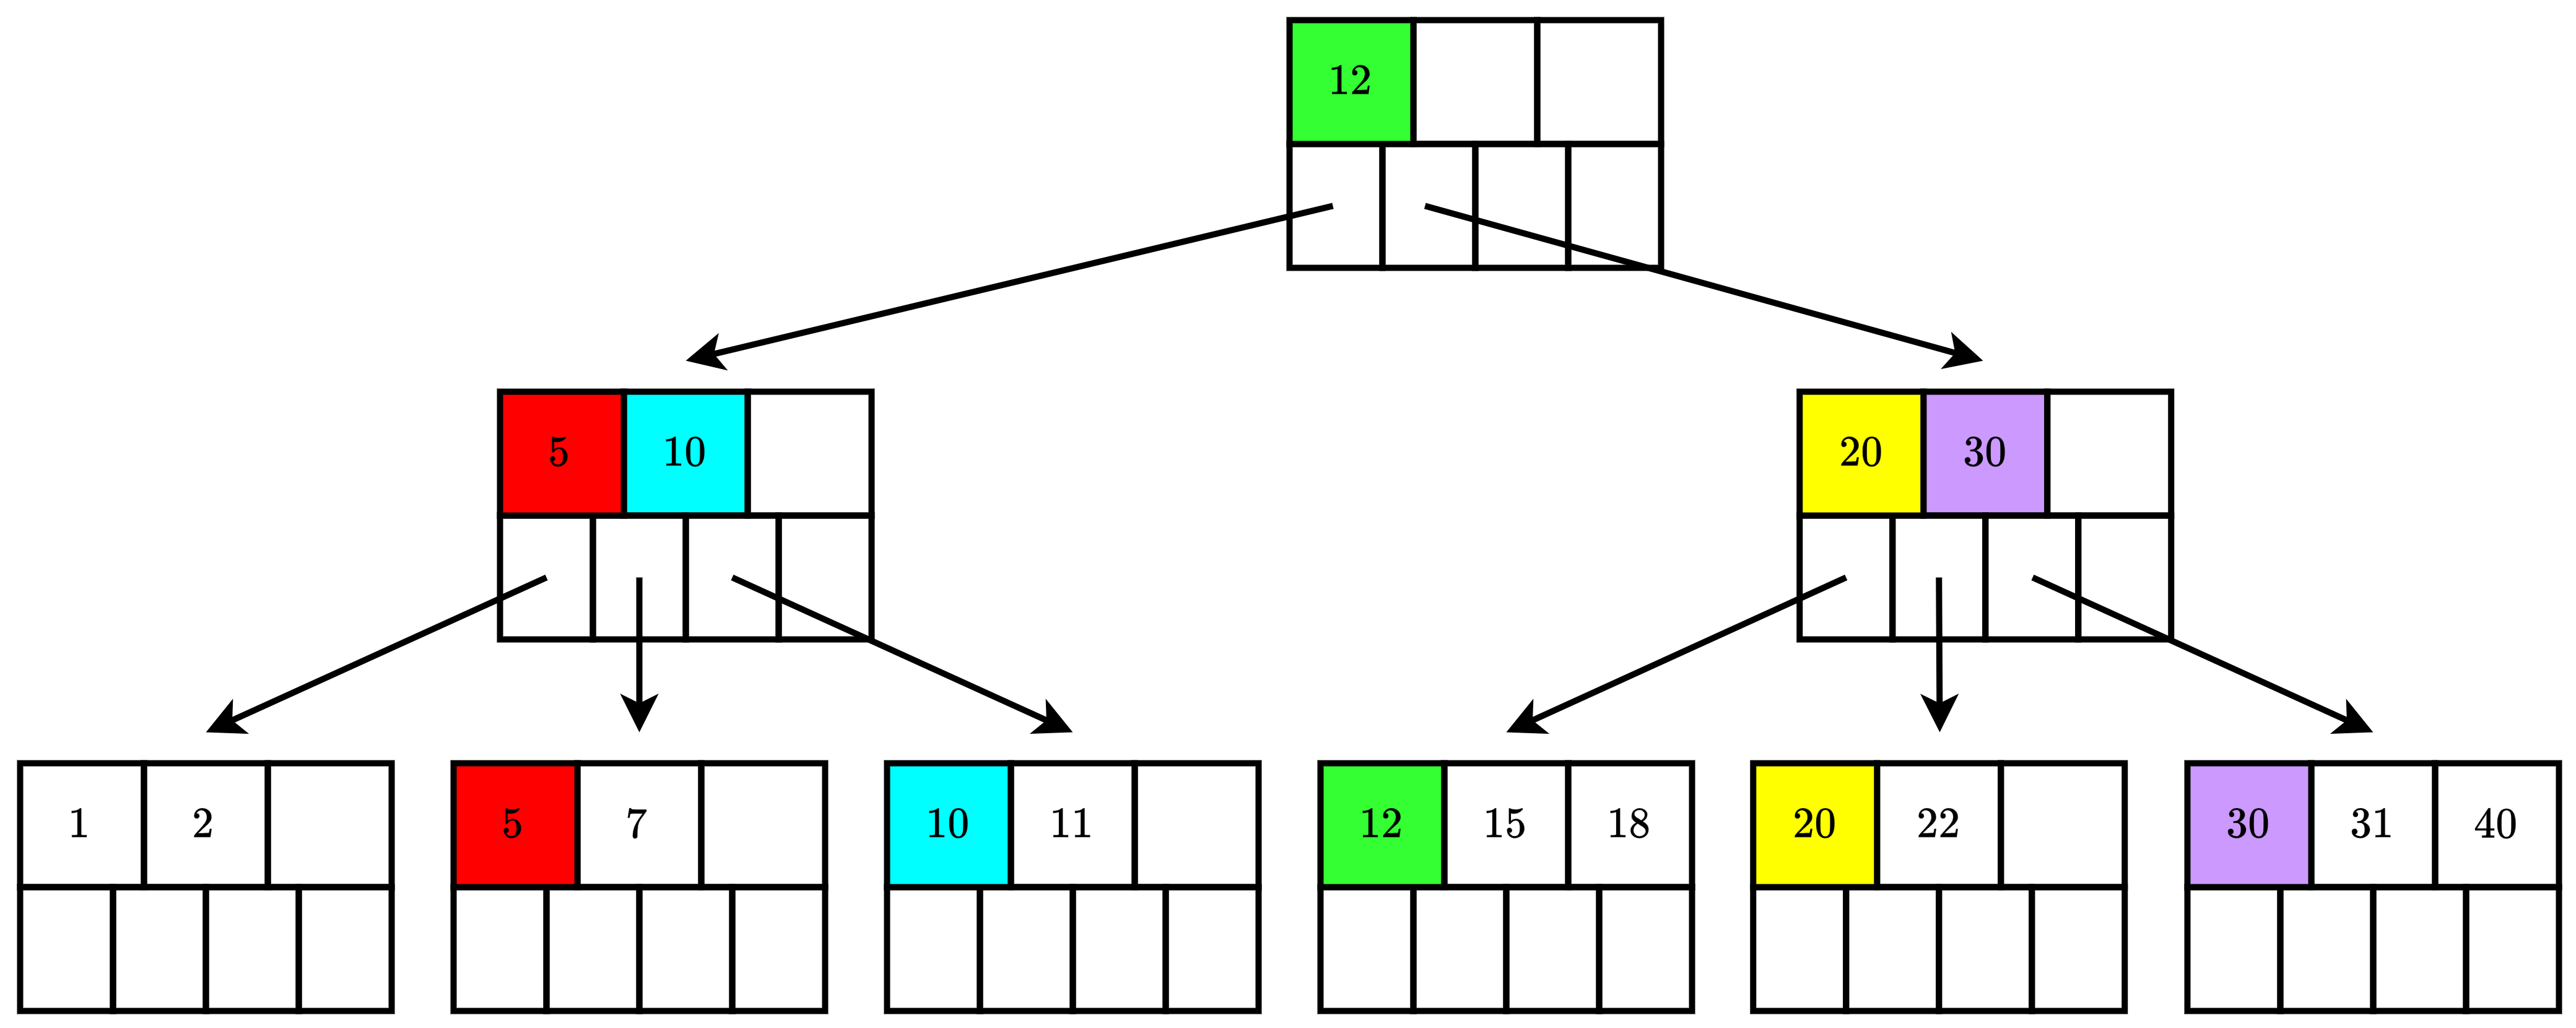
\includegraphics[width=0.8\textwidth]{diagram/P3-1-14.png}
                \end{figure}

                \newpage
                \item Ingresa 50:
                \begin{figure}[H]
                    \centering
                    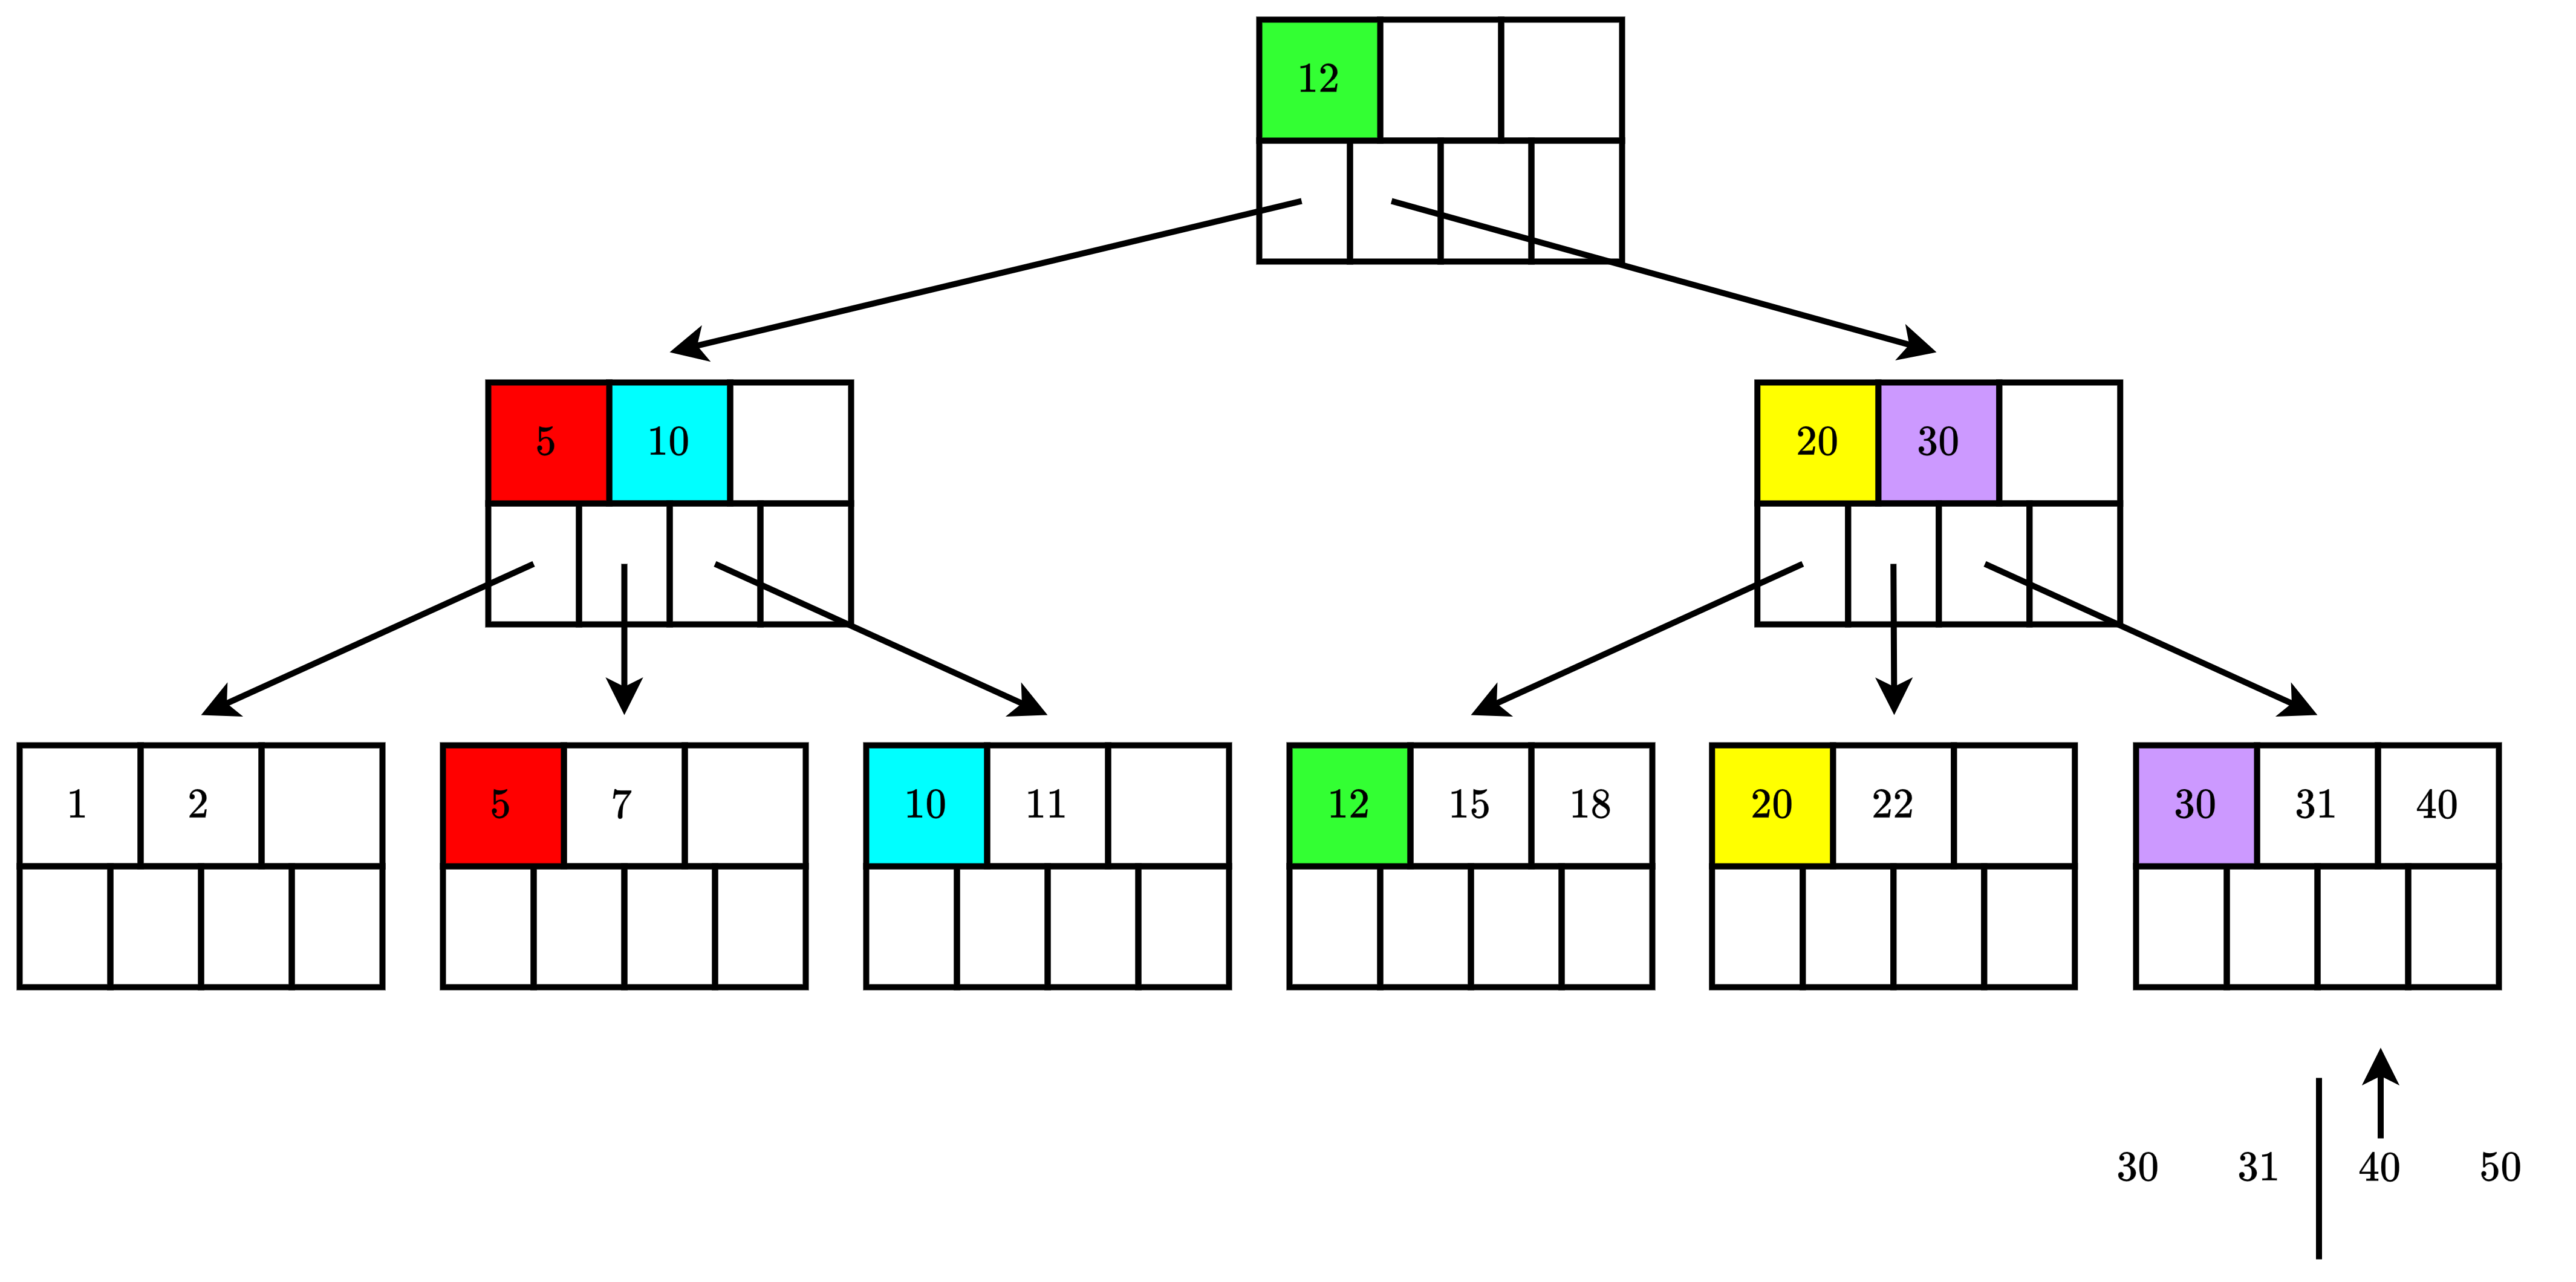
\includegraphics[width=0.8\textwidth]{diagram/P3-1-15-1.png}
                    \rule{\textwidth}{1pt}
                    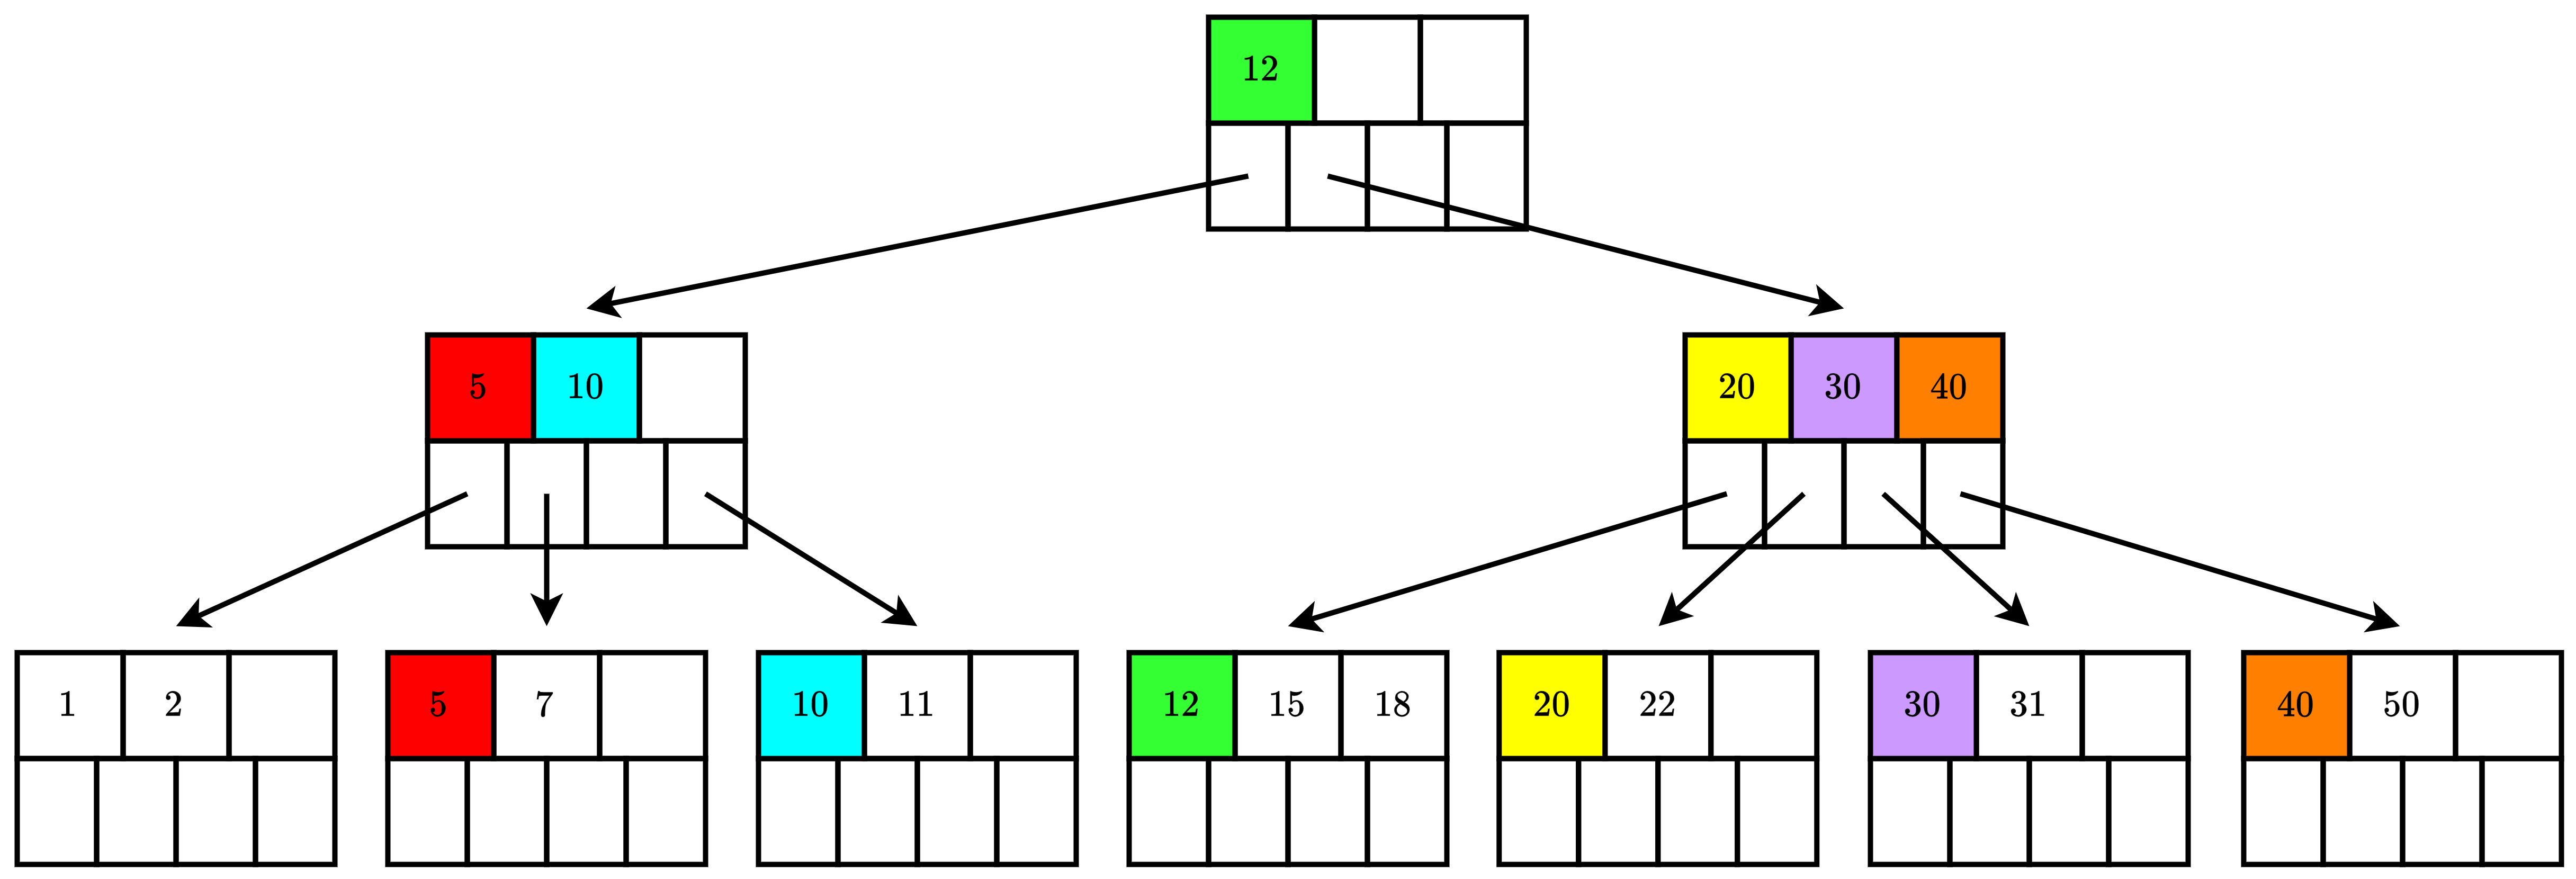
\includegraphics[width=0.8\textwidth]{diagram/P3-1-15-2.png}
                \end{figure}

                \item Ingresa 35:
                \begin{figure}[H]
                    \centering
                    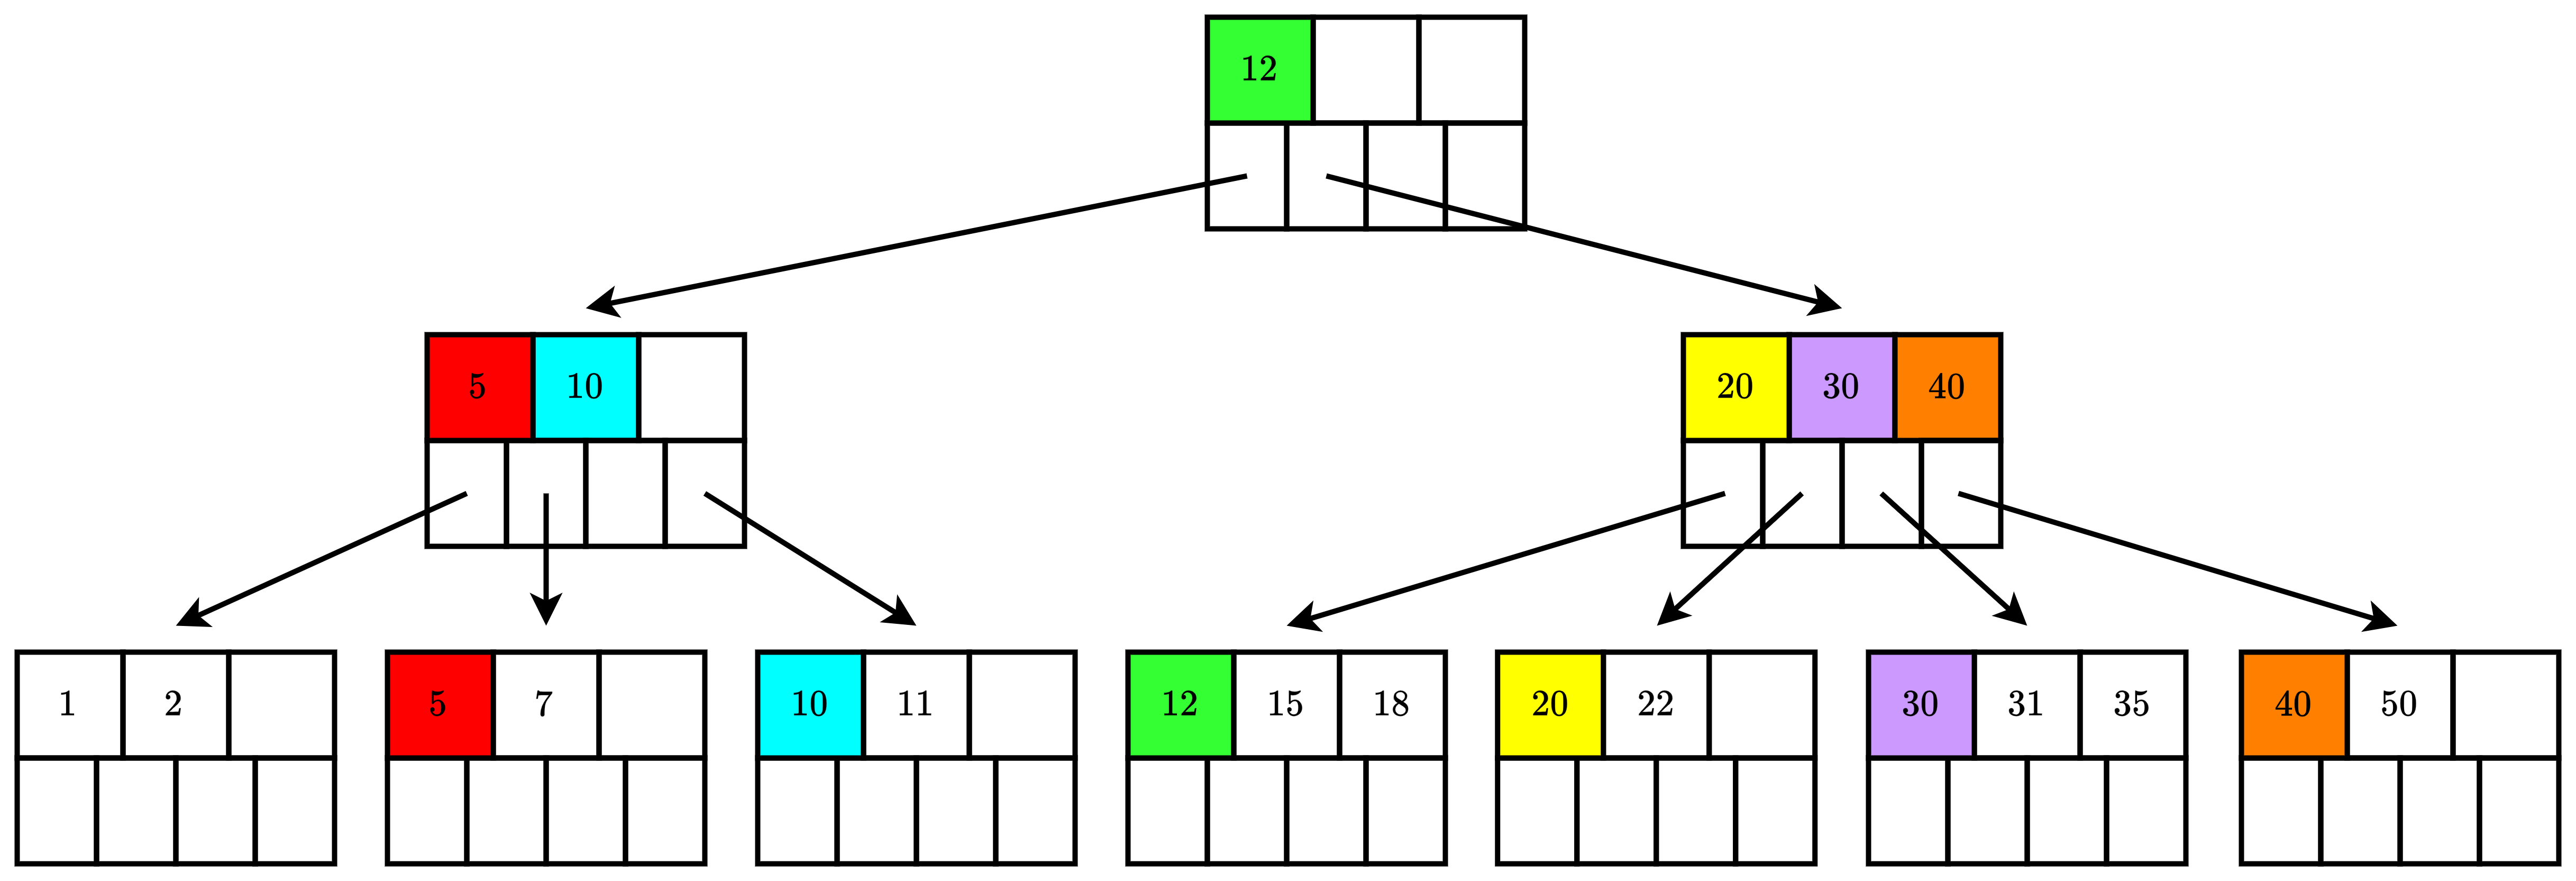
\includegraphics[width=0.8\textwidth]{diagram/P3-1-16.png}
                \end{figure}

                \newpage
                \item Ingresa 37:
                \begin{figure}[H]
                    \centering
                    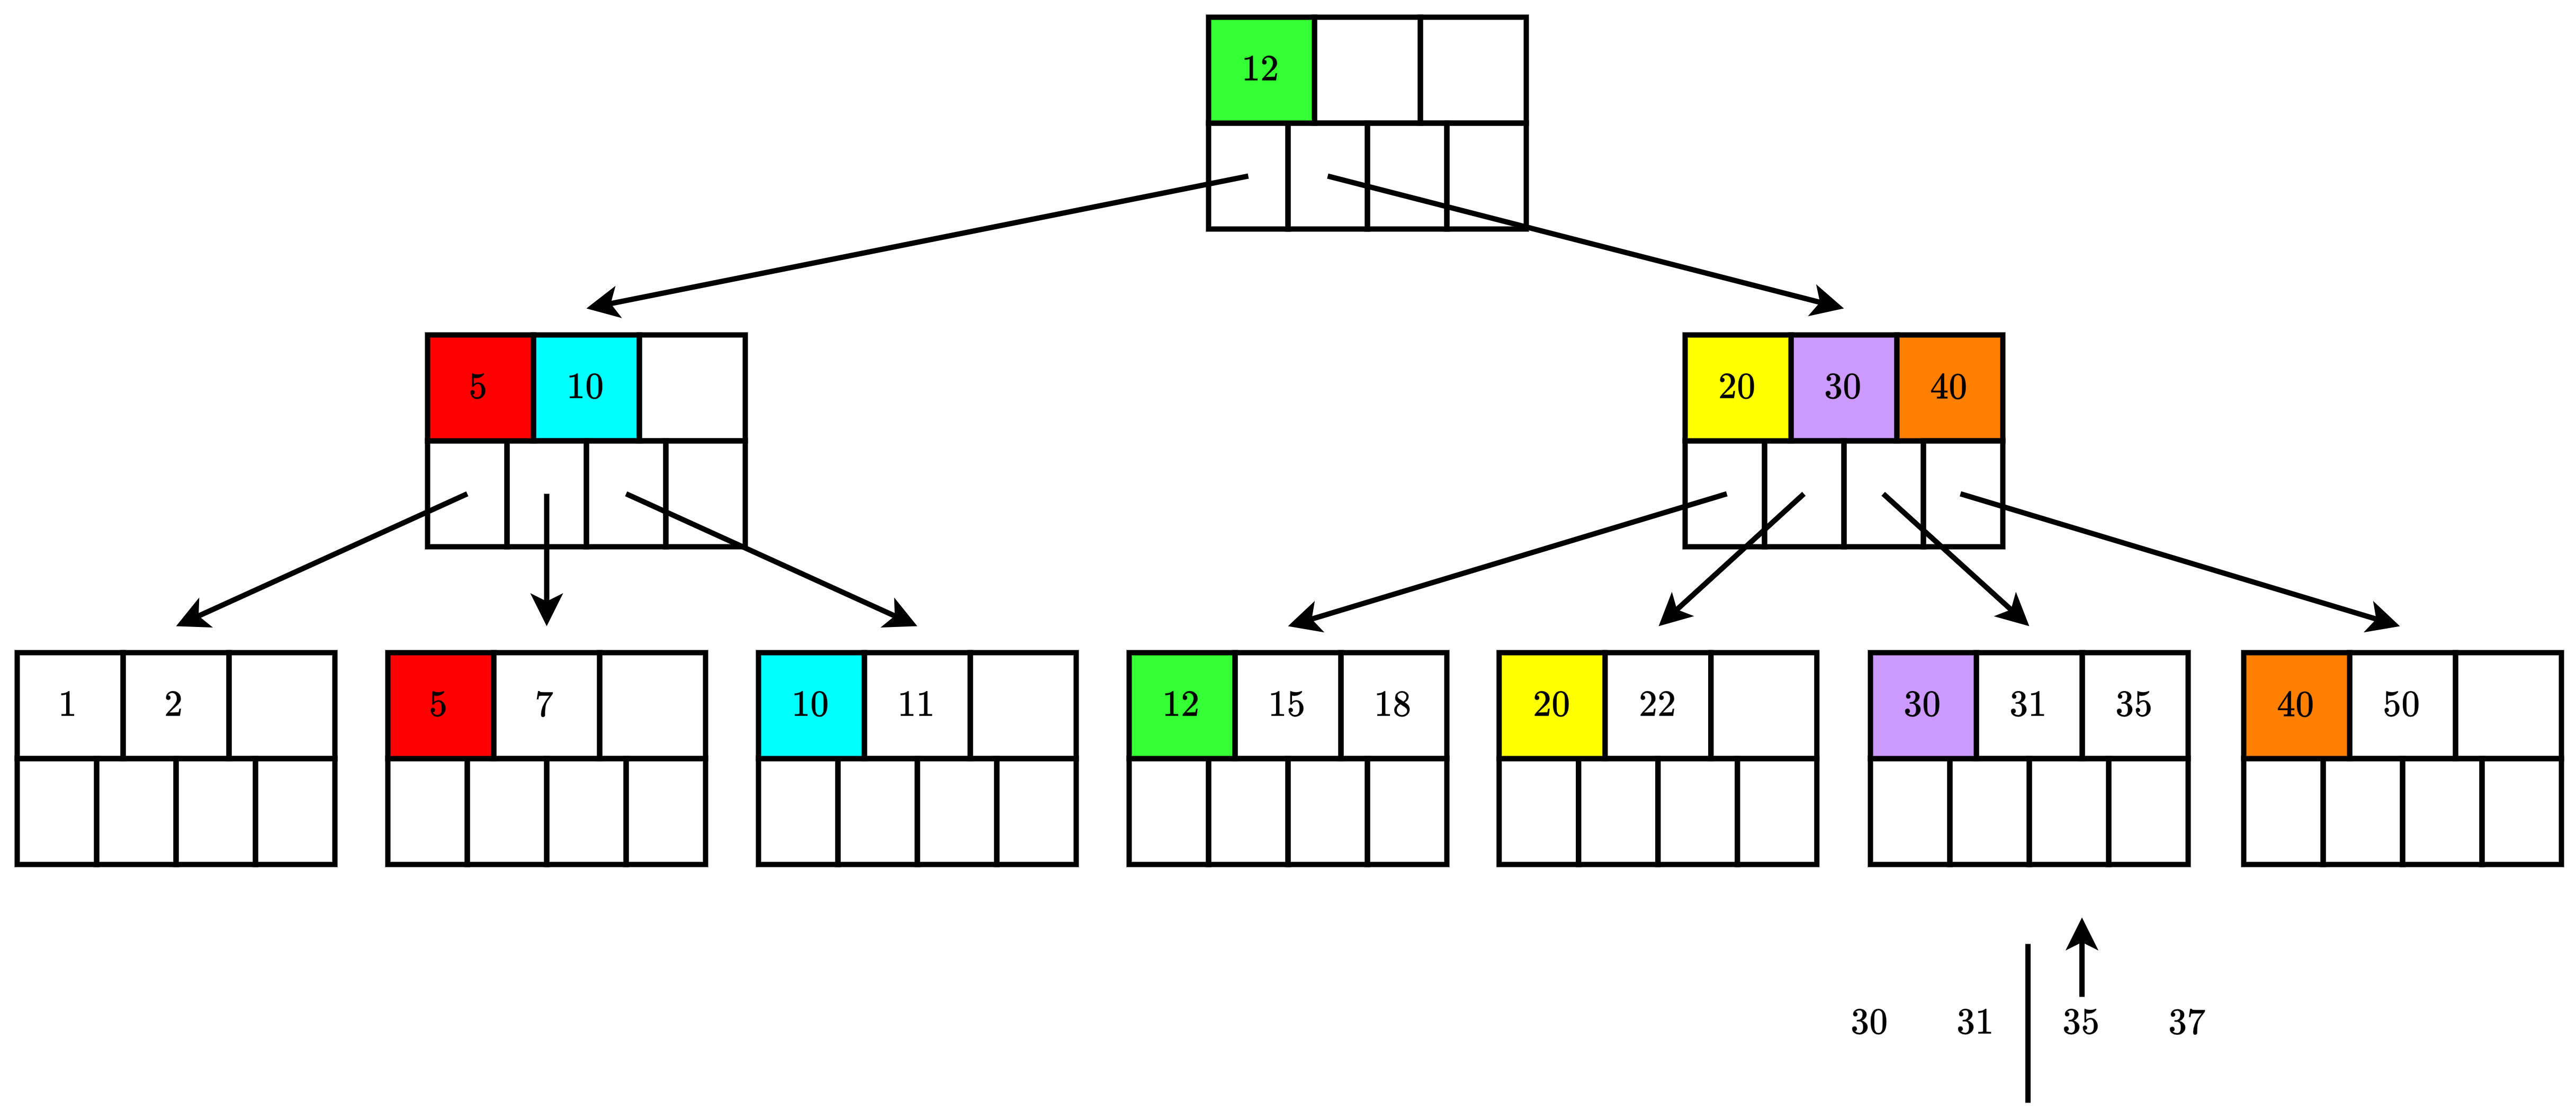
\includegraphics[width=0.6\textwidth]{diagram/P3-1-17-1.png}
                    \rule{\textwidth}{1pt}
                    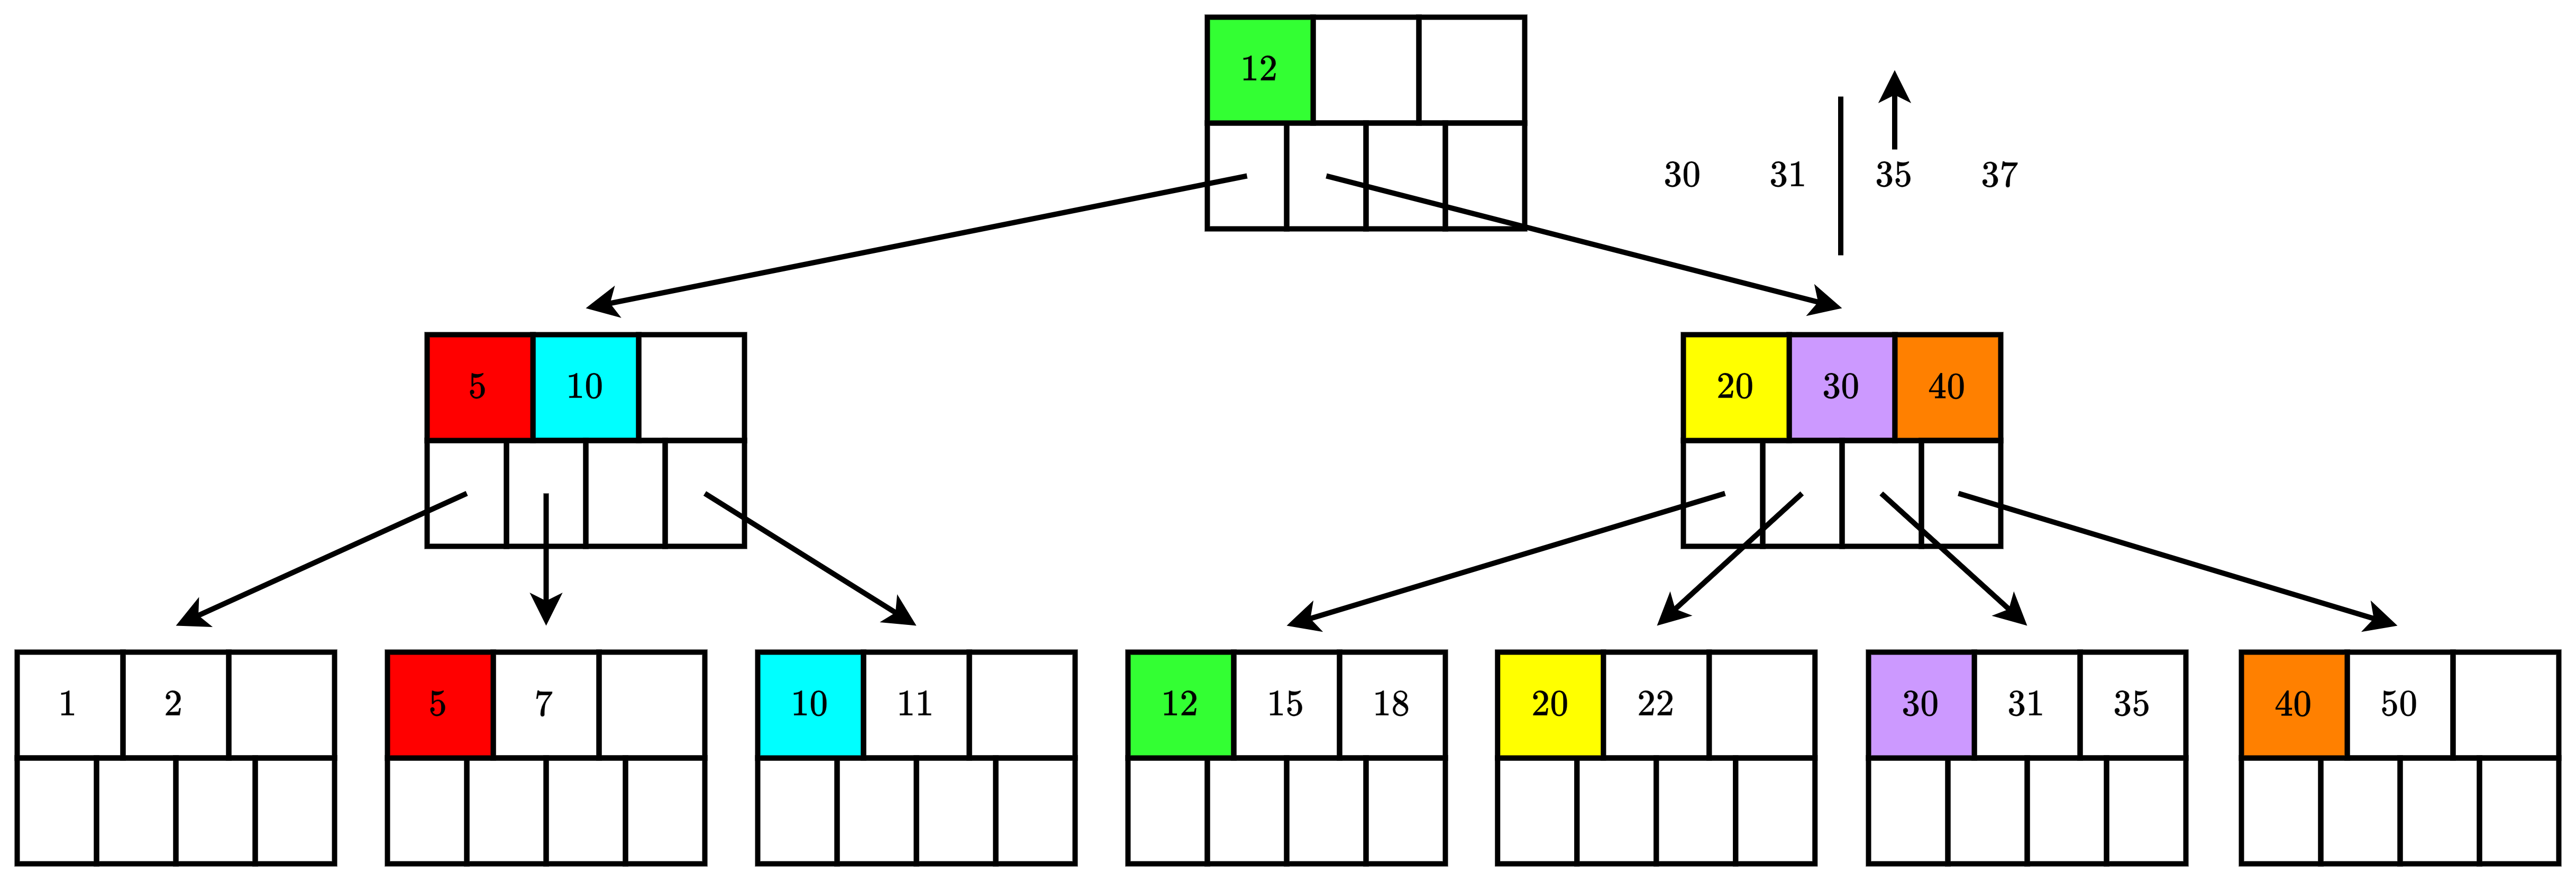
\includegraphics[width=0.7\textwidth]{diagram/P3-1-17-2.png}
                    \rule{\textwidth}{1pt}
                    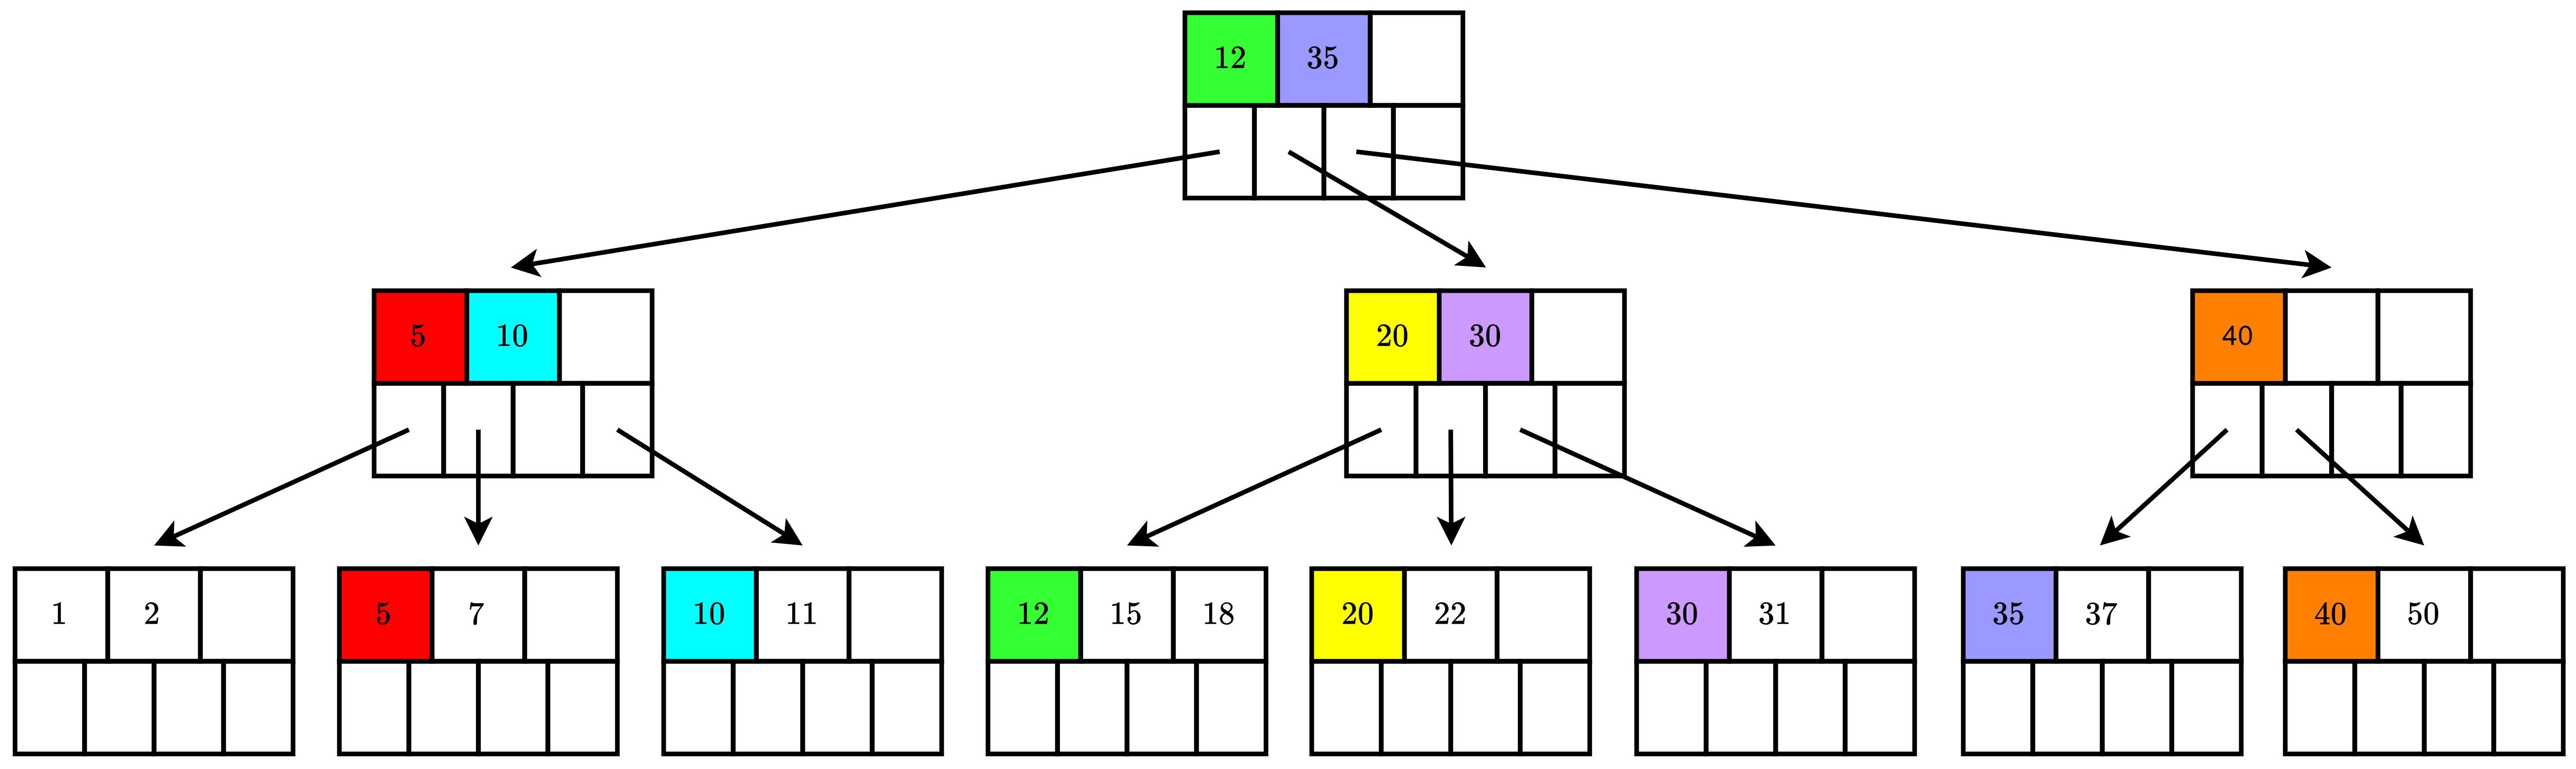
\includegraphics[width=0.8\textwidth]{diagram/P3-1-17-3.png}
                \end{figure}

                \item Ingresa 21:
                \begin{figure}[H]
                    \centering
                    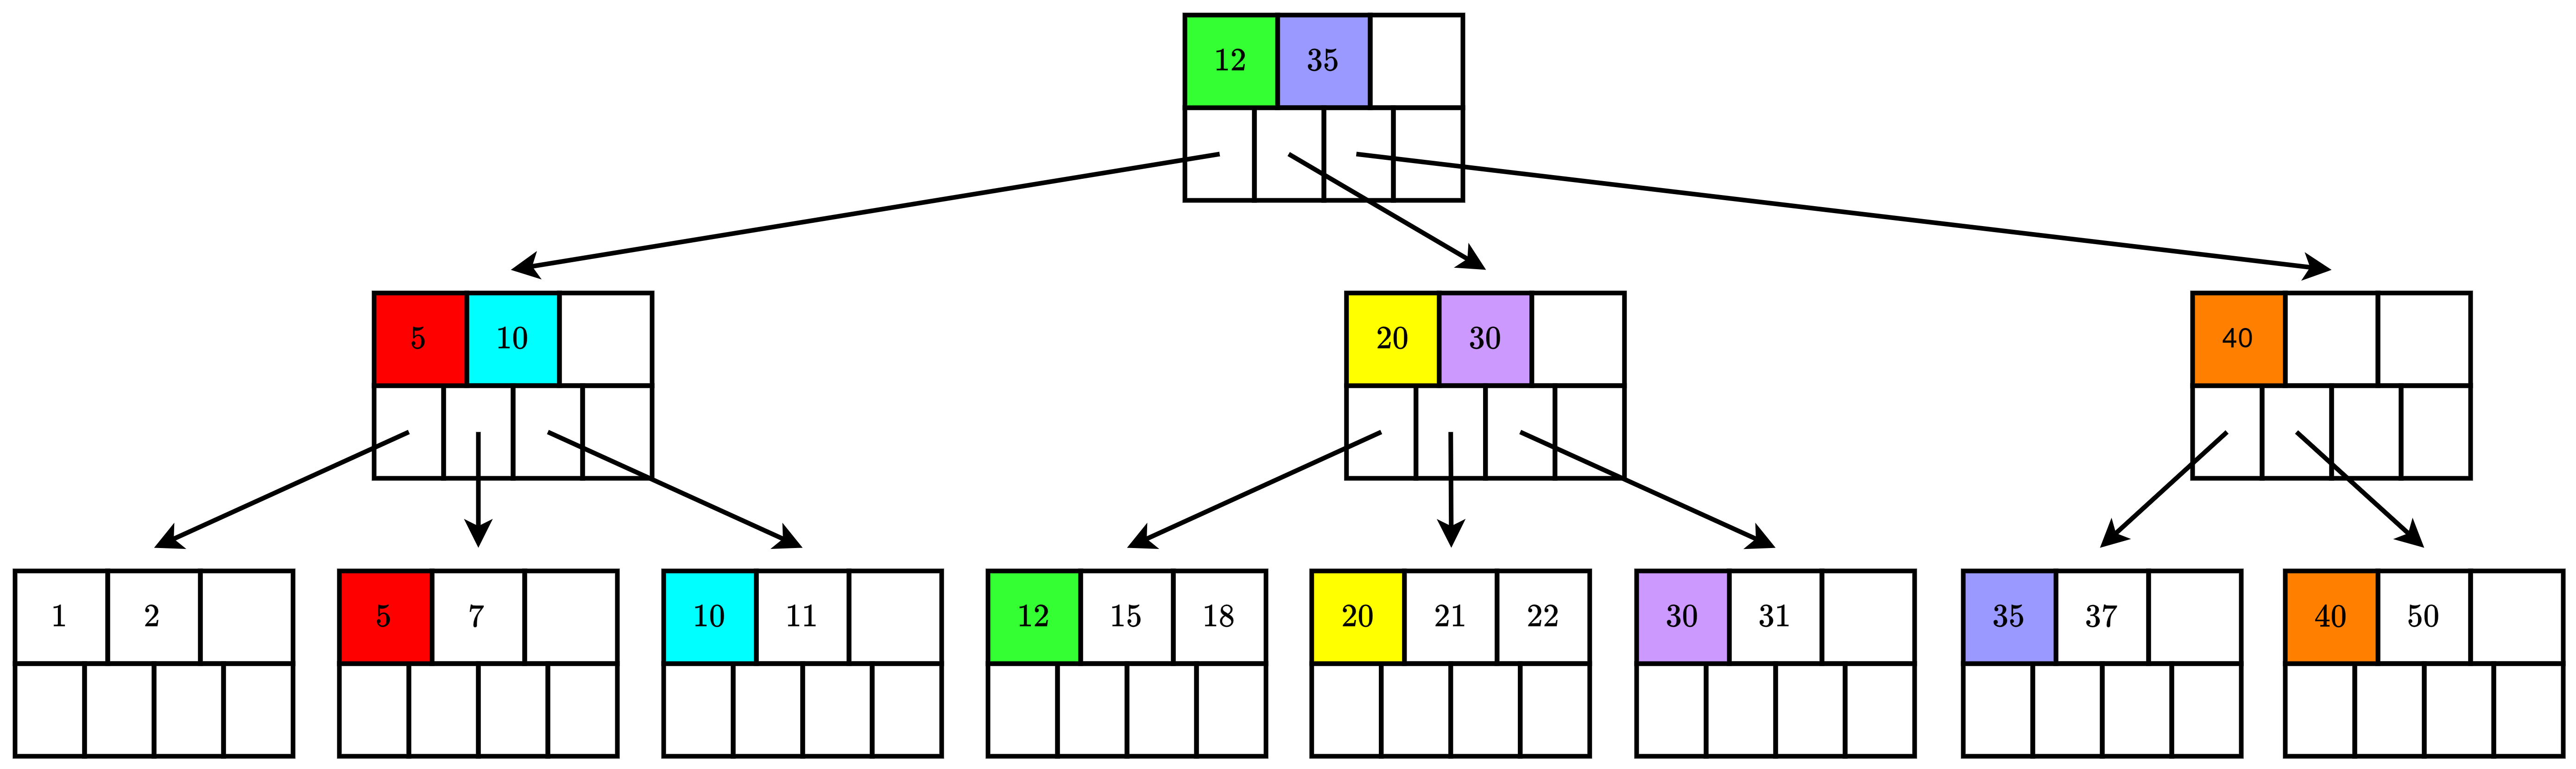
\includegraphics[width=0.8\textwidth]{diagram/P3-1-18.png}
                \end{figure}

                \newpage
                \item Ingresa 23:
                \begin{figure}[H]
                    \centering
                    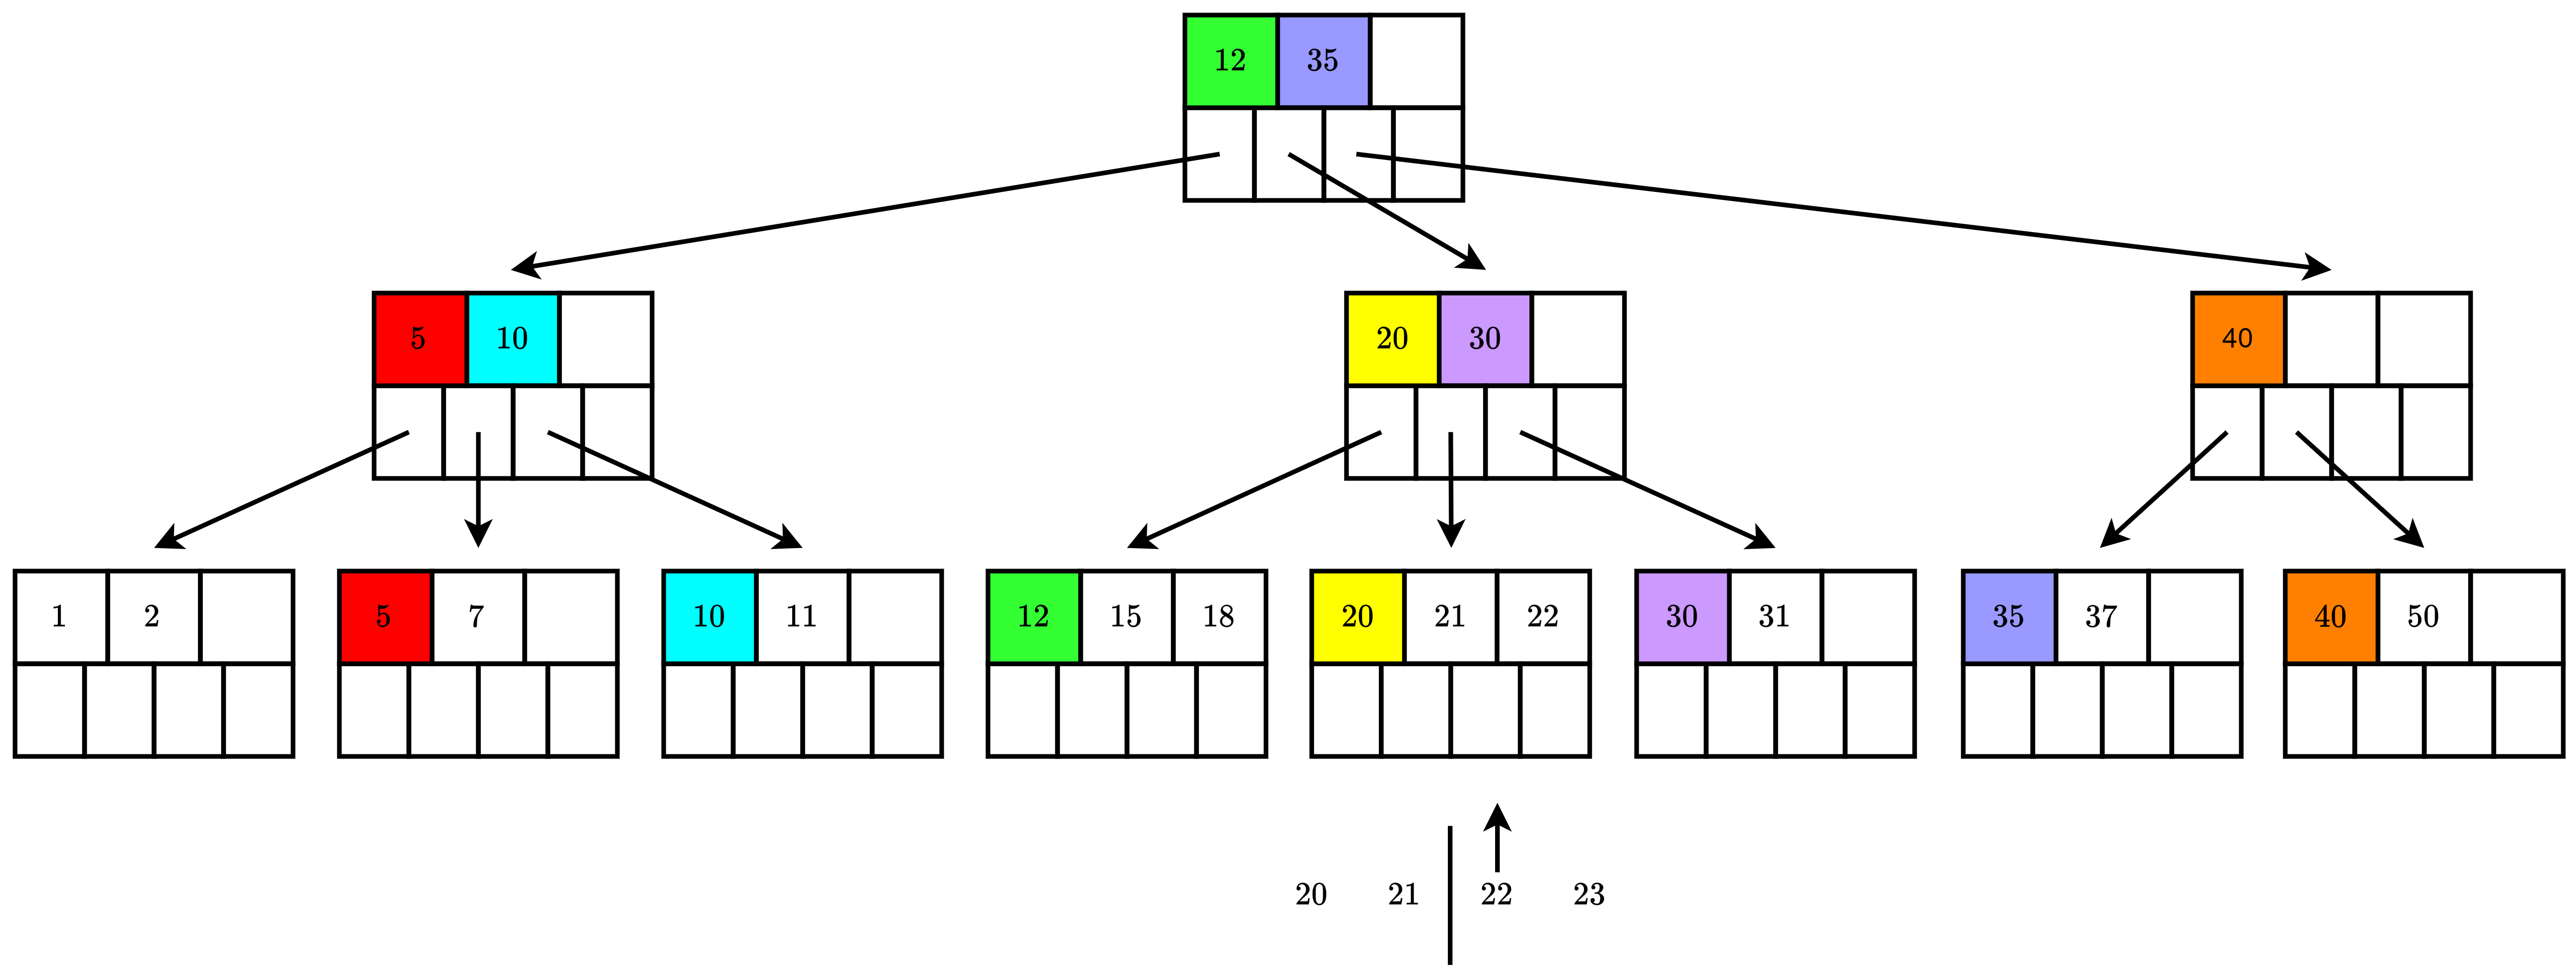
\includegraphics[width=0.8\textwidth]{diagram/P3-1-19-1.png}
                    \rule{\textwidth}{1pt}
                    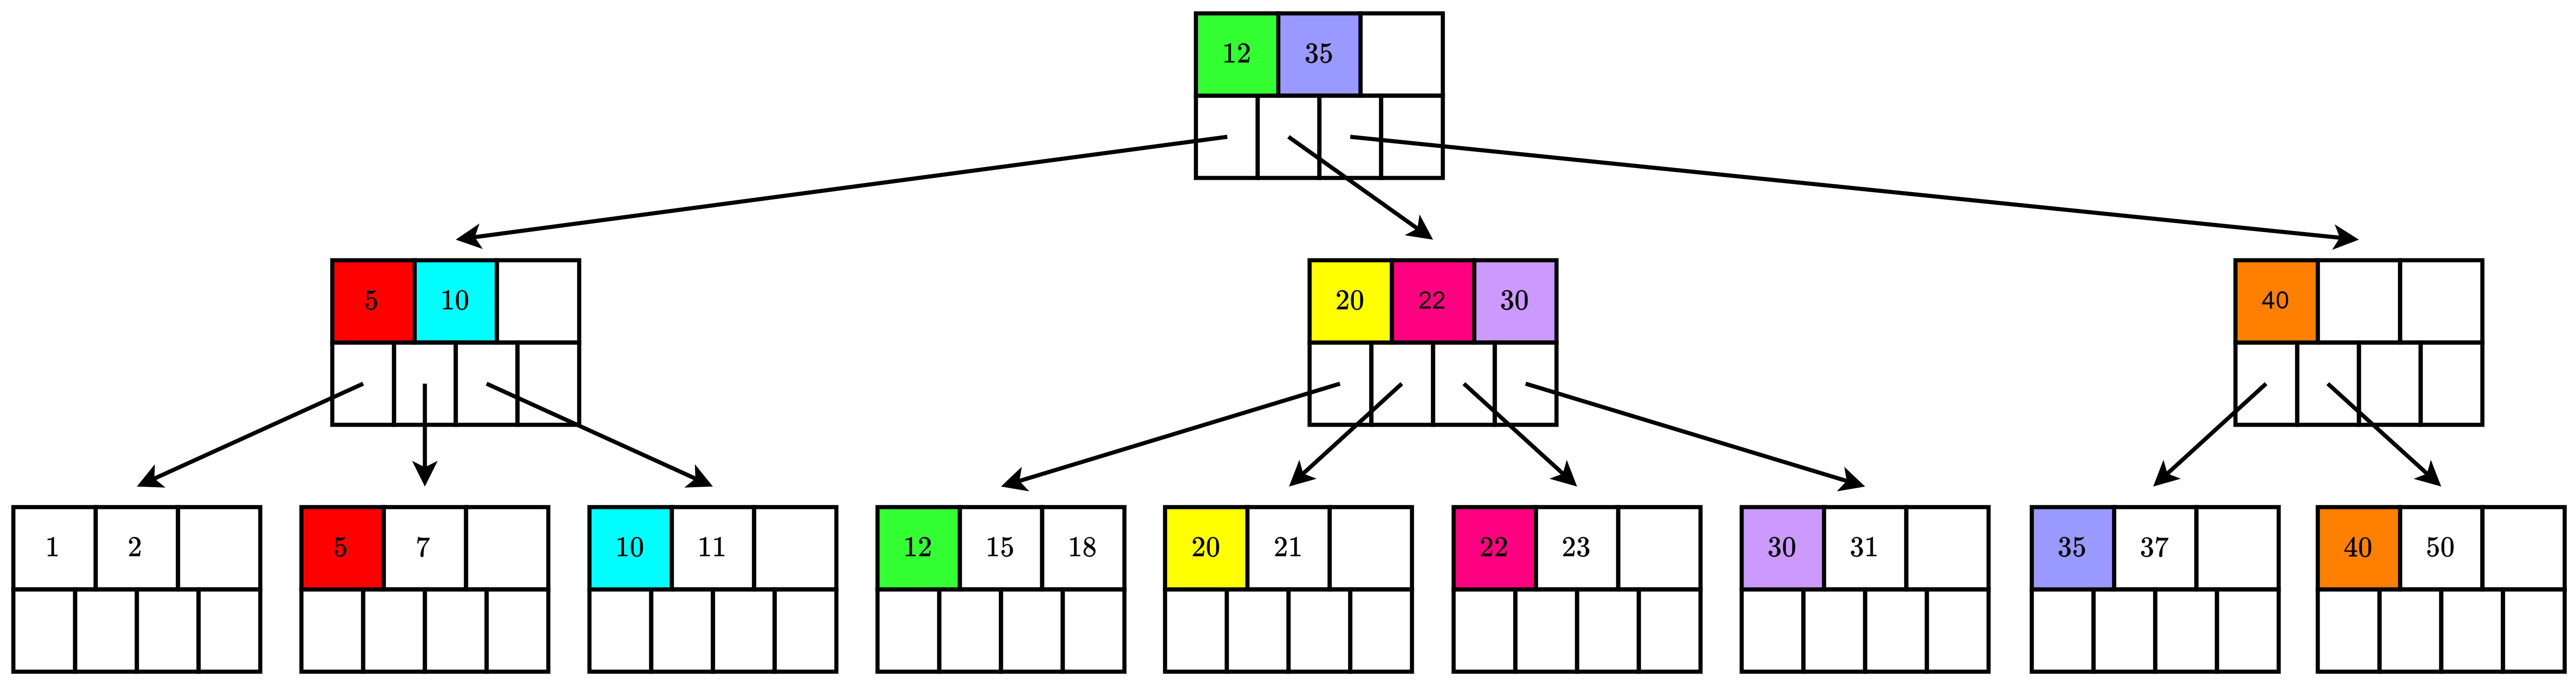
\includegraphics[width=0.8\textwidth]{diagram/P3-1-19-2.png}
                \end{figure}

                \item Ingresa 45:
                \begin{figure}[H]
                    \centering
                    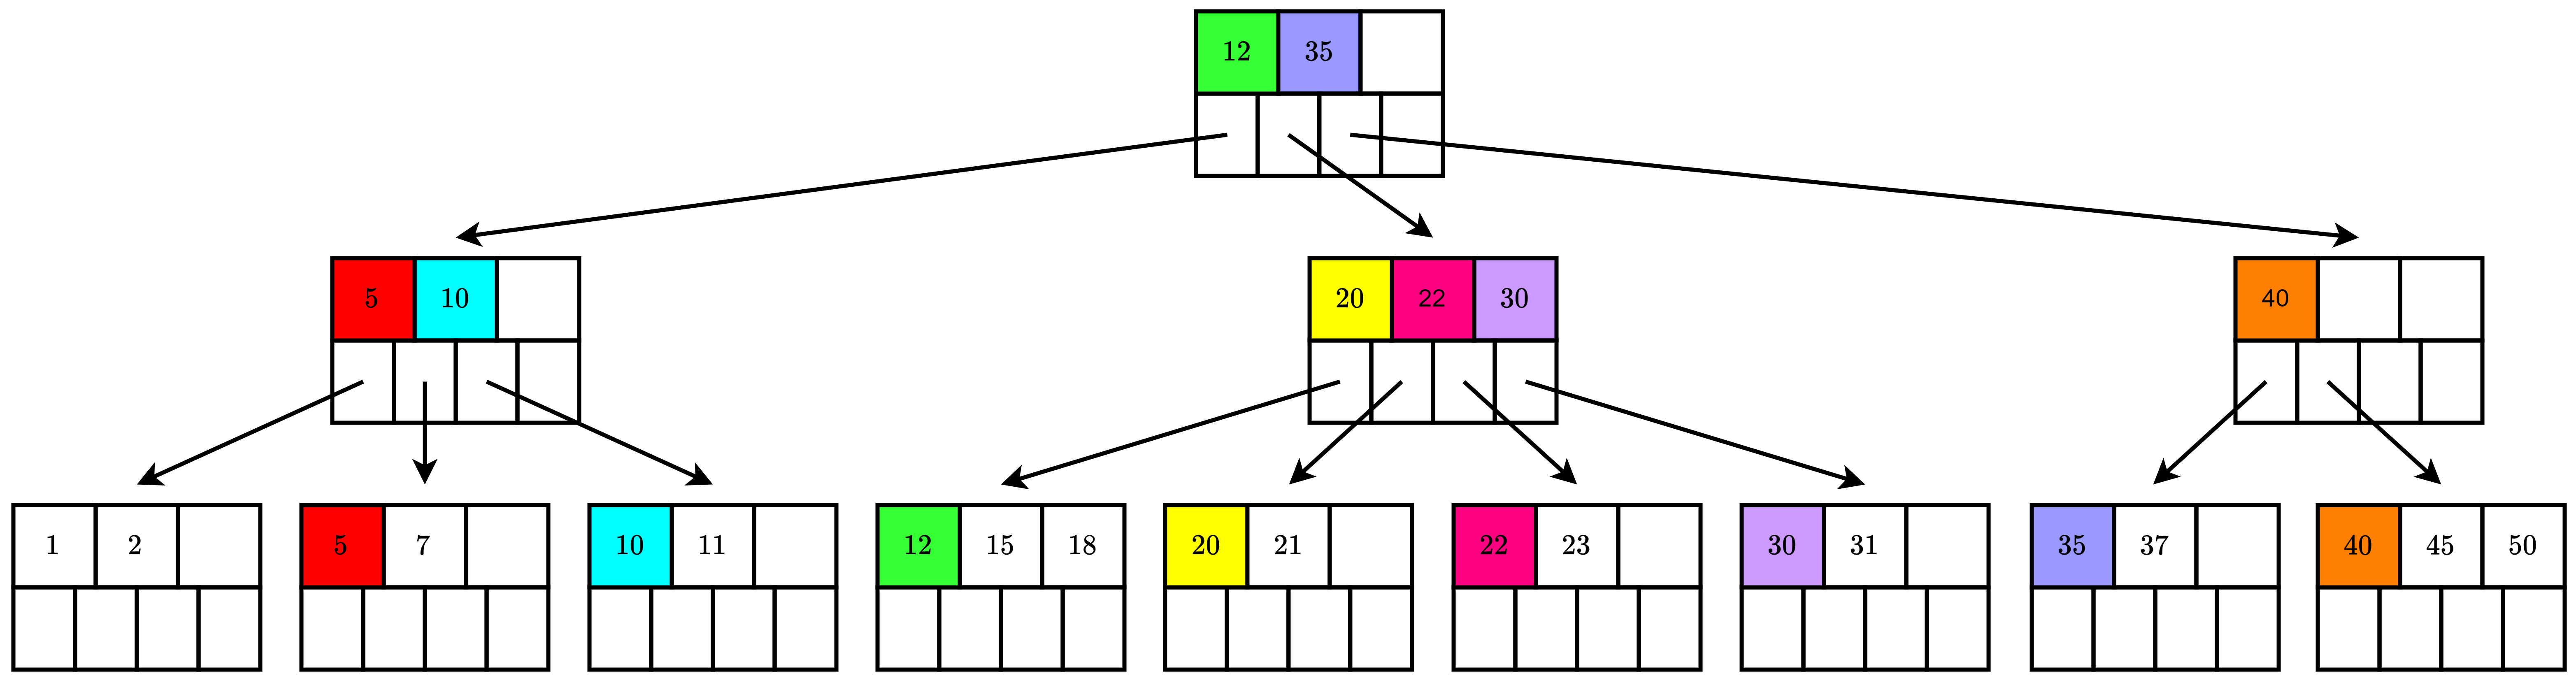
\includegraphics[width=0.8\textwidth]{diagram/P3-1-20.png}
                \end{figure}

                \item Ingresa 56:
                \begin{figure}[H]
                    \centering
                    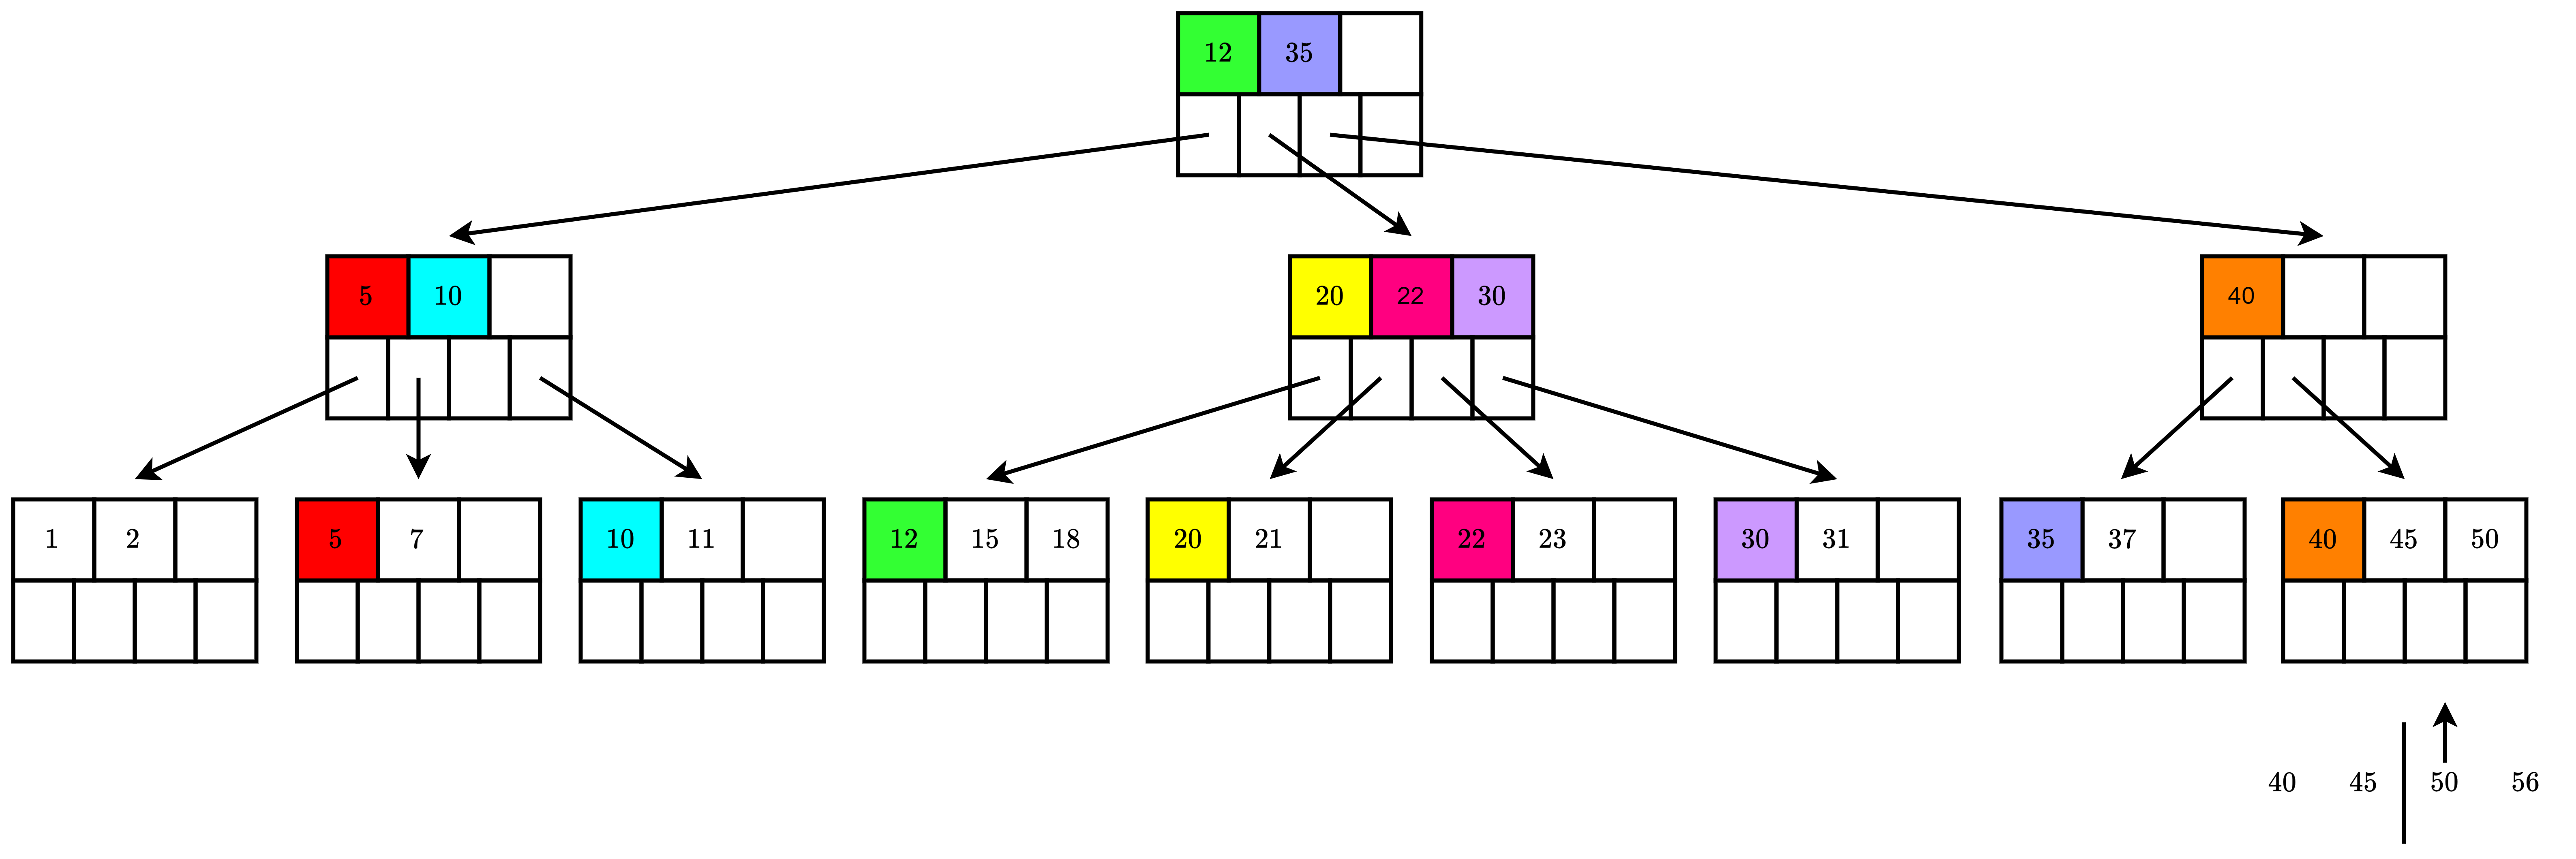
\includegraphics[width=0.8\textwidth]{diagram/P3-1-21-1.png}
                    \rule{\textwidth}{1pt}
                    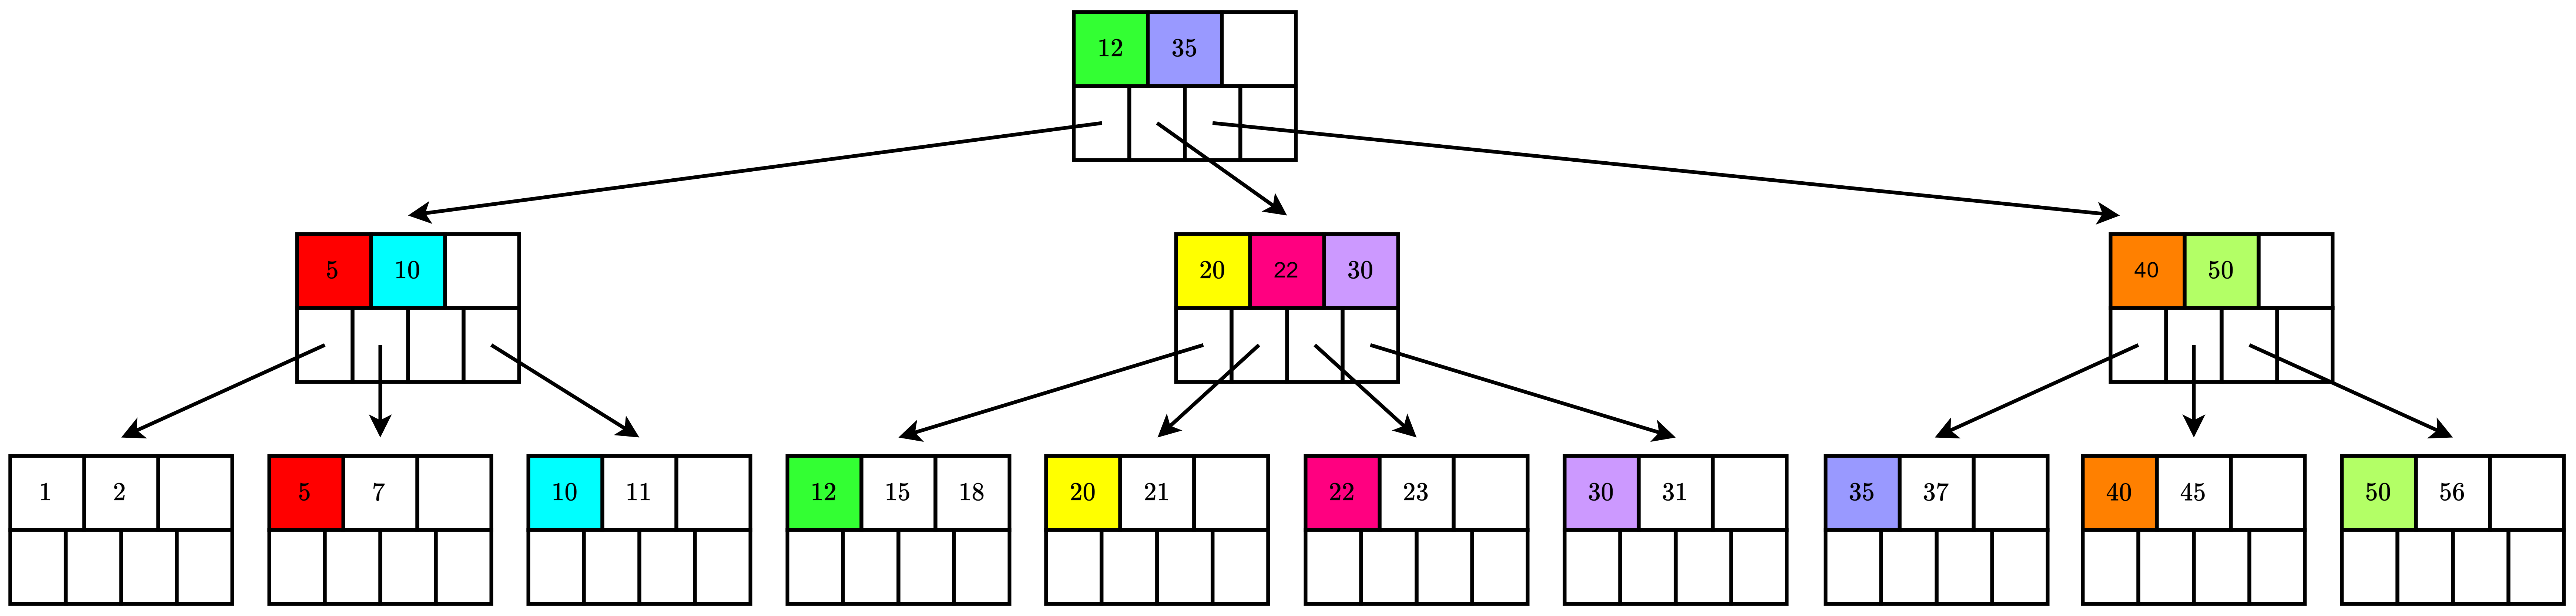
\includegraphics[width=0.9\textwidth]{diagram/P3-1-21-2.png}
                \end{figure}

                \item Ingresa 57:
                \begin{figure}[H]
                    \centering
                    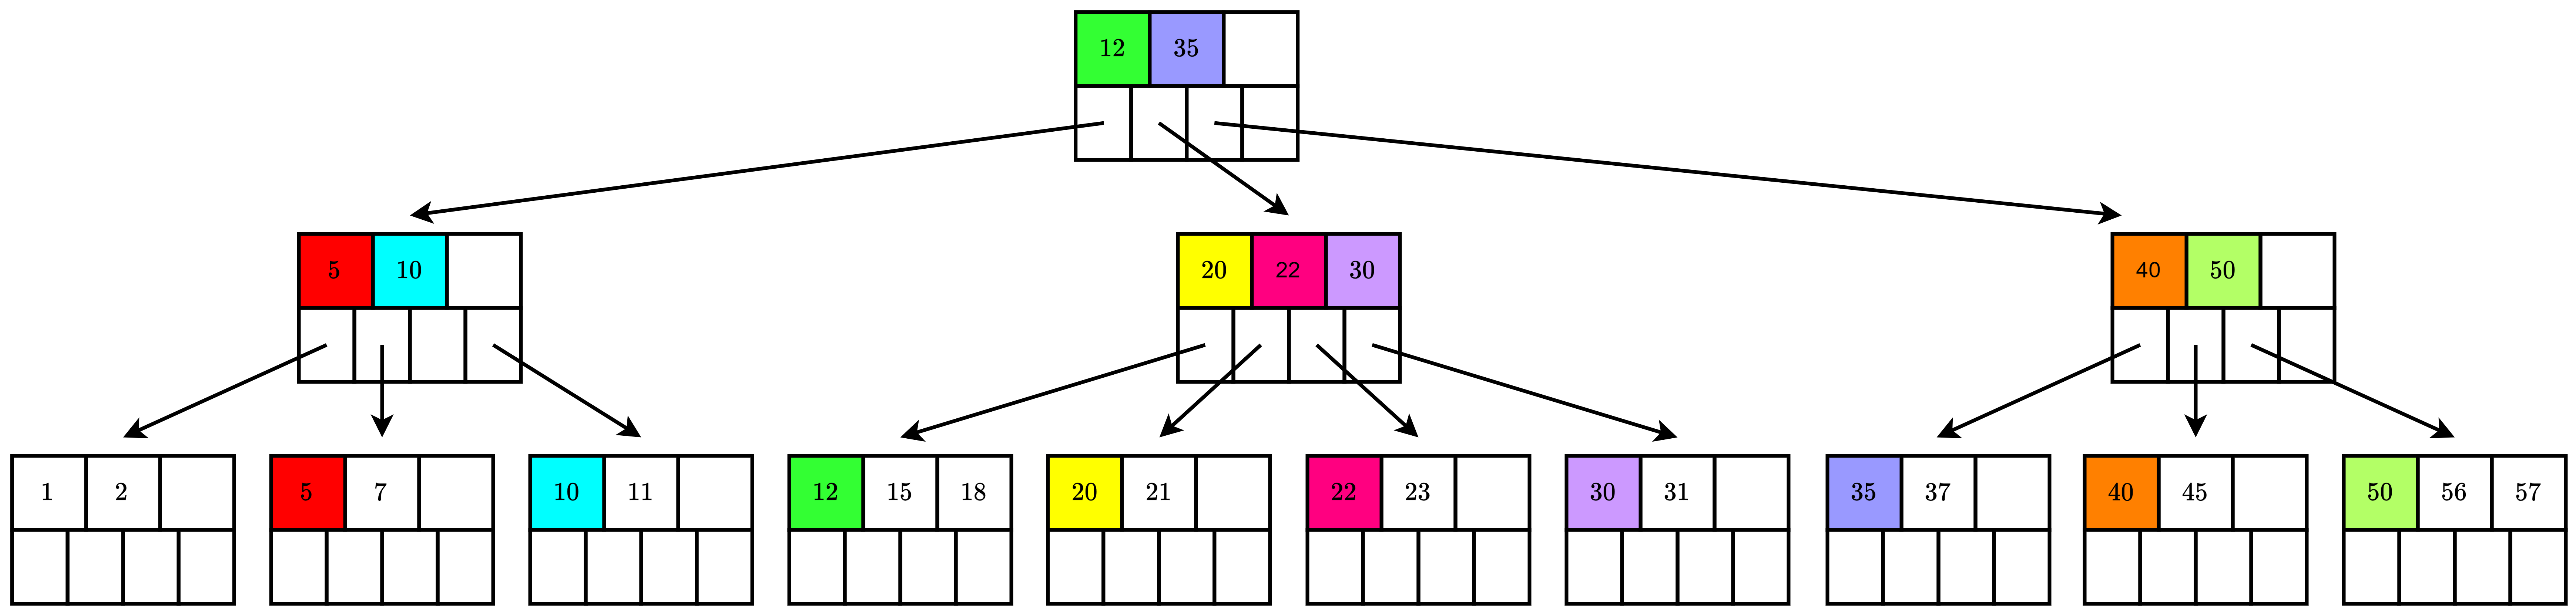
\includegraphics[width=\textwidth]{diagram/P3-1-22.png}
                \end{figure}

                \item Ingresa 60:
                \begin{figure}[H]
                    \centering
                    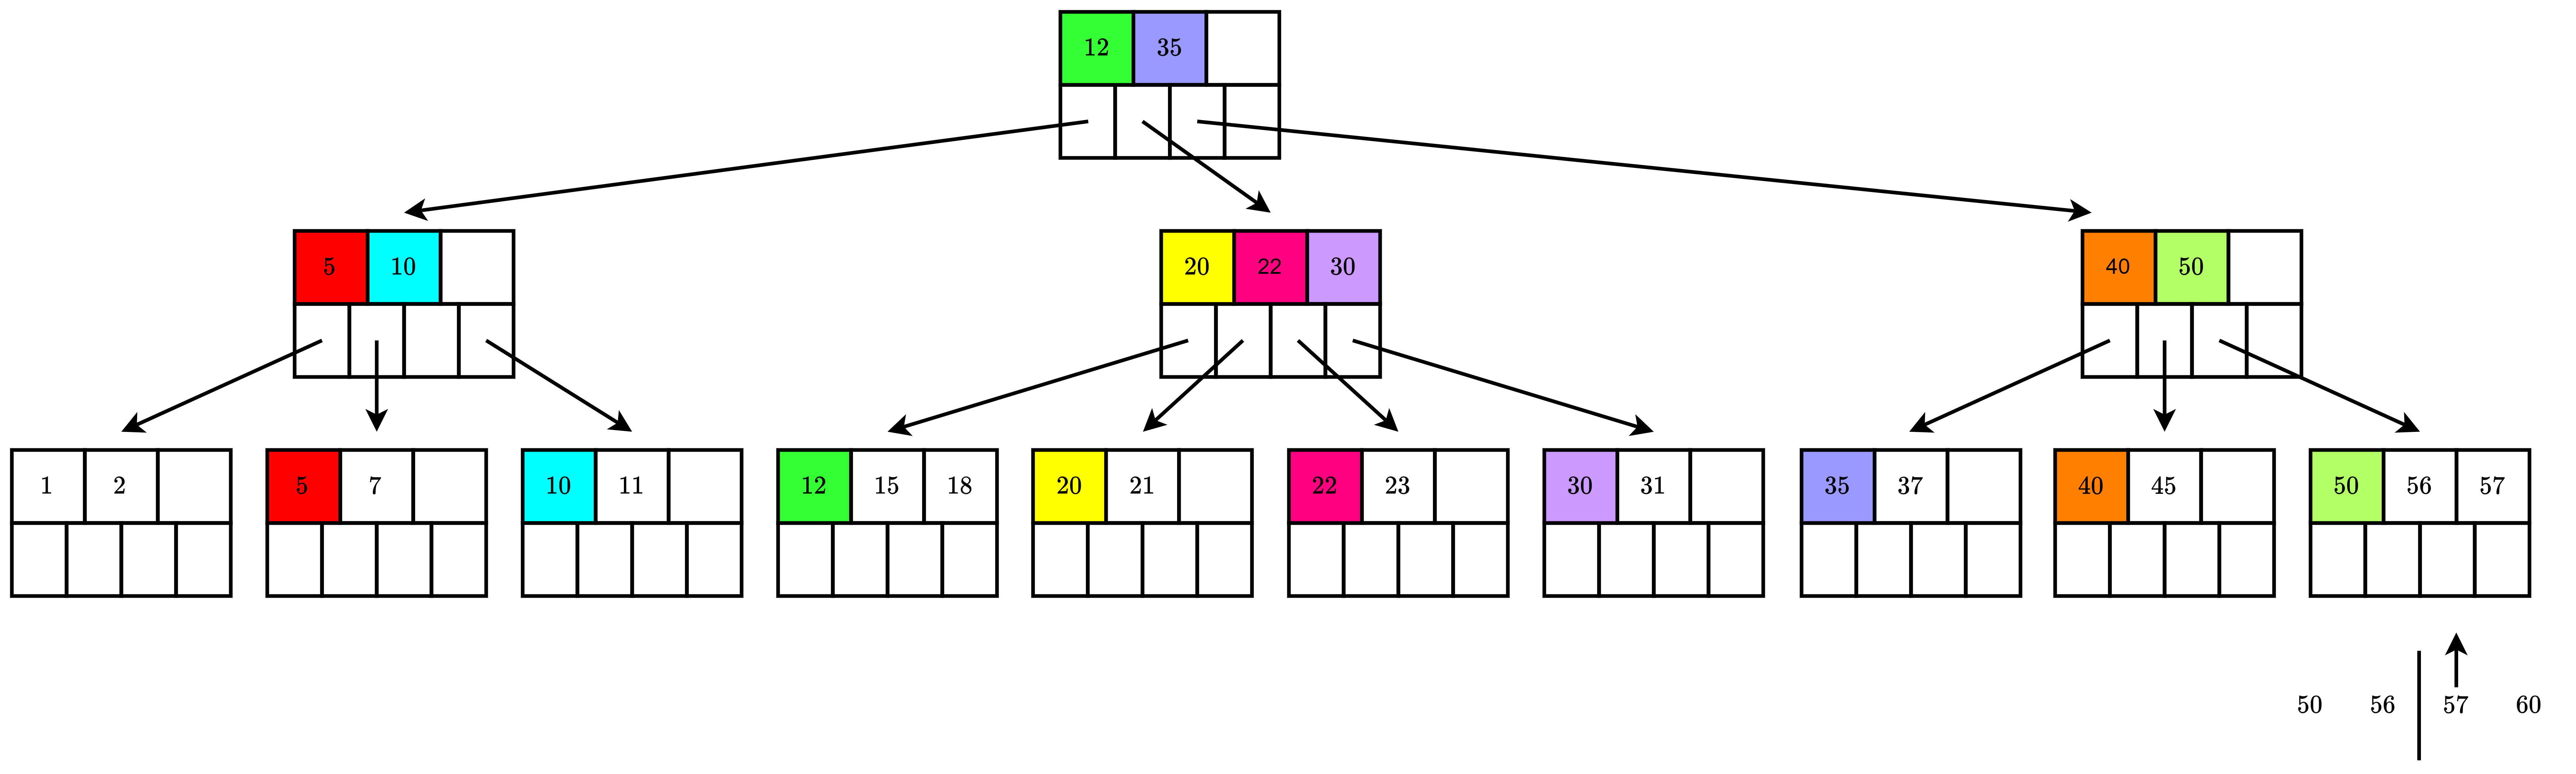
\includegraphics[width=\textwidth]{diagram/P3-1-23-1.png}
                    \rule{\textwidth}{1pt}
                    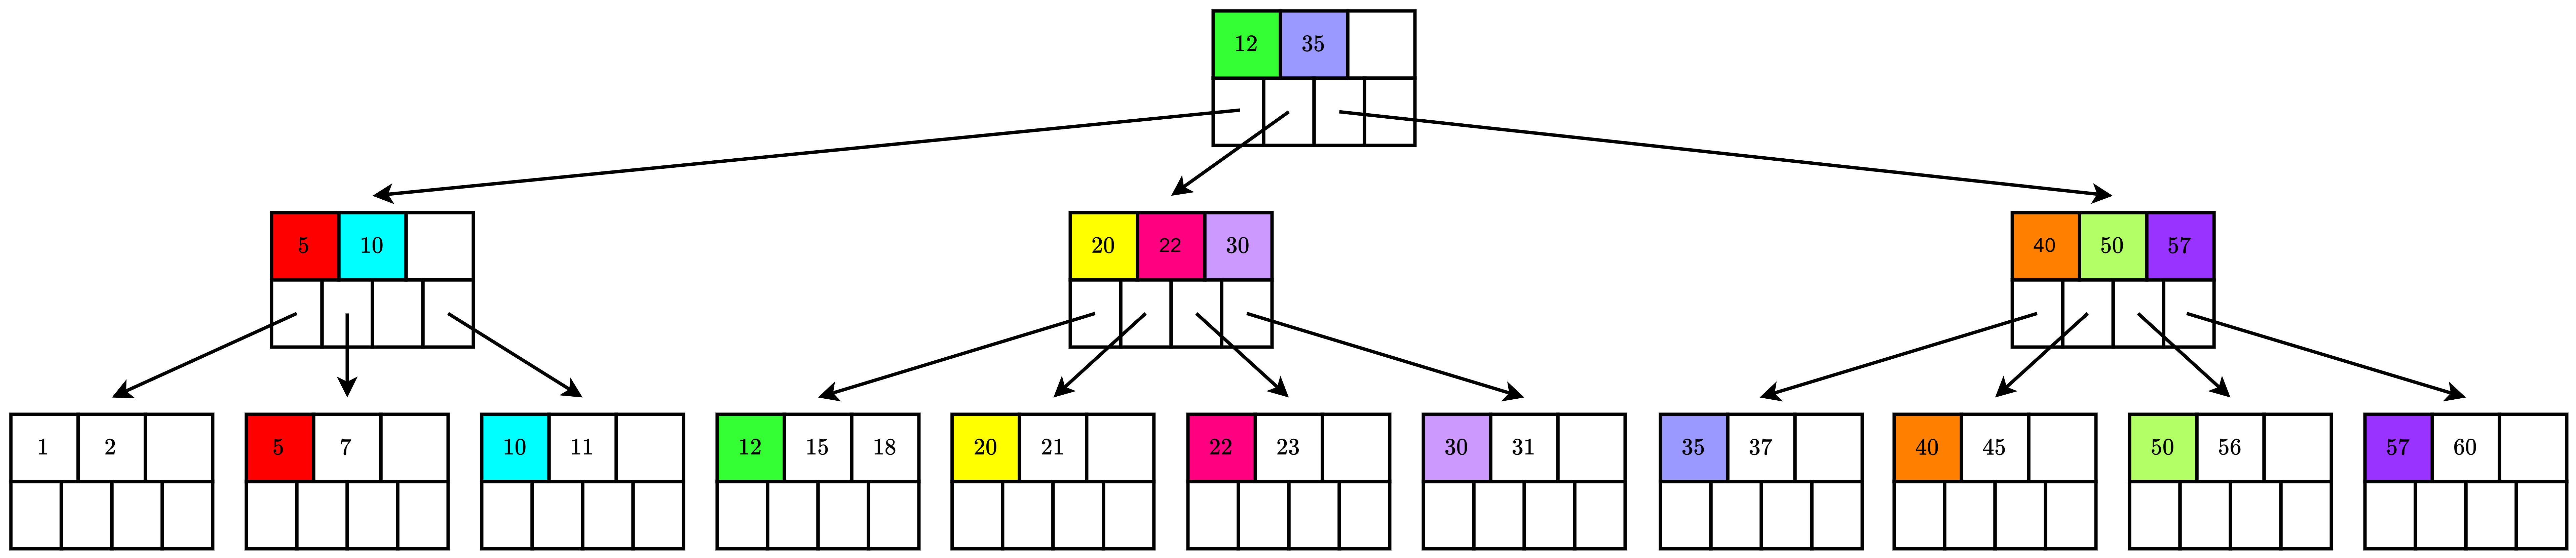
\includegraphics[width=\textwidth]{diagram/P3-1-23-2.png}
                \end{figure}
                
            \end{enumerate}
        \end{enumerate}

        \newpage
        \item $C = \{2,3,5,7,11,13,17,19,23,29,31,37,41,43,47\}$.
        \begin{figure}[H]
            \centering
            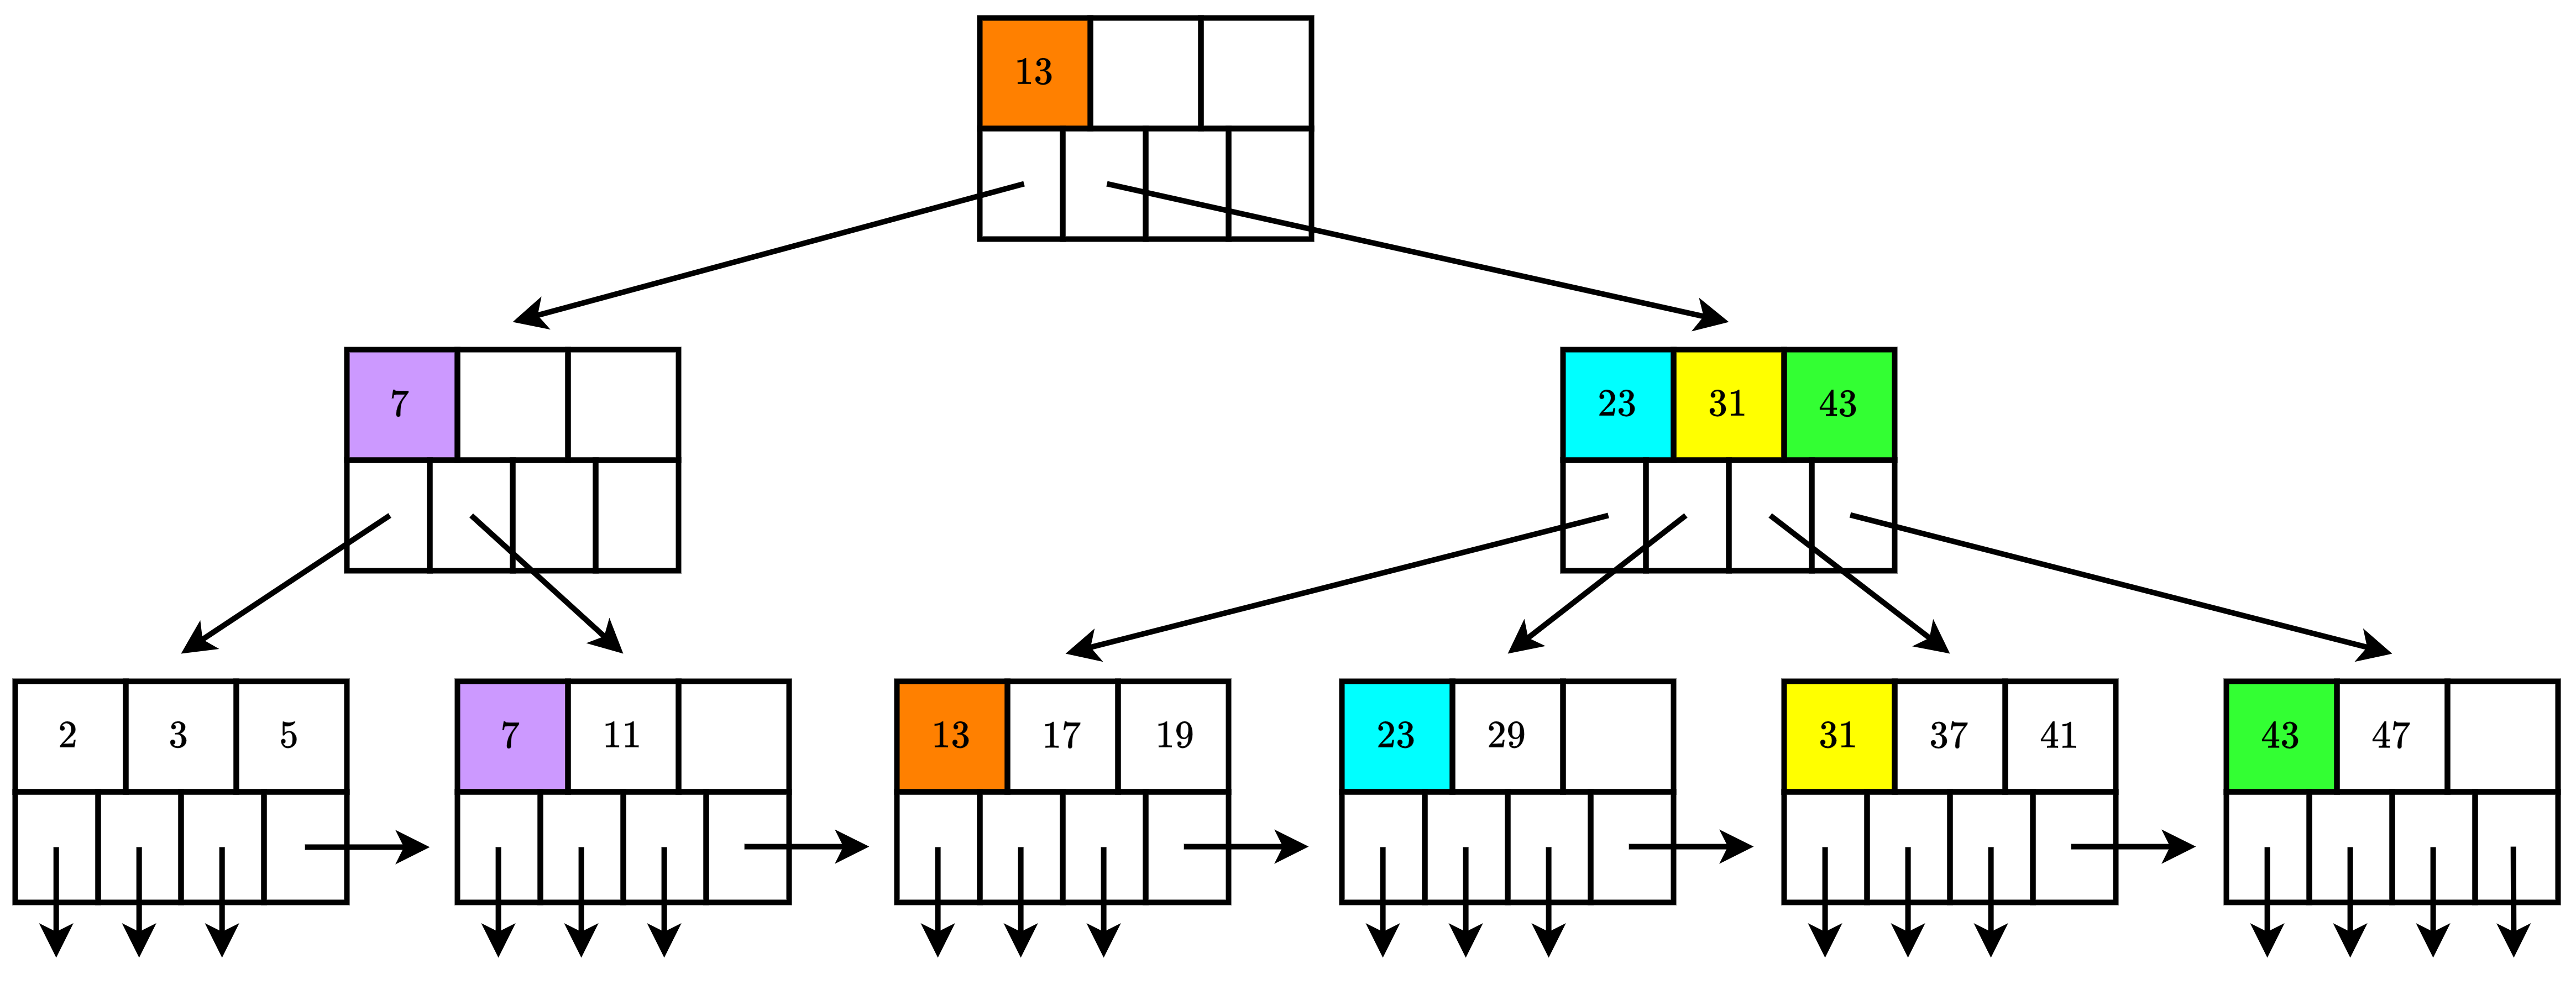
\includegraphics[width=\textwidth]{diagram/P3-2.png}
        \end{figure}
        \begin{enumerate}
            \renewcommand{\labelenumi}{\alph{enumi})}
            \item Elimine la clave 23 del árbol B.
            \begin{figure}[H]
                \centering
                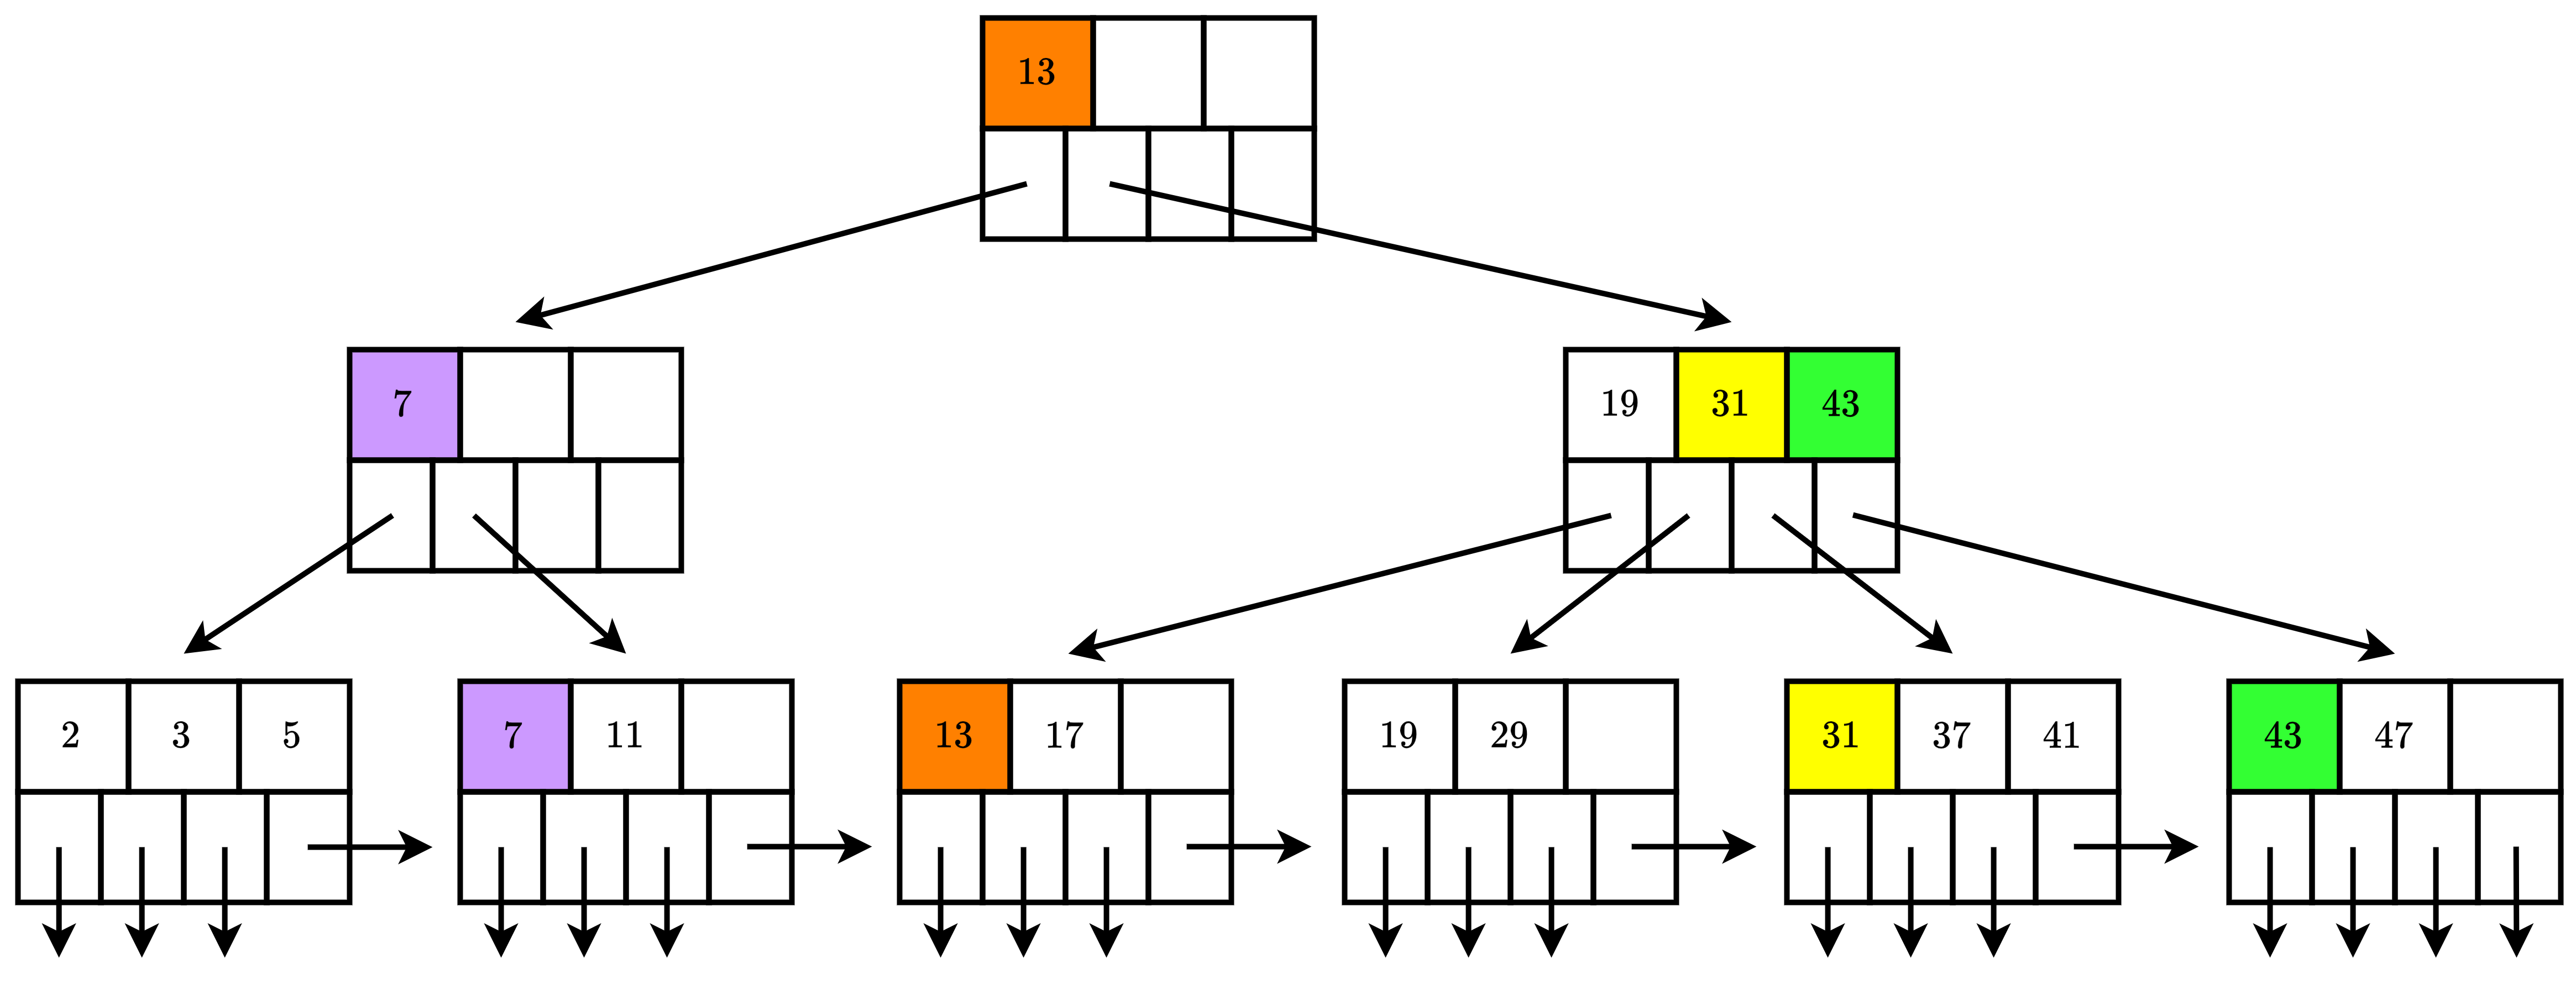
\includegraphics[width=\textwidth]{diagram/P3-2-a.png}
            \end{figure}

            \item Luego elimine la clave 29 del árbol B.
            \begin{figure}[H]
                \centering
                \includegraphics[width=\textwidth]{diagram/P3-2-b.png}
            \end{figure}

            \newpage
            \item Muestre y explique que pasos realizó para eliminar ambos valores.
            
            \textcolor{red}{Cuando se elimina la clave 23, al ser importante para el árbol, se juntan los datos $13,17,19$ y $29$, luego se divide esta lista en 2 y sube como valor principal el $19$.
                \begin{figure}[H]
                    \centering
                    \includegraphics[width=\textwidth]{diagram/P3-2-c.png}
                \end{figure}
                Para eliminar la clave 29, es mas sencillo pues no es un valor importante para el árbol, por lo que se elimina directamente.
                \newline
                \textbf{OBS: No se realmente como explicarlo de una forma formal.}
            }
        \end{enumerate}
    \end{enumerate}
\end{itemize}   
\end{document}